%%%%%%%%%%%%%%%%%%%%%%% file template.tex %%%%%%%%%%%%%%%%%%%%%%%%%
%
% This is a general template file for the LaTeX package SVJour3
% for Springer journals.          Springer Heidelberg 2010/09/16 
%
% Copy it to a new filxe with a new name and use it as the basis
% for your article. Delete % signs as needed. 
%
%%%%%%%%%%%%%%%%%%%%%%%%%%%%%%%%%%%%%%%%%%%%%%%%%%%%%%%%%%%%%%%%%%
%
\RequirePackage{fix-cm} 
%
%\documentclass[referee,natbib]{svjour3}
                     % onecolumn (standard format)
\documentclass[natbib]{svjour3}

\smartqed % flush right qed marks, e.g. at end of proof
%
\usepackage{graphicx}
\usepackage{booktabs}
\usepackage{textcomp}
\usepackage{lineno}
\usepackage{multirow}
\usepackage{xcolor}
\usepackage{enumitem}
\usepackage[version=3]{mhchem}
\usepackage{array}
\usepackage{subfig}
\usepackage{subfloat}
\usepackage{float}
\usepackage[section]{placeins}
\usepackage{natbib}
\usepackage{latexsym}
\usepackage{authblk}
\usepackage{upquote,textcomp}

\newcommand\Mark[1]{\textsuperscript#1}

\definecolor{revision}{rgb}{0.0,0.0,1.0}
%\definecolor{revision}{rgb}{0.0,0.0,0.0} % use this to remove color
\newcommand{\revision}[1]{{\color{revision} {#1}}} % track changes: add new text

% \usepackage{mathptmx}% use Times fonts if available on your TeX system
% * <lara.panossian@jpl.nasa.gov> 2018-04-19T16:29:28.216Z:
%
% ^.
%
% insert here the call for the packages your document requires
%\usepackage{latexsym}
% etc.
%
% please place your own definitions here and don't use \def but
% * <lara.panossian@jpl.nasa.gov> 2018-04-16T12:49:56.811Z:
%
% ^.
% \newcommand{}{}
%
% Insert the name of "your journal" with
 \journalname{Space Science Reviews}
%

\begin{document}

\title{Pre-Mission InSights on the Interior of Mars}
\titlerunning{Pre-Mission InSights on the Interior of Mars}        % if too long for running head
\authorrunning{Smrekar et al.} % if too long for running head

\author{Suzanne E.	Smrekar$^1$
\and	Philippe 	Lognonn\'e$^2$
\and	Tilman	Spohn$^3$
\and	W. Bruce Banerdt$^1$
\and	Doris	Breuer$^3$
\and	Ulrich	Christensen$^4$
\and	V\'eronique	Dehant$^5$
\and	M\'lanie	Drilleau$^2$
\and	William	Folkner$^1$
\and	Nobuaki	Fuji$^2$
\and	Raphael	F. Garcia$^6$
\and	Domenico	Giardini$^7$
\and	Matthew	Golombek$^1$
\and	Matthias	Grott$^3$
\and	Tamara	Gudkova$^8$
\and	Catherine	Johnson$^{9,10}$
\and	Amir	Khan$^7$
\and	Benoit	Langlais$^{11}$
\and	Anna	Mittelholz$^9$
\and	Antoine	Mocquet$^{11}$
\and	Robert	Myhill$^{12}$
\and	Mark	Panning$^1$
\and	Cl\'ement	Perrin$^2$
\and	Tom	Pike$^13$
\and	Ana-Catalina Plesa$^3$
\and	Attilio	Rivoldini$^5$
\and	Henri	Samuel$^2$
\and	Tim	Van Hoolst$^5$
\and	Olivier	Verhoeven$^{11}$
\and	Renee	Weber$^{14}$
\and	Mark	Wieczorek$^{15}$}


%% AUTHORS' AFFILIATION
\institute{Suzanne E. 	Smrekar\\
\email{ssmrekar@jpl.nasa.gov}\\
$^1$ Jet Propulsion Laboratory, California Institute of Technology, 4800 Oak Grove Drive, Pasadena, CA 91109,
United States \\
$^2$ Univ Paris Diderot-Sorbonne Paris Cit\'e, Institut de Physique du Globe de Paris, 35 rue H\'{e}l\`{e}ne Brion - Case 7071,
Lamarck A - 75205 Paris Cedex 13, France \\
$^{3}$ German Aerospace Center (DLR), Rutherfordstrasse 2, 12489 Berlin, Germany \\
$^4$ Max Planck Institute for Solar System Research, G\"ottingen, Germany\\
$^{5}$ Royal Observatory Belgium, Av Circulaire 3-Ringlaan 3, 1180 Brussels, Belgium \\
$^6$ Institut Superieur  de l'Aeronautique et de l'Espace, Toulouse, France \\
$^{7}$ Institut f\"{u}r Geophysik, ETH Z\"{u}rich, 8092 Z\"{u}rich, Switzerland \\
$^{8}$ Schmidt Institute of Physics of the Earth RAS, Moscow, Russia \\
$^{9}$ University of British Columbia, Canada \\
$^{10}$ Planetary Science Institute, Pasadena, CA, USA\\
$^{11}$ Laboratoire de Plan\'{e}tologie et G\'{e}odynamique, UMR-CNRS 6112, Universit\'{e} de Nantes, Facult\'{e} des Sciences et
Techniques,  Nantes, France \\
$^{12}$ School of Earth Sciences, University of Bristol,  Bristol, United Kingdom \\
$^{13}$ Department of Electrical and Electronic Engineering, Imperial College, London, United Kingdom \\
$^{14}$ NASA Marshall Space Flight Center, 320 Sparkman Drive, Huntsville, AL 35805, United States \\
$^{15}$ Observatoire de la C\^ote d'Azur, Nice, France\\
} 

\date{Received: date / Accepted: date}
% The correct dates will be entered by the editor

\maketitle

  
\begin{abstract}
The Interior exploration using Seismic Investigations, Geodesy, and Heat Transport (InSight) Mission will focus on Mars' interior structure and evolution.  The basic structure of crust, mantle, and core form soon after accretion.  Understanding the early differentiation process on Mars and how it relates to bulk composition is key to improving our understanding of this process on rocky bodies in our solar system, as well as in other solar systems.  Current knowledge of differentiation derives largely from the layers observed via seismology on the Moon.  However, the Moon's much smaller diameter make it a poor analog with respect to interior pressure and phase changes.  In this paper we review the current knowledge of the thickness of the crust, the diameter and state of the core, seismic attenuation, heat flow, and interior composition. InSight will conduct the first seismic and heat flow measurements of Mars, as well as more precise geodesy.  These data reduce uncertainty in crustal thickness, core size and state, heat flow, seismic activity and meteorite impact rates by a factor of 3-10X relative to previous estimates.  Based on modeling of seismic wave propagation, we can further constrain interior temperature, composition, and the location of phase changes.  By combining heat flow and a well constrained value of crustal thickness, we can estimate the distribution of heat producing elements between the crust and mantle. All of these quantities are key inputs to models of interior convection and thermal evolution that predict the processes that control subsurface temperature, rates of volcanism, plume distribution and stability, and convective state.  Collectively these factors offer strong controls on the overall evolution of the geology and habitability of Mars.
\end{abstract}

{\keywords{Mars \and InSight \and Interior \and seismology \and heat flow \and geodesy \and crust \and mantle \and core}}


\newpage
\section{Introduction \label{sec:introduction}}The first step in planet formation is accretion of planetesimals.  If accretion results in sufficient mass and energy to melt the initial body, all planetary bodies will differentiate into at least three compositional layers:  the dense core at the center, an intermediate density mantle, and a buoyant crust at the surface \citep{Elkins-Tanton2011a}.  The precise thickness of these layers and details such as the state (molten and/or solid) of the core, the temperature of mantle, and any layering in the crust, contain important information about the processes that shape the overall evolution of a planet \citep{Mocquet2011}.  Processes such as magma ocean formation and overturn, convective style and lithospheric mobility all shape interior structure and thermal evolution.  Global overturn models also make predictions about final crustal thickness.  The key variables in models of crust formed via accumulation of melt products above a convecting mantle predict a large range of crustal thickness.  The modeled production of crust via pressure release melting in a convecting mantle is strong function of temperature and volatile content.   If present on early Mars, plate tectonics would have cooled Mars more rapidly than stagnant lid convection. The thickness and state of the mantle and core affect the geometry and heat loss rate of convection, and thus the history of volcanism and volatile outgassing.

The intermediate size of Mars between Earth and the Moon, the only two bodies for which seismic and heat flow data have been acquired to date, places it in the sweet spot for understanding early planetary formation. The Moon's diameter limits the phase transitions in the interior to those occurring at relative shallow depths on Earth \citep{Khan_etal13, Kuskov2014}, thus limiting applicability to larger bodies. Mars is large enough to be in the same pressure regime as Earth’s upper mantle, small enough to be geologically arrested enough to preserve its original crust.  Mars’ relatively small volume also means that it contains insufficient heat producing elements to maintain vigorous present day geologic activity, thus preserving much of its original crust. Additionally, there is a wealth of data for Mars, including from both missions and meteorites, that provide strong constraints on its original composition and geologic evolution. 
\begin{figure}[h!]
\begin{center}
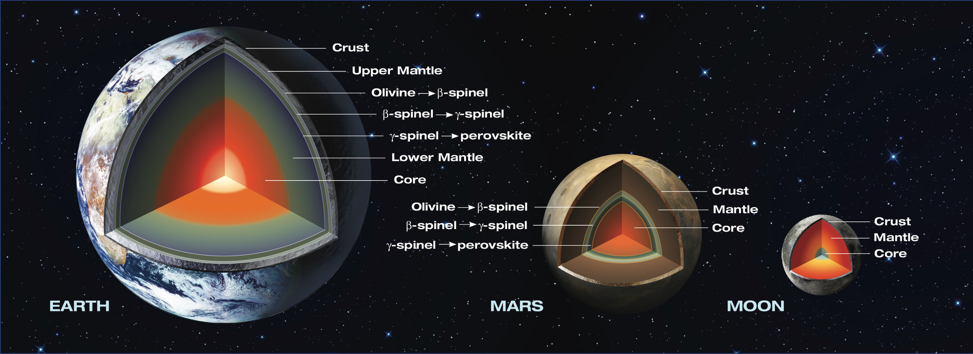
\includegraphics[width=0.95\textwidth]
{figures/Fig1_1.png}
\caption{Interior structure of Earth, Mars and the Moon, with known phase transitions for Earth and possible phase transition locations for Mars.}
\label{fig:Fig1_1.png} 
\end{center}
\end{figure}

The InSight mission will provide the first seismic and heat flow data for Mars, enabling unprecedented constraints on interior structure and evolution.  InSight launches in May of 2018, and arrives at Mars on November 26, 2018, landing on Elysium Planitia \citep{Golombek2017}.  The three primary instruments are the Seismic Experiment for Interior Structure (SEIS), the Heat Flow and Physical Properties Package (HP$^3$), and the Rotation and Interior Structure Experiment (RISE).   SEIS consists of a set of 3 very broad band seismometers coupled with 3 short period seismometers \citep{Lognonne2018}. Techniques for determining interior structure with a single station are described in \citet{PANNING2015,BOSE2017}. HP$^3$ is a self-hammering mole that deploys a tether with embedded temperature sensors to a depth of 3-5 m, taking thermal conductivity measurements as it descends \citep{Spohn2018}.  RISE \citep{Folkner2018} uses two low gain X-band antennas to precisely track the lander location over a Martian year to determine the rotation of Mars, as well as its precession and nutation. RISE data will enable the first estimate of Mars’ nutation, thus providing tight constraints on core size, density and state (liquid versus solid).  The lander Instrument Deployment Arm \citep{Trebi-Ollennu2018} will deploy SEIS and HP$^3$ on the surface of Mars, with the aid of two cameras to image the deployment zone \citep{Maki2018}.  Additionally, a pressure sensor, wind sensors, and a magnetometer are used to decorrelate seismic events from atmospheric effects or lander magnetic field variations (Banfield et al., 2018). The HP$^3$ experiment includes a radiometer to determine surface temperature variations \citep{Spohn2018}. Finally, color images of the surface as well as experiments with the arm and scoop coupled with information from SEIS and HP will be used to better understand the geology and physical properties of the surface and shallow subsurface \citep{Golombek2018}


Using data from its three primary instruments, InSight will accomplish six science objectives \citep{Banerdt2013}:
\begin{itemize}
\item Determine the size, composition and physical state of the core
	\item Determine the thickness and structure of the crust
	\item Determine the composition and structure of the mantle
	\item Determine the thermal state of the interior
	\item Measure the rate and distribution of internal seismic activity
\item Measure the rate of impacts on the surface
\end{itemize}

In this paper, we will begin by summarizing the available constraints on the interior of Mars.  We then describe the theoretical framework for models of the interior structure and thermal evolution including equations of state, convection models, and their interdependence. Finally, we describe an approach to integrating the new constraints to be provided by InSight into a new framework for understanding early differentiation, core formation, dynamo history, mantle mineralogy and volatile content, thermal evolution including dynamo history, and crustal formation processes. 


\newpage
\section{Available Constraints on the Martian Interior \label{sec:constraints}}\subsection{Geologic history}

The geologic history of Mars provides key constraints on interior evolution. The cratering record shows that much of the crust formed very early in Martian history.  Both the hemispheric dichotomy between the southern highlands and northern lowlands and the huge Tharsis volcanic complex provide important constraints on interior structure and evolution. 

Impact crater density is used to divide the history of Mars into fours periods  (see \cite{Werner2011} 2011 for discussion and possible alternate dates): Pre-Noachian (\textgreater 4.1 Ga), Noachian (4.1-3.8 Ga), Hesperian (3.8-3.0 Ga), and Amazonian (\textless 3.0 Ga).  Much of the crust is Hesperian or older, making Mars an ideal location to study initial crustal formation.  The largest impact basins have locally excavated the crust.  The Hellas and Isidis basins are similar in size (see Figure \ref{fig:topo}), but have very different depths and gravity signatures due to subsequent filling of Isidis \citep{Searls2006}. The largest basin, Utopia, is located in the northern plains and is completely buried.  As discussed below, the entire northern hemisphere may have formed as a result of a very early impact, or via endogenic processes. High resolution topography revealed numerous impact basins buried under 1-2 km of fill in the northern plains, implying formation in the Pre-Noachian \citep{Nimmo2005, Frey2006}. Younger, Amazonian age features consist of polar cap ice deposits, volcanism, sediments, and impacts. The InSight landing site in Elysium Planitia, is located near some of the youngest volcanic and tectonic features on the planet \citep{Vaucher2009, Burr2002}, potentially providing seismic sources \citep{Roberts2012, Taylor2013}.
The most prominent topographic features are the dichotomy between the northern and southern hemispheres and the Tharsis volcanic rise. Each of these features are clearly visible in the topography of Mars (Figure \ref{fig:topo}), and relate directly to interior processes or crustal structure.

\begin{figure}[h!]
\begin{center}
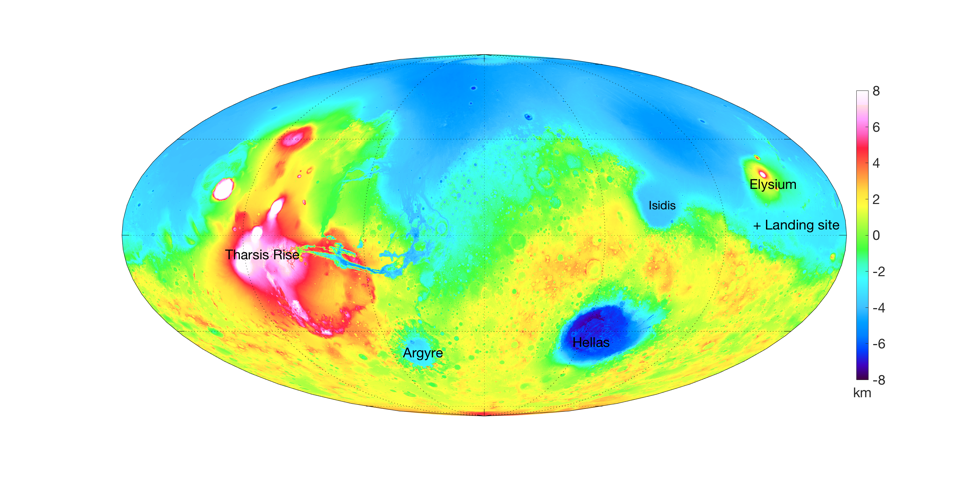
\includegraphics[width=0.85\textwidth]
{figures/Fig_2New.png}
\caption{Key topographic features on Mars include the hemispherical dichotomy, separating the northern lowlands from the southern highlands, the Tharsis volcanic complex, and major impact basins, as labeled.}
\label{fig:topo} 
\end{center}
\end{figure}

The southern highlands are on average 4-5 km higher than the northern lowlands (Figure \ref{fig:topo}), and have a much higher crater density due to infilling of the northern plains by volcanism and sediments. The origin of dichotomy has been attributed to both endogenic processes such as hemispherical scale (degree 1) mantle convection \citep{SCHUBERT1973,Wise1979a,Wise1979, Breuer1997, Breuer1998, Zhong2001} or very early plate tectonic \citep{Sleep1994}. Exogenic models include single \citep{Wilhelms1984} or multiple \citep{Frey1988} impact events. In some scenarios, a degree-1 plume formed under the southern hemisphere and caused massive melting that thickened the crust and produced higher elevation in the south via isostatic adjustment \citep{Zhong2001}.  Alternatively, a degree-1 plume may have thinned the crust in the northern lowlands \citep{Roberts2006}. Another proposed mechanism is the overturn of a buoyantly unstable mantle following magma ocean solidification \citep{Elkins-Tanton2008}. \citep{Andrews-Hanna2008} proposed that the northern plains were formed via a single impact that created an elliptical basin, as predicted by modeling\citep{Marinova2008}. They used both gravity and topography to remove the signature of Tharsis and Arabia Terra on the shape of the northern plains. 

These models have different implications for the composition and structure of the interior. A major question has been whether there is a difference in crustal composition between the north and the south that contributes to the difference in elevation.  A recent investigation of the northern lowlands basement composition, as revealed by impact crater excavations, finds a range of hydrated minerals beneath the surficial volcanic fill, similar in composition to those found in the southern highlands \citep{Pan2017}. Although the sampling depth is limited, this work strongly suggests that the difference in elevation reflects a difference in crustal thickness rather than composition.  Another puzzling question is why the northern lowlands exhibit very little crustal remnant magnetization relative to the southern highlands despite their similarity in age e.g. (e.g.,\cite{Langlais2004}).  One possible explanation is that the dynamo on Mars was asymmetric \cite{Stanley2008}.

Mars’ other major physiographic feature is the Tharsis rise, a massive volcanic complex.  It covers one quarter of the Martian surface and is the largest volcanic construct in the solar system (Figure \ref{fig:topo}).  The rise itself is ~10 km high, with three central volcanoes with heights of \textgreater 10 km each, in addition to Olympus Mons to the northwest and Alba Patera to the north (Figure \ref{fig:topo}).  This huge feature affects the global topography, gravity, and surface deformation  (see \citep{GolombekM.P.andPhillips2009PlanetaryTectonics}for a review). The age of the planetary scale deformation associated with Tharsis and the extensive volcanism indicate that the region has been active over most of the age of Mars. Although much of the topography is interpreted to have formed early in Martian history, modest volcanism persisted into the Amazonian.  For example, Arsia Mons may have been active as recently as 10-90 Ma \cite{Richardson2017}.  

The massive topography of Tharsis must be held up by some combination of compositional and/or thermal isostasy, flexure, and dynamic mantle support.  The exact proportion and origin of these mechanisms have implications for interior structure, mantle dynamics, and thermal evolution.  Models of loading of the lithosphere in response to Tharsis volcanism show that membrane stresses are capable of supporting the majority of the load \cite{Banerdt1982, Banerdt1992} and successfully predict more deformation features than isostatic models, even if coupled with a regional stress field \citep{Tanaka1991}.  Much of the lithospheric deformation dates to the Middle Noachian (\textgreater 3.8 Ga), and requires that the Tharsis load have the dimensions of the current topographic rise \cite{Phillips2001}.  Modeling of the present-day gravity and topography fields also predict the pattern of deformation, indicating that the stress fields have largely been unchanged since the Noachian \cite{Banerdt2000}. \citet{Bouley2016} proposed an alternative explanation, suggesting that the orientation of a key deformation feature, valley networks, can be explained by topographic gradients between the northern and southern hemispheres prior to Tharsis formation. In this scenario, major Tharsis construction begins in the Late Noachian.  One question for these loading models and interior structure is the degree of support due to low density mantle residuum \cite{Phillips1990}.

The Tharsis rise has been interpreted as forming over one or more mantle plumes.  The scale of plume, the formation of most of the volcanism early in Martian history, and the continuation of volcanic activity into recent Martian geologic history, have posed a challenge for convection simulations.  A series of convection models have shown that the presence of a phase transition near the core-mantle boundary supports the formation of a small number of plumes and areal concentration of plumes \citep{Harder1998,Harder2000,Harder1996,Breuer1998}. The size of the core is the dominant factor in determining whether or not phase transitions near the core-mantle boundary are present, and thus the applicability of such plume models. Another key challenge is for the convection pattern to localize rapidly enough to be consistent with timing constraints on the formation of Tharsis.  A key question is source of relatively recent volcanism given the very thick lithosphere under Tharsis. Modeling suggests that if present, a plume or other buoyant region at depth contributes only modestly to support of the topography \citep{Lowry2003,Zhong2003, Roberts2004, Redmond2004} Redmond and King, 2004).  Alternative ideas for the formation of Tharsis include warming of the mantle \cite{Solomon1982a}.  Warming might occur under a thick, insulating southern hemisphere crustal layer \cite{Wenzel2004}. 

\subsection{Composition}
Our current knowledge of the bulk chemical and mineralogical composition of Mars is based on the analysis of the Martian meteorites, remote sensing and in-situ analysis of the Martian surface as well as on geophysical properties of the planet.   

\subsubsection{Meteorites, remote sensing and in-situ analysis}
Martian meteorites partially referred to as SNC meteorites (shergottites, nakhlites, and chassignites) are igneous rocks of varying mafic to ultramafic igneous lithologies. The meteorites exhibit both intrusive and extrusive textures including: basalt and lherzolite (shergottites), orthopyroxenite (ALH 84001), clinopyroxenite (nakhlites), and dunite (Chassigny). Except for ALH 84001, a 4.5-Ga sample of the Noachian crust, all SNCs were extracted from Amazonian volcanic terrains. The most representative samples are the shergottites that show crystallization ages between 170 and 600 Ma (e.g., McSween and McLennan, 2014).  For characterizing the chemistry and mineralogy of igneous materials at the surface of Mars, remote sensing data are also available. Mineralogical information is generally obtained using the visible and infrared range of the electromagnetic spectrum \citep{Bandfield2000, Poulet2009}, whereas abundances of chemical elements are principally derived from gamma-rays \citep{Boynton2007} and neutron spectroscopy (Feldman et al. 2011). In general, the spectral analysis of the Martian surface does not provide a good match to the spectral signature of the SNC meteorites \cite{HAMILTON2003, Lang2009} and Martian meteorite-like lithologies represent only a minor portion of the dust-free surface. However, the distinctive mineralogical characteristics of SNCs (ferroan olivine and pyroxenes, sodic plagioclase) are commonly indicated by remote-sensing data. Igneous rocks have also been analyzed in-situ in both Gusev Crater (e.g.,\cite{Squyres2004}). These rocks also range from basaltic to cumulate rocks (e.g.,Dreibus et al., 2007; McSween et al., 2006; Ming et al., 2008; Squyres et al., 2006) but are much older (\textasciitilde 3.65 Ga) than shergottites \citep{Arvidson, Greeley2005} and have significantly different chemistry than basaltic shergottites (Filiberto et al., 2006; \citep{McSween2009}; Taylor et al., 2006). These findings challenge the use of the SNCs in defining diagnostic geochemical characteristics and in constraining compositional models for Mars. We also note that extensive sedimentary deposits composed of phyllosilicates and sulfates have been observed from orbit and by rovers in Gale crater and Meridiani Planum, but spectral data from orbit (Ehlmann et al. 2011; Ehlmann and Edwards. 2014) and chemical and mineralogical data from the surface \cite{DavisA.M.McSweenH.Y.Jr.&McLennan2005} Grotzinger et al. 2014) show that most are basaltic in composition or have been altered from an initial basaltic composition, indicating that the martian crust is basaltic in composition.

\subsubsection{Bulk composition}
\setcounter{tocdepth}{4} \setcounter{secnumdepth}{4}
\paragraph{Geochemical perspective}

Assuming that the SNC meteorites are representative of the Martian crust, models based on geochemical arguments \cite{Dreibus1984}\cite{Dreibus1984AccretionPlanets.,Dreibus&Wanke1985, Wanke1994, Lodders1997, Morgan1979, Sanloup1999}. \cite{Mohapatra&Murty2003} have been developed to estimate the composition of the bulk silicate portion of Mars (see Taylor, 2013, for a recent review). To derive the chemical composition of Mars from the chemical compositions of the Martian meteorites, two general approaches have been applied. The first approach uses the elemental correlations in the Martian meteorites, assuming that refractory elements are present in chondritic abundances \cite{Dreibus1984, Dreibus1984AccretionPlanets.,Dreibus&Wanke1985, Wanke1994, Halliday2001, Longhi1992, Taylor2013} whereas the second approach uses oxygen isotope systematics of the SNC meteorites and match them via mass balance equations to mixtures of different chondritic material \citep{Lodders1997,Sanloup1999, Burbine2004}. Table \ref{compositiontable} shows a compilation of 5 different models of the bulk composition of Mars. These compositions represent the primitive mantle of Mars, i.e., unaffected by magmatic processes such as magma ocean fractional crystallization and crust formation. 

\begin{table}[h!]
\centering
\label{comptable}
\begin{tabular}{lllllll}
                                                & MA    & DW    & LF    & SA    & TA   &  \\
                                                &       &       &       &       &      &  \\
Bulk crust \& mantle composition(wt.\%) 
in major oxides &       &       &       &       &      &  \\
\ce{SiO2}                                            & 41.59 & 44.4 & 45.39 & 47.79 & 43.7 &  \\
\ce{Al2O3}                                          & 6.39  & 3.02  & 2.89  & 2.52  & 3.04 &  \\
MgO                                             & 29.77 & 30.2 & 29.71 & 27.46 & 30.5 &  \\
CaO                                             & 5.16  & 2.45  & 2.36  & 2.01  & 2.43 &  \\
\ce{Na2O}                                            & 0.1   & 0.5  & 0.98  & 1.21  & 0.53 &  \\
\ce{K2O}                                            & 0.01  & 0.04  & 0.11  & -     & 0.04 &  \\
\ce{TiO2}                                            & 0.33  & 0.14  & 0.14  & 0.1   & 0.14 &  \\
\ce{Cr2O3}                                           & 0.65  & 0.76  & 0.68  & 0.7   & 0.73 &  \\
MnO                                            & 0.15  & 0.46  & 0.37  & 0.4   & 0.44 &  \\
FeO                                             & 15.85 & 17.9 & 17.21 & 17.81 & 18.1 &  \\
                                                &       &       &       &       &      &  \\
Core composition                                &       &       &       &       &      &  \\
Fe                                              & 88.1  & 77.8  & 81.1  & 76.6  & 78.6 &  \\
Ni                                              & 8     & 7.6   & 7.6   & 7.2   &      &  \\
S                                               & 3.5   & 14.2  & 10.6  & 16.2  & 21.4 & 
\end{tabular}
\caption{Bulk Martian crust and mantle (primitive mantle) and core composition for model MA \cite{Morgan1979}, DW  \cite{Dreibus1984},\citep{Wanke1994}, LF \citep{Lodders1997}, SA \citep{Sanloup1999} and TA \citep{Taylor2013}}.
\label{compositiontable}
\end{table}

All compositional models share the characteristic that the Martian mantle is more Fe-rich than the Earth, consistent with the Fe-rich compositions of SNC meteorites.  The significant difference between oxygen isotope-based and element-based estimates is the strong enrichment in volatile elements in the isotope models. This enrichment is not seen in the GRS data \citep{Taylor2007} for which K/Th is 5300 for the Martian surface versus K/Th 16400 in the study of \citep{Lodders1997}. The model by \citep{Wanke1994}, recently reassessed by Taylor (2013) using a larger meteoritic record, is broadly consistent with the surface K/Th ratio measured by the GRS instrument \citep{Taylor2007BulkMars} and is currently the most widely accepted compositional model.  

It should be noted that although Martian meteorites are an important data set, element abundances in the crust derived from in-situ and remote sensing measurements suggest that magma source regions are heterogeneous and constraints on mantle compositional models from the meteorites may not apply to the entire mantle. In addition, the isotope characteristics of the SNCs indicate the formation of several reservoirs, which have formed rapidly in the first ten million years after the formation of the planet and have not been mixed since then (e.g.\cite{Mezger2013}). An aspect that is difficult to take into account in current models of internal structure, since the size and location of these reservoirs are unknown – thus typically a chemically homogeneous mantle is assumed.

\setcounter{tocdepth}{4} \setcounter{secnumdepth}{4}
\paragraph{Geophysical perspective}

Geophysical analyses typically rely on results obtained from the geochemical studies to predict the geophysical response of these models. In particular, many of the geophysical and experimental approaches are based on the \cite{Dreibus1984}  model composition with the purpose of determining mantle mineralogy \citep{Bertka1997, Bertka1998}. Combined with equation-of-state (EOS) modeling allows for determination of a model density profile that can used for making predictions and be compared to observations (e.g., mass, moment of inertia, and tidal response). Many numerical approaches have also been conducted \citep{Longhi1992,Kuskov,Mocquet1996,Sohl1997, Sohl2005,Verhoeven2005,Zharkov2005,Khan2008,Rivoldini2011,Wang2013} Khan et al., 2017).
These studies are based on forward/inverse modeling of the available geophysical observations using either parameterized phase diagram or phase equilibrium computations. These studies generally concur with the geochemical evidence for an Fe enriched Martian mantle relative to Earth’s magnesian-rich upper mantle \cite{McDonough1995}. 

\subsubsection{Mineralogy of the reference models}
The major mineralogical constituents of the mantle are those expected for an Earth-like planet: olivine, ortho- and clino-pyroxenes, and garnets, but in different proportions among the proposed models \citep{Dreibus&Wanke1985,Sanloup1999,Taylor2013,Bertka1997} (Figure~\ref{fig:Fig_Mineralogy.png}). These models show that 1) olivine undergoes phase transitions: to wadsleyite around 12-13 GPa and to ringwoodite at 14-16 GPa; and 2) that pyroxenes progressively transform into garnet solid solutions at depth. The sharpness and the location of these mineralogical transformations mainly depend on the iron enrichment and temperature of the mantle with exothermic transformations occurring at shallower depths in the case of hotter areotherms. Compared to standard Earth-like mantle compositions (e.g., a pyrolitic one), Mars' mantle mineralogy is characterized by the existence of othopyroxenes over a large range of pressure (up to 10 GPa), followed by high-pressure clinopyroxene phases that co-exist with their low-pressure counterparts and with wadsleyite between 10 GPa and 15 GPa.

The existence of a lower mantle as in the Earth is highly dependent on physical conditions at the core-mantle-boundary (CMB), core size and Fe-content. The stability of these silicates is strongly sensitive to temperature and pressure conditions at the CMB: a large core results in either a thin or no lower mantle, whereas higher temperatures will stabilize bridgmanite at lower pressures. Compositionally, small cores will tend to be Fe-rich and favor presence of a lower mantle whereas large cores will tend to be enriched in light elements and inhibit a lower mantle (e.g., \cite{Khan2018}).
\begin{figure}[h!]
\begin{center}
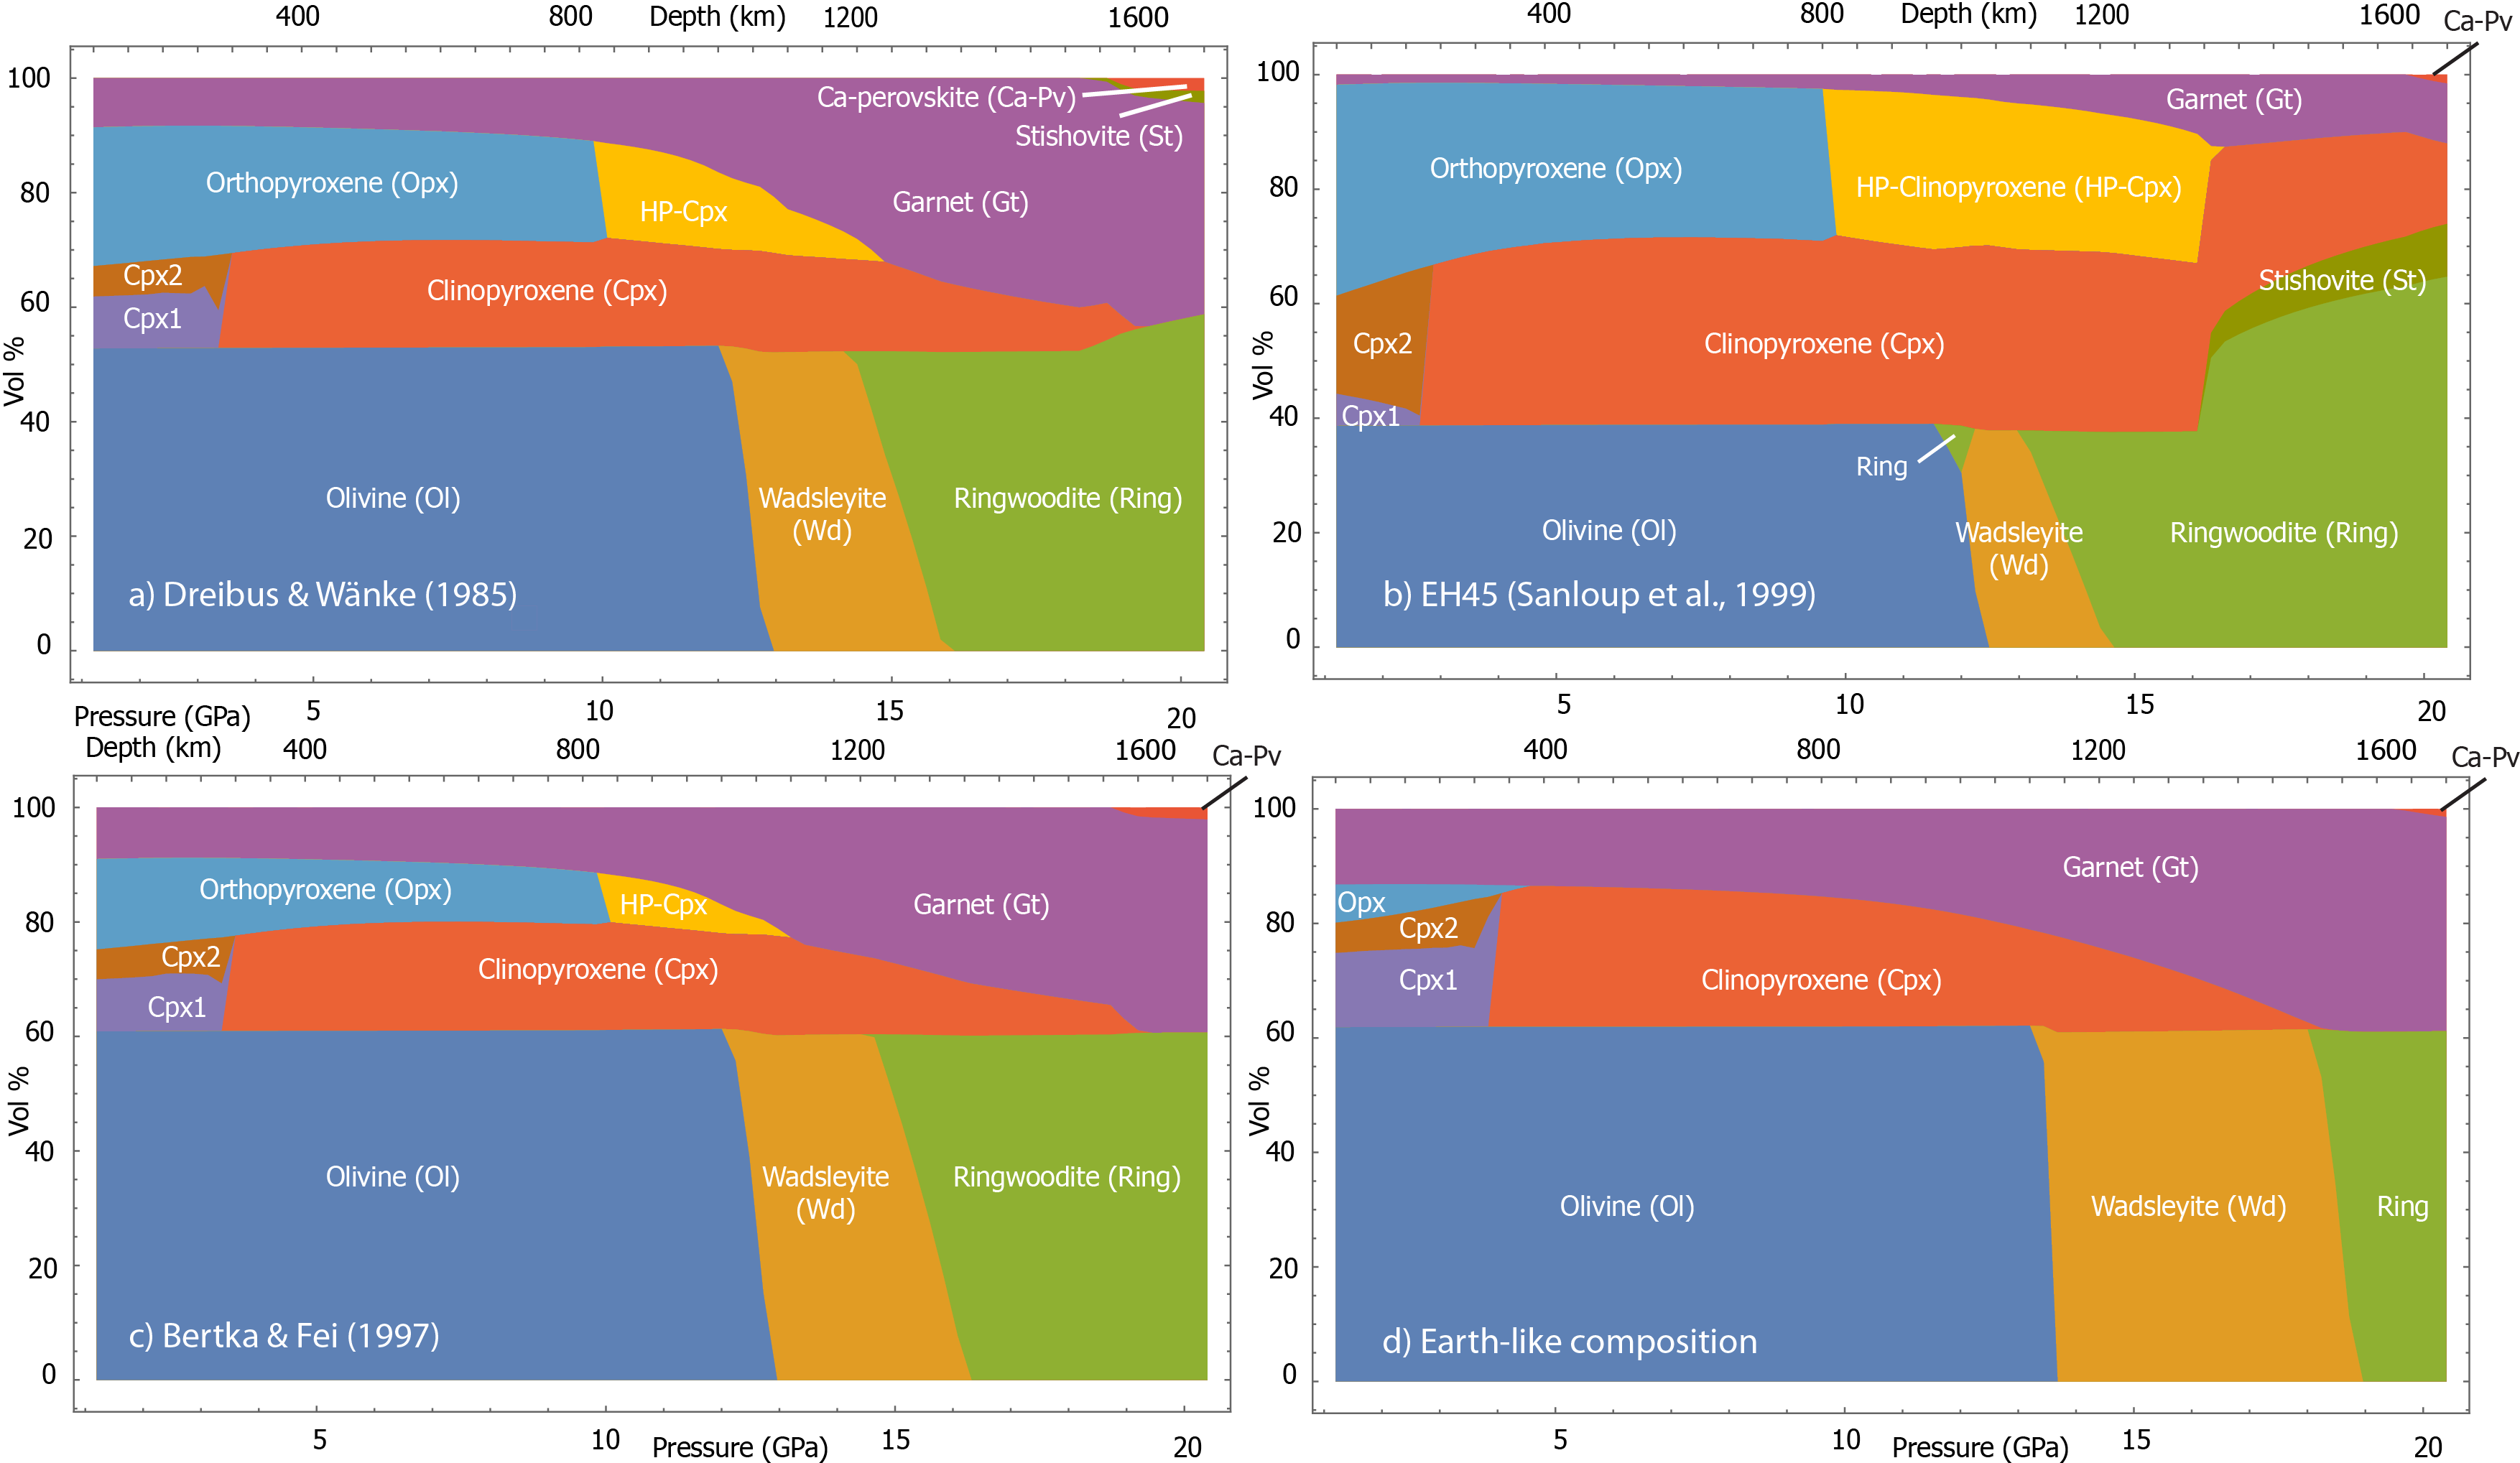
\includegraphics[width=1.0\textwidth]
{figures/Fig_Mineralogy.png}
\caption{Modal mineralogy of Mars as a function of pressure for four bulk compositions. a) Olivine-rich composition of \cite{Dreibus&Wanke1985} revised by \cite{Taylor2013}; b) Pyroxene-rich composition of \cite{Sanloup1999}; c) Modal composition synthetized by \cite{Bertka1997} at high pressure and high temperature. The iron content of the three Martian models (Fe\#0.2) is twice the Earth's mantle value (Fe\#0.1). An Earth-like pryrolitic composition \citep{Ringwood1975} is displayed in panel d) for comparison.}
\label{fig:Fig_Mineralogy.png} 
\end{center}
\end{figure}

\subsection{Gravity, Topography, and Crustal Thickness}

Models of the gravity field of Mars have been improved successively by the analysis of radio tracking data from multiple spacecraft over a time span of several decades. The most recent models (e.g., Genova et al. 2015, Goossens et al. 2017) are expressed up to spherical harmonic degree and order 120, which corresponds to a full-wavelength spatial resolution of about 178 km on the surface. The gravity field is uniquely determined by the three-dimensional distribution of mass within the planet, and thus provides information on how density varies both laterally and with depth. Interpretation of the gravity field is well known to be inherently non-unique, but by making reasonable assumptions based on geologic expectations, and by making use of the surface topography of the planet  (Smith et al. 2001) as a constraint, it is possible to invert for several properties related to the crust and lithosphere.\par
One analysis approach is to assume that Mars differentiated into a distinct crust and mantle, and that the ancient highland crust is isostatically compensated. This model predicts a relationship between the average crustal thickness, the crustal density, and the ratio of the geoid and topography (Wieczorek and Phillips 1997). Mars is divided along a hemispheric dichotomy into the heavily cratered southern highlands and the northern lowlands, where impact basins have been buried by a combination of sedimentation and volcanism. (Wieczorek and Zuber 2004) argue that the southern highlands are more likely to be isostatically compensated than the lowlands. They find that the best-fitting average thickness of the highlands crust was between 53 and 68 km for assumed crustal densities of 2700 and 3100 kg m\textsuperscript{3}, respectively. When considering the uncertainties on the geoid-to-topography ratio, the 1$\sigma$  limits of the average crustal thickness range from 39 to 81 km. The major uncertainty with this approach is that it is difficult to prove that the ancient crust is in fact isostatically compensated, and the density of the crust is highly uncertain.\par

A second modeling approach that can be made is to assume that the rigid outer portion of the planet, the lithosphere, behaves as an elastic shell when subjected to loads both on the surface and within the crust. For a given elastic thickness, these models compute the loads and lithospheric deflections that match the observed surface topography. Though these models depend upon several parameters, including the crustal thickness and mantle density, the density of the surface load is the best constrained. Localized spectral analyses applied to the large Martian volcanoes shows that the densities of the volcanic loads are close to 3200 kg m\textsuperscript{3} \citep{McGovern2004, Belleguic2005, Grott2012}. Beuthe et al. 2012), which are consistent with the densities of the Martian basaltic meteorites \citep{Neumann2004}. Only for the Elysium rise is the density of the crust beneath the volcanic load constrained in these models. For this region in the northern lowlands, the density of the underlying crust was found to be the same as that of the volcanic load itself \citep{Belleguic2005}, suggesting that the entire northern lowland crust may be largely basaltic. The elastic thicknesses obtained from these studies will be discussed in section 3.1.\par
A third modeling approach is to assume that the observed gravitational field is a result of variations in relief along the surface and crust-mantle interface. By assuming densities of the crust and mantle, as well as a mean thickness of the crust, it is possible to invert for the relief along the crust-mantle interface, providing a global crustal thickness map (e.g., \citep{Neumann2004}. This modeling approach makes no assumptions as to whether the crust is isostatically compensated or not, and in practice, the parameter values for the inversions are constrained such that the minimum crustal thickness is equal to a specified value that is greater than zero. The minimum crustal thickness of Mars is found to be located in the interior of the Isidis impact basin, which lies just south of the dichotomy boundary. One of the major uncertainties with these models is that the crustal density is not known. As shown by \cite{Baratoux2014}, the surface composition of Mars is similar to the basaltic meteorites. If these high densities are representative of the underlying crust, to obtain positive crustal thicknesses everywhere, the mean crustal thickness could be as high as 110 km (see also Pauer and Breuer 2008, who provide a maximum density of 3020 kg m\textsuperscript{3}). The minimum crustal thickness to use in these models is also unconstrained, though a value close to zero, as with the Moon (Wieczorek et al. 2013, Miljković et al. 2015), is probably a reasonable estimate. Lastly, it is likely that the density of the subsurface crust varies laterally, but these variations are not easy to constrain based on remote sensing data.

We have constructed a suite of crustal thickness models for use in modeling the seismic data that will be obtained from InSight (see also \cite{Plesa2016}). These models differ from previous studies in several ways. First, in computing the gravity field, we consider the hydrostatic deflection of density interfaces within the mantle and core using the reference density models shown in Section 3.2.3. These models consider the non-hydrostatic gravitational potential arising from the lithosphere when computing the hydrostatic interfaces, and these deflections are responsible for 3.6-5.6\% of the observed zonal degree-2 gravitational field. Second, we consider the possibility that the density of the crust in the northern lowlands is different from that of the southern highlands (e.g., \cite{Belleguic2005}). Third, we consider a wide range of crustal densities, from 2700 to 3200 kg m\textsuperscript{3}. Lastly, as their are yet no seismic constraints on crustal thickness, we use a minimum thickness constraint, where the minimum crustal thicknesses from 1 to 20 km. The thickness of the crust at the InSight landing site varies from 19 to 90 km in these models. In Figure \ref{fig:GravityTopo} , we show one such model where the crustal densities of the southern highlands and northern lowlands are 2900 and 3000 kg m\textsuperscript{3}, respectively. Data obtained from the InSight mission will constrain the crustal thickness at the InSight landing site, and will also constrain the core and mantle density profiles.

\begin{figure}[h!]
\begin{center}
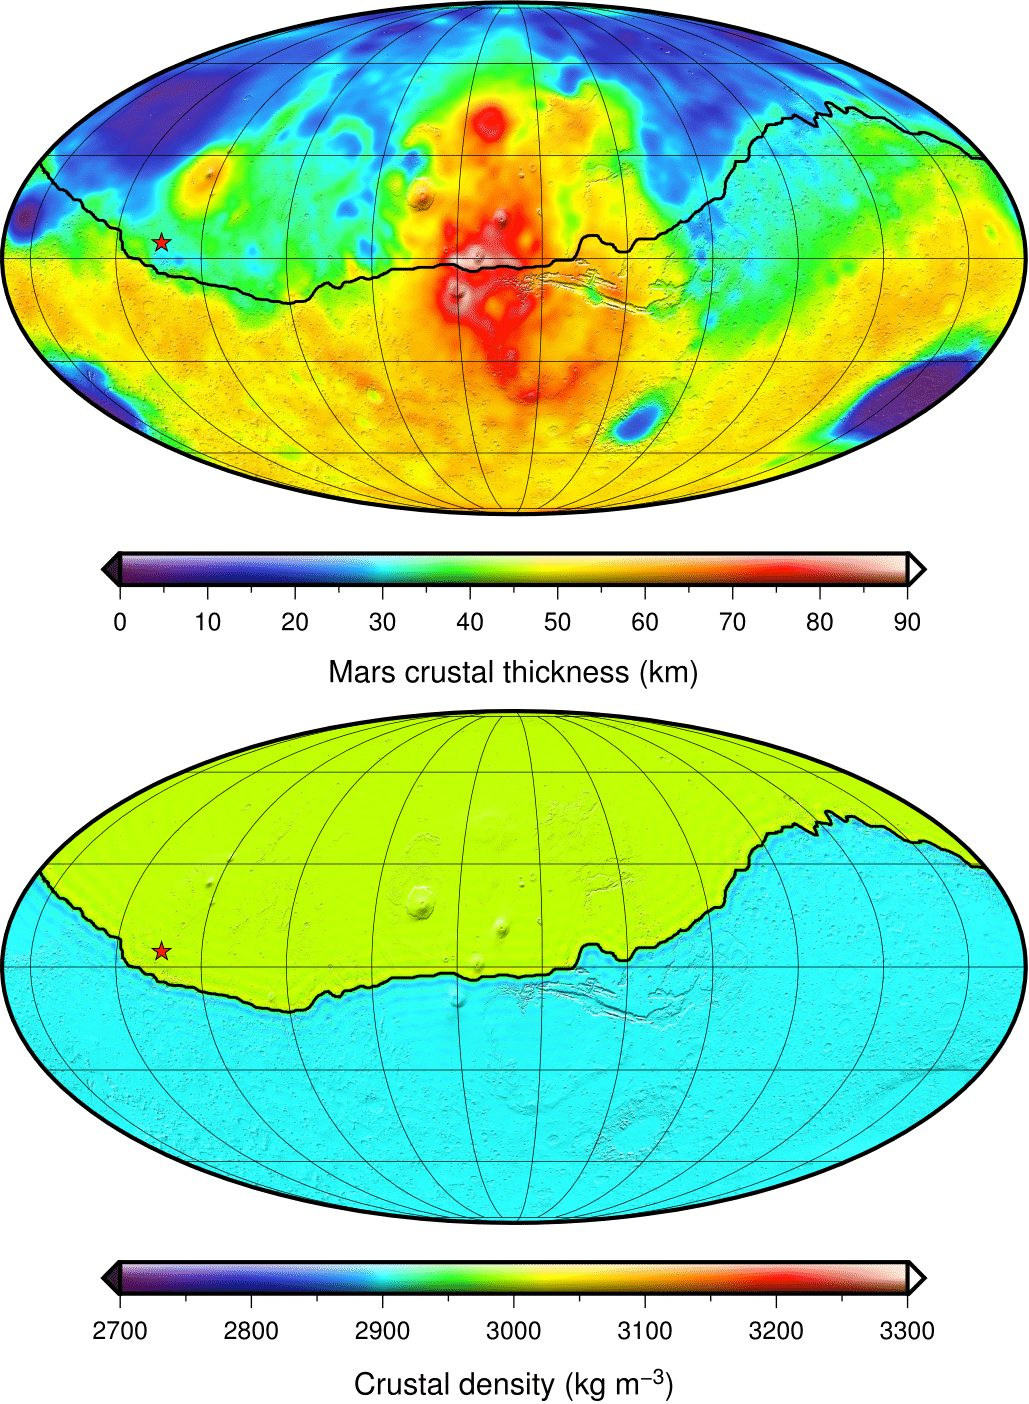
\includegraphics[width=0.65\textwidth]
{figures/GravityTopo.png}
\caption{Representative crustal thickness model (top) using the interior density profile for the model DWTh2Ref1. The crustal densities for the southern highlands and northern lowlands (bottom) are 2900 and 3000 kg m-3, respectively. The minimum crustal thickness was constrained to 1 km, which determines the average crustal thickness to be 42 km and the crustal thickness at the InSight landing site (star) to be 32 km. Data are presented in Mollweide projections centered over the Tharsis province (100° W), and grid lines are spaced every 30 in latitude and longitude. The dictomomy boundary used in the lower image is taken from \citep{Andrews-Hanna2008}}
\label{fig:GravityTopo} 
\end{center}
\end{figure}


\subsection{Constraints on the Lithosphere Thickness}

In the absence of direct heat flow measurements, temperatures in the planetary interior can be estimated from the mechanical properties of lithospheric plates. In this regard, the effective elastic lithosphere thickness Te is commonly used to describe the response of the lithosphere to loading, and given a rheological model, the mechanical thickness of the lithosphere Tm can be derived from Te. Using the yield-strength envelope formalism \citep{McNutt1984}, Tm can in turn be identified with an isotherm, and in this way estimates of planetary heat flow can be derived.

Most Te estimates for Mars have been derived from gravity and topography admittance modeling \citep{McGovern2004, Kiefer2004, Belleguic2005, Hoogenboom2006, Wieczorek2008, Grott2012}, but some geological features allow for more direct approaches. \citet{Phillips2008} have modeled the lithospheric deflection due to polar cap loading, and analysis of rift flank uplift has been used to constrain Te at the Tempe Terra, Coracis Fossae, and Acheron Fossae rift systems \citep{Barnett2002, Grott2005, Kronberg2007}. In addition, the lithospheric stress distribution due to mascon-loading at the Isidis basin has been employed to model Te using the position of the Nili Fossae circumferential graben system as model constraint \citep{Comer1985, Ritzer2009}. Other approaches estimate Te from an analysis of the depth to the lithosphere’s brittle-ductile transition \citep{Schultz2001, Grott2007, Ruiz2009,MUELLER2014100, Egea-Gonzalez2017}, but these approaches carry additional uncertainty. 

To correlate heat flow estimates with time it is usually assumed that the observed paleo-flexure corresponds to the age of the deformed surfaces, and flexure is generally assumed to be frozen-in at the time of loading. However, care must be taken when interpreting these results, as stresses in the lithosphere will decay as a function of time due to viscous relaxation and the true time corresponding to the observed paleo-flexure is generally determined by a competition between loading rate, lithospheric cooling rate, and stress relaxation rate \citep{Albert2000, Brown2000}. In this regard, the elastic thickness estimate by \citet{Phillips2008} is an exception, as the time of loading by the Martian polar caps can be tightly constrained to $<5$ Myr \citep{Phillips2008}.

Elastic thickness has increased with time \citep{GolombekM.P.andPhillips2010,Grott2013,Ruiz2014}. In the Noachian, Te was $< 20$ km. Values quickly increased to $>50$ km during the Hesperian, which can at least partially be attributed to rheological layering \citep{Burov1995, Grott2008, Grott2009}. During the Amazonian Te further increased to $40 <$ Te $< 150$ km on average, and best estimates for the present-day elastic thickness are above 150 km. In particular, the absence of lithospheric deflection due to loading at the north polar cap locally constrains present-day Te to values greater than 300 km at this location \citep{Phillips2008}. Such large present-day elastic thickness values could either imply a sub-chondritic bulk composition in terms of heat producing elements \citep{Phillips2008}, or a large degree of spatial heterogeneity of the mantle heat flow \citep{Phillips2008, Grott2009, Grott2010, Kiefer2009, Plesa2016, Breuer2016}. It is worth noting that some studies assume that the large Te determined for features on the Tharsis rise are representative for the rise itself \citep{Banerdt2000,Phillips2001}. As a consequence, Te would have been much larger and close to 100 km during the Noachian \citep{Zhong2002,Zhong2003}, and regional and global flexure models using Te = 100 km were found to be consistent with the location and orientation of tectonic features \citep{Banerdt2000} and valley networks \citep{Phillips2001}.

\subsection{Geodesy}
Planetary geodesy is one of the primary means for probing the interior structure of planets, in particular when no seismic observations are available. By radio tracking many spacecraft orbiting Mars, an accurate gravity field has been determined over the past decades. Expressed in terms of spherical harmonics, the field is now accurate up to about degree 100 \citep{Konopliv2016, Genova2016}, corresponding to a horizontal surface resolution of about 215 km. Most important for the deep interior of Mars are the lowest degrees. The degree-two components of the gravity field are related to the three principal moments of inertia of Mars, and as such inform on the mass distribution in the planet. Information on the radial density profile can be obtained from the mean moment of inertia, but this quantity cannot be determined form the gravity field alone. By complementing the degree-two components of the gravity field with precession, the mean moment of inertia of Mars has been determined and as such a first constraint on the overall mass distribution inside Mars from center to surface has been obtained.

Precession is determined from analysing radio tracking data of Martian landers and orbiters over several decades (e.g. \citep{Konopliv2011, LeMaistre2013, Kuchynka2014, Konopliv2016}. The most recent estimate of the precession rate of Mars yields a mean moment of inertia normalized by the product of mass and squared radius of Mars of 0.3639 \textpm{0.0001}, with the error mainly due to the error on the precession estimate \citep{Konopliv2016}.  Since it is an integrated quantity over the mass density in Mars, the moment of inertia, even when accurately known, cannot precisely constrain more local properties of the interior such as for example the radius of the core. Even employing the simplifying assumption that Mars were to consist of two equal density layers (the core and the mantle plus crust), the error on the core radius from the moment of inertia constraint would be several hundred km Van Hoolst and Rivoldini 2014). RISE will improve the determination of the precession rate by a factor of two but its effect on the estimate of the core radius is negligible without considering other data.

Up to now, solar tides have been the most constraining geodesy quantity for the core of Mars. Since the tidal potential is accurately known (Van Hoolst et al. 2003), the tides can be interpreted in terms of the reaction of Mars to the gravitational forcing which is very sensitive to the size of a liquid core. Tidal surface displacements have not yet been observed since their amplitude is only a few centimeters at most \cite{VanHoolst2003}, but the mass redistribution inside Mars associated with tidal deformations has an observable effect on the orbital motion of spacecraft around Mars. The tidally induced changes in the external gravitational potential of Mars are described by the Love number k2. The most recent determination of the solar tides yields k2=0.163\textpm {0.008}, based on the estimates of \cite{Konopliv2016} and \cite{Genova2016}. It implies that the radius of the core is about 1788 \textpm{73} km for the SEIS reference models (see Fig. 2.5.1). 

\begin{figure}[h!]
\begin{center}
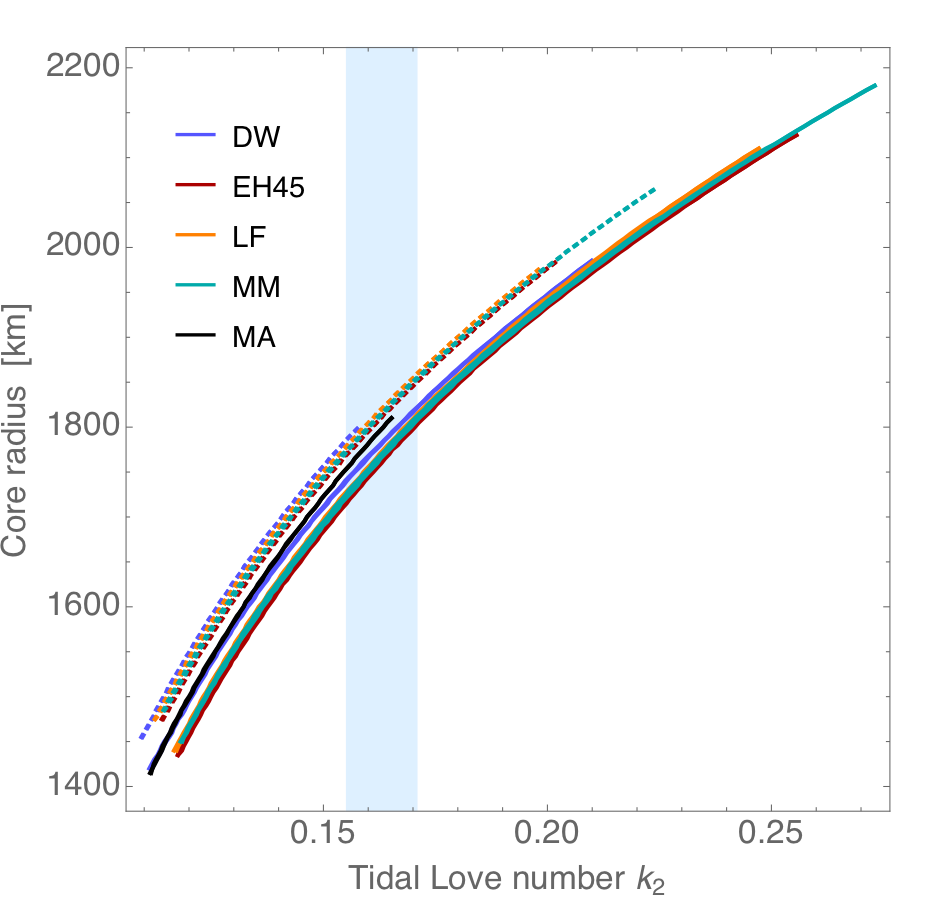
\includegraphics[width=0.65\textwidth]
{figures/Geodesytable.png}
\caption{ Core radius as a function of Love number k2 for the hot (solid curves) and cold (dashed curves) mantle temperature profile from \citep{Panning2016}.  The blue shaded area represents the range of k2 values from \citep{Konopliv2016} and \citep{Genova2016} The acronyms stand for the different mantle mineralogy models (DW: \citep{Taylor2013}, EH45: \citep{Sanloup1999}, LF: Lodders [2000], MM: \citep{Mohapatra&Murty2003}, MA: \citep{Morgan1979}. Models agree at 1$\sigma$ with the average moment of inertia of Mars (MOI=0.3639 \textpm 0.0001) \citep{Konopliv2016}.} 
\label{fig:Geodesytable.png} 
\end{center}
\end{figure}

The radio science experiment RISE of InSight will improve the estimate of precession and thus of the moment of inertia of Mars, but more importantly it will for the first time measure the effect of the core on the periodic orientation changes of Mars in space (nutations). This will allow determining  the dependence of nutation on the interior structure. In particular, it will be able to improve our knowledge on the core (see the paper of \cite{Folkner2018} in this issue).


\subsection{Crustal Magnetization and Dynamo History}
Mars has no present dynamo field but Mars Global Surveyor (MGS) data revealed a remanent crustal magnetic field that provides constraints on crustal evolution and thermal history, in particular on the existence and timing of an ancient dynamo.  There are also time-varying fields, driven by interaction of the Interplanetary Magnetic Field (IMF) with the magnetic field of Mars. They induce electrical currents in the interior that result in secondary induced fields. Magnetic sounding techniques use such time-varying magnetic fields at different periods to probe the interior electrical conductivity structure as a function of depth.  Below we discuss Mars' crustal field and its implications for Mars' thermal history. Magnetic sounding and electrical conductivity structure are discussed in Sections 3.2.2 and 3.2.3.

\subsubsection{The Crustal Magnetic Field: Observations and Models}

Systematic mapping of the martian magnetic field has been conducted by MGS (1997-2006) and MAVEN (Mars Atmosphere and Volatile EvolutioN, 2014-present), both of which measure the vector magnetic field. MGS collected data mainly at 360-440 km altitude in a 2 am/2 pm orbit.  Observations below 360 km were made over about 20\% of the surface but mostly on the dayside (magnetically noisier). MAVEN is in a highly eccentric orbit with periapsis covering a range of local times and latitudes, typically at 140-170 km altitude, but occasionally lowered to about 110 km.\par
The first crustal magnetic field maps were of data shown at satellite altitude \citep{Acuna1999, Acuna2001, Connerney2001}.  Early global models represented the magnetic field either using equivalent source dipoles [e.g., \cite{Purucker2000, Langlais2004}] or spherical harmonics [e.g., \citet{Arkani-Hamed2001, Arkani-Hamed2002, Arkani-Hamed2004, Cain2003}]; for a detailed review see \citet{Langlais2010}. Early interpretations, largely based on high-altitude measurements, indicated possible relations with tectonics patterns or signatures \citep{Connerney1999, Nimmo2000, Connerney2005}, with long, east-west aligned, magnetic field anomlies in the southern hemisphere. These were later challenged by more recent models and lower altitude maps. They include a spherical harmonic description of the field with a spatial resolution of 195 km, that is stable with respect to downward continuation to the planetary surface \citep{Morschhauser2014} and a locally higher resolution model over the martian South Pole \citep{Plattner2015}.  Electron reflectometer observations by MGS have also been used to build maps of the crustal magnetic field strength at ~170 km latitude \citep{Lillis2008}, and combined with vector data \citep{langlais2010b}.  Crustal field models differ in details, some of which may be important to interpretations (see later), but all have the same major features. The strongest fields are spatially associated with the pre-Noachian-age Terra Cimmeria and Terra Sirenum regions, crustal fields are notably absent or weak in many major impact basins and over the smoother terrain north of the hemispheric dichotomy.(See Figure \ref{fig:Magneticfield}).

The maximum spatial resolution achievable by magnetic field models depends primarily on the minimum altitude of nighttime (quiet) data. Recent MAVEN data show previously unresolved signals, especially at altitudes below ~250 km. They permit higher spatial resolution crustal field models, both because of the substantial increase in low altitude, nighttime observations and because they allow MGS measurements to be better selected by cross validation \citep{Mittelholz2016,langlais2017AGU}.

\subsubsection{Implications for crustal structure and Mars’ thermal evolution}

The strong magnetic anomalies imply large volumes of magnetized crust and/or strong magnetizations \citep{Connerney1999, Purucker2000} acquired in an ancient dynamo field.  Major, coupled questions arise, which are listed below.

(1)	How was the magnetization acquired? The canonical interpretation of the martian magnetic anomalies is that they arise from thermal remanent magnetization (TRM), acquired during cooling of crustal rocks (either new melts or reheated crust) in the presence of a global field. Another possibility is shock remanent magnetization (SRM) which has been inferred for pyrrhotite-dominated shergottite meteorites \citep{Gattacceca2004}, and shock can also result in demagnetization signatures \citep{Hood2003}. Finally, chemical remanent magnetization (CRM) due to alteration of near-surface or deep crustal rocks by water may have played an important role (e.g. \citet{Harrison2002, Quesnel2009}).  \citet{Chassefiere2013} postulated that the current martian magnetization can possibly be explained by the formation of magnetite through serpentinization, which also trapped the large volumes of water needed to carve the valley networks.

(2)	What magnetic mineral(s) carry magnetization and what is their distribution in the martian crust?  This question has been discussed extensively, however it is not possible to answer uniquely.  A constraint resides in the large magnetization magnitudes needed to explain magnetic field measurements. Single-domain magnetite and pyrrhotite-bearing carbonate were found in the meteorite ALH 84001 \citep{Weiss2002, Weiss82004, Weiss2008}.  \citet{Dunlop2005} suggested that single-domain magnetite, single-domain pyrrhotite, multidomain or single-domain hematite or a mixture of both could account for the observed strong fields. More recently \citet{Gattacceca2014} found up to 15 wt\% of iron oxides (magnetite) in meteorite NWA 7034, later altered into maghemite. 

(3)	When did Mars have an active dynamo?  The timing of initiation of the dynamo on Mars is very difficult to constrain, although the existence of remanent magnetic fields over some basins argue for a dynamo present at ~4.25 Ga. It may have started earlier, immediately after differentiation or later (e.g., \citet{Breuer2010}). The dominant view on timing of the dynamo cessation is based on early MGS observations that most of the very large basins and volcanic complex are devoid of substantial crustal magnetic fields, implying that the dynamo ceased before they were emplaced at ~4.1 Ga \citep{Acuna1999, Frey2008, Robbins2013}. The meteorite ALH 84001 has been suggested to carry a primary remanence that originated on Mars at 4.1 Ga, but possibly as late as 3.9 Ga, in a paleofield of ~50 $\mu$T \citep{Weiss2002, Weiss82004, Weiss2008}, compatible with that inferred from NWA 7034 at a similar epoch \citep{Gattacceca2014}. Remanent fields are associated with some younger, smaller impact structures, as well as volcanic plains and edifices \citep{Langlais2007,Milbury2012a}. To first order there is also a large-scale correlation between valley networks and magnetic anomalies \citep{Hood2010}. The decrease in surface activity (volcanic and aqueous), close to the Noachian-Hesperian transition, indicates a drastic change of the internal dynamics of Mars \citep{Baratoux2013, Mangold2016}. These suggest that the Martian dynamo could have persisted up to 3.7 Gy or so. The magnetic records of ~1.3 Ga nakhlites are compatible with the absence of a dynamo field at that time \citep{Gattacceca2004, Funaki2009}. An important, related issue is whether all crustal magnetization was acquired in a core field or partly in the presence of existing crustal fields \citep{Gattacceca2004}.

Early dynamos driven by thermal or thermo-chemical convection have been proposed (e.g. \citet{Stevenson2001, Lillis2008, Stanley2008}).  Later dynamos (either longer duration or delayed onset) place more restrictive constraints on the concentration of light elements (see Section 3.2.1.4) and heat-producing elements in the core \citep{Schubert2000}. The heat transport in the martian mantle has also consequences on the dynamo regime. A degree one convection pattern may have led to a hemispheric dynamo \citep{Amit2011, Dietrich2013}.  The consequences of impacts for initiating, powering and terminating a dynamo field have also been explored \citep{Kuang2008, Roberts2009, Monteux2015}.

\subsubsection{Open questions for InSight}

A major unknown from current crustal field models is the amplitude of the field at the surface of Mars.  In particular, regions such as that around InSight landing site show weak fields at ~200 km altitude (see \ref{fig:Magneticfield}) in models based on MGS data alone as well as more recent models built from MGS and MAVEN data \citep{Langlais2010, langlais2017AGU, Mittelholz2016} and suggest weak to no magnetizations directly around the landing site.  These models however cannot sense magnetizations with scale lengths smaller than the altitude of the measurements,  ~120 km or less, that could give rise to stronger surface fields than currently predicted.  With InSight, the first deployment of a magnetometer on Mars will provide us with measurements of the surface field. These will include the crustal field (if any), but also periodic and aperiodic variations due to external fields and fields due to the lander itself. Daily, quasi-monthly and annual periods have already been identified in measurements from orbit \citep{Langlais2017, Mittelholz2017}. The combination of InSight measurements with MAVEN’s  may allow separation of the time varying external field and the induced response to probe electrical conductivity structure of the crust and mantle (Sections 3.2.2 and 3.2.3).

\begin{figure}[h!]
\begin{center}
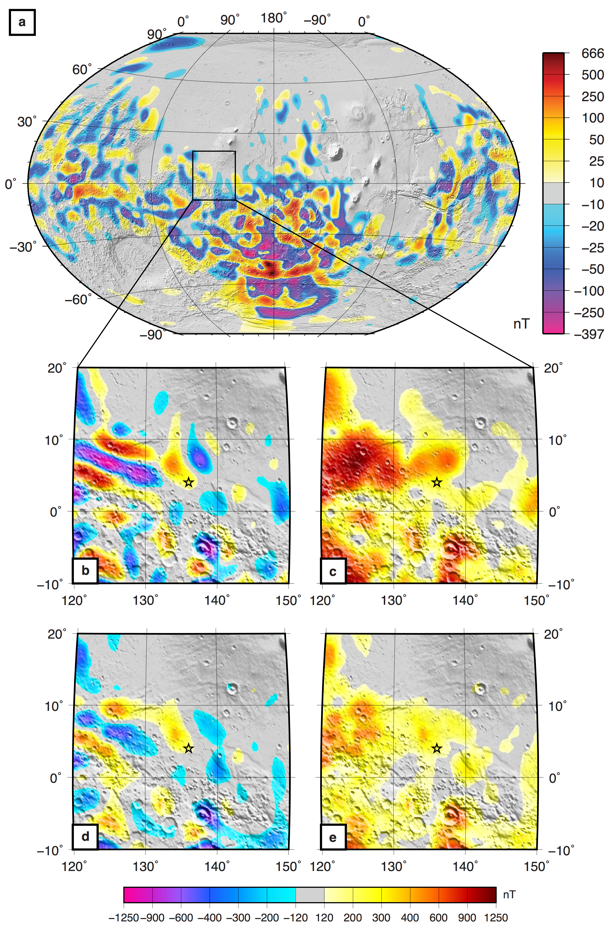
\includegraphics[width=0.8\textwidth]
{figures/Fig_6Sue.png}
\caption{(a) The radial component of the magnetic field 185 km above the planetary surface predicted by the model of \citep{Morschhauser2014}. The model uses MGS data only.  The insets (b)-(e) show two higher resolution regional model predictions for the surface field in the vicinity of the InSight landing site \cite{Langlais2017, Mittelholz2017}. Insets (b) and (d) show the radial magnetic field, $B_{r}$, and (c) and (e) the amplitude of the magnetic field, $\vert$B|, for each model respectively.  Both models use the same equivalent source dipole modeling approach and use MAVEN and MGS data.  The model in (b, c) is extracted from a global solution, and the model in (d,e) is a local solution in the vicinity of the landing site – both models agree well in overall structure.}
\label{fig:Magneticfield} 
\end{center}
\end{figure}


\newpage
\section{Models of the Interior \label{sec:models}}\subsection{Thermal History and Present Thermal State}
The thermal evolution of Mars and its present thermal state cannot be assessed by direct measurement. Rather, the thermal history needs to be reconstructed from the thickness of the crust, the timing and distribution of surface volcanism as well as the erupted volume over time, petrological and isotope data of the Martian meteorites, and estimates of the elastic lithosphere thickness. In addition, the evolution of the atmosphere and the magnetic properties of the planet need to be considered. The InSight mission will complement these data by providing a measurement of the surface heat flow at the landing site that has a good chance of being representative of the average surface heat flow \citep{Plesa2016} of the planet. Numerical model calculations of the thermal evolution and the present thermal state offer valuable insights into the interior of the planet and can be used to integrate the observational data into a coherent model. In this section, we discuss the thermal evolution of Mars and present reference models of its present thermal state.

A number of numerical studies using either parametrized models or 2D and 3D fully dynamical simulations of mantle convection have been employed to investigate the thermal evolution of Mars \citep[for a recent review see][]{BreuerMoore2015}. While the parameterized models rely on appropriate scaling laws of convective heat transport to compute average values of quantities such as temperature and crustal thickness, 2D and 3D calculations numerically solve the full set of conservation equations of mass, momentum and thermal energy. The advantage of parametrized models is that they can span a large set of parameters and initial conditions for which fully dynamical simulations may require excessive amounts of computational time. However, albeit computationally fast, parametrized models cannot self-consistently resolve spatial variations caused by e.g., mantle plumes and crust thickness variations and for this, 2D and 3D fully dynamical models are better suited.
\subsubsection{Crust formation, crust and mantle chemical reservoirs}
\label{Crust formation}
The timing of volcanic activity and amount of crustal production as well as volcanic outgassing and magnetic field history have been mostly investigated with parametrized thermal evolution models \citep[e.g.,][]{Hauck2002, Breuer2003, Breuer2006, Schumacher2006, Fraeman2010, Morschhauser2011, Grott2011} although this topic has been addressed also in 2D and 3D studies \citep[e.g.,][]{Ruedas2013, Plesa2014a, Sekhar2014}. The models predict an intense episode of mantle melting and crust formation early in the planetary evolution (i.e., during the Noachian and early Hesperian) and are consistent with the observations if a wet mantle rheology and a comparatively low initial temperature are used \citep[e.g.,][]{Hauck2002, Breuer2006, Fraeman2010, Morschhauser2011, Grott2011}. Although a dry mantle rheology with a primordial crust and higher initial mantle temperature would also be consistent with the inferred crustal history \citep{Breuer2006}, such models cannot be reconciled with the small elastic lithosphere thickness values inferred for the Noachian epoch from lithosphere deformation studies \citep{Grott2008, Grott2013}. A recent study, using 3D thermal evolution models showed that a dry mantle rheology can explain the small elastic thickness during the Noachian but in this case a wet crustal rheology must be assumed \citep{Breuer2016}. The large present-day elastic lithosphere thickness at the north pole of Mars necessarily requires a dry mantle rheology today, however. This suggests that the Martian mantle may have contained a rheologically significant amount of water, which has been partly or entirely lost by outgassing over time while  the Martian crust must have been rheologically wet at least during the Noachian period.   

The volcanic activity of Mars rapidly declined during the Hesperian and Amazonian and became restricted to the large volcanic provinces in Tharsis and Elysium \citep[e.g., ][]{Greeley1981}. Numerical studies in 3D geometry show that accounting for mantle phase transitions, a pressure-dependent viscosity or a viscosity layering in the mid mantle, possibly associated with a mineralogical phase transition in the interior of Mars, can lead to a low degree convection pattern, which may produce the observed crustal dichotomy and explain long-standing volcanic activity in Tharsis and Elysium \citep[e.g.,][]{Harder1996, Breuer1998, Zhong2001, Roberts2006, Keller2009, Sramek2010}. 
A dynamic link between the early evolution of Tharsis and the crustal dichotomy has been also suggested as a result of the formation of a thick lithospheric keel underneath the southern hemisphere \citep{Zhong2009,Sramek2012}. This lithospheric keel may represent the melt residue after the dichotomy formation process and, if sufficiently thick, cause the rotation of the entire lithosphere with respect to the underlying mantle, which explains the migration of the Tharsis volcanic center to the dichotomy boundary. However, dynamical models considering the formation of the crustal thickness dichotomy and Tharsis investigate only the first billion year of thermal history, and whether such models will continue to experience significant volcanic activity thereafter is still not clear. A significant amount of melt produced during later stages of evolution would be inconsistent with estimates of the crustal production rate on Mars \citep{Greeley1991}.

Models of mantle convection in 2D and 3D geometry are also a natural choice for studies of the interior dynamics of Mars, which investigate the formation and stability of geochemical reservoirs, as suggested by the isotopical analysis of Martian meteorites \citep[e.g.,][]{Jagoutz1991}. Although previous studies argued for the formation of mantle reservoirs during the crystallization and subsequent overturn of a global magma ocean \citep[e.g.,][]{Elkins-Tanton2003, Elkins-Tanton2005}, recent studies suggest that such heterogeneities could have been largely or even entirely erased if solid-state mantle convection started before the complete crystallization of the magma ocean \citep{Maurice2017}. Alternative scenarios suggest that the formation of mantle geochemical anomalies could be explained by partial melting of an initially homogeneous mantle, if additional effects like density variations and mantle dehydration are considered \citep[e.g.,][]{Schott2001, Ogawa2011, Plesa2014a, Ruedas2017}. As the planet cools, the stagnant lid (i.e., the immobile layer that forms at the top of the convecting mantle due to the strong temperature dependence of the viscosity) grows. Geochemical reservoirs if located close to the surface, may become trapped within the stagnant lid and remain protected from mixing and homogenization that otherwise would take place in a vigorously convecting mantle \citep[e.g.,][]{Breuer2016}. If on the other hand, the liquid magma ocean rapidly crystallized and no mixing took place prior to complete solidification, numerical modeling studies suggest that the density contrasts established during magma ocean crystallization would be too strong to allow the later onset of thermally driven convection \citep{Tosi2013, Plesa2014}. Such a scenario is at odds with the volcanic history on Mars and also with the thin elastic lithosphere of about 20 km inferred for the Noachian epoch (see below), which requires a thin thermal boundary layer and consequently a vigorously convecting mantle at that time.

\subsubsection{Radiogenic Element distribution in crust, mantle and core}
The long-lived radiogenic isotopes (K, Th, and U) are the primary sources of heat in the interior of Mars. Estimates of their concentrations in the primitive mantle come from geochemical models \citep[][see also section 2.2]{Dreibus1984, Wanke1994, Treiman1986, Morgan1979, Lodders1997}. Most compositional models predict similar amounts of Th but substantially different potassium abundances. Only the model by \citet{Morgan1979} has almost twice as much Th and a significantly smaller amount of K. In addition, they used a low ratio of K/U of 2200 as determined from gamma spectrometric analysis performed by the Soviet orbiter Mars 5. This value was later corrected by the gamma-ray spectrometer (GRS) data obtained by Mars Odyssey. The surface ratio of K/Th measured by the GRS instrument varies for 95\% of the surface area between 4000 and 7000 \citep{Taylor2007} and is largely consistent with the preferred compositional model of \citet{Wanke1994}.  Today the heat sources are not homogeneously distributed in the Martian interior because these incompatible elements are preferentially sequestered into a planet's crust during differentiation \citep{Taylor2008}. Alternatively, \citet{Kiefer2003} argues that recent volcanism could be driven by radiogenic material in the mantle. To estimate the abundance in the crust, in-situ measurements by landers and rovers, remote measurements from orbiting spacecraft, and meteorite samples have been used \citep[e.g.,][]{Taylor2007}
\begin{table}[h!]
\centering
\label{table2}
\resizebox{\textwidth}{!}{
\begin{tabular}{llllll}
                              & U (ppb) & Th (ppb) & K (ppm)  & H\textsubscript{0} (pW/kg) & H\textsubscript{today} (pW/kg) \\
Model                         &         &          &          &            &                \\
Treiman et al. (1986)         & 16      & 64       & 160      & 17         & 3.7            \\
Morgan and Anders (1979)      & 28      & 101      & 62       & 21         & 5.6            \\
Wänke and Dreibus (1994)           & 16      & 56       & 305      & 23         & 4.1            \\
Lodders and Fegley (1997)     & 16      & 55       & 920      & 49         & 6.2            \\
Basaltic Shergottites*+       & 26--184  & 100--700  & 200--2600 & --      & 5.9 -- 45.5     \\
GRS data                      & 163     & 620      & 3300     & --         & 49             \\
(average surface abundances)* &         &          &          &            &               
\end{tabular}
}
\caption{Abundance of heat-producing elements in the primitive mantle for various compositional models, SNC meteorites and average surface crustal composition measured by GRS and corresponding heat production at the beginning of the evolution (H\textsubscript{0}) and after 4.5 Ga (H\textsubscript{today}). *The U abundances are determined by assuming a Th/U ratio of 3.8, a canonical cosmochemical value thought to be representative of most planetary bodies and that also agrees with analyses of most Martian meteorites \citep{Meyer2003}.+ Most of the basaltic shergottites show values close to the lower bound.}
\end{table}

The GRS data do not present evidence for significant large-scale geochemical anomalies \citep{Hahn2011} and the surface distribution of Th only shows slight variations between 0.2 and 1 ppm \citep{Taylor2007}. Assuming the compositional model of Dreibus and W\"anke and further assuming that the composition of near surface rock reflects the average crustal composition, thus neglecting any intracrustal differentiation, the percentage of heat producing elements (HPE) in the crust is between 29\% and 70\% of the total \citep{Taylor2007}.  The uncertainty in this estimate is being caused by the unknown crust thickness (see section 2.3). This estimate further implies that most of the Martian crust was derived from an undepleted mantle and that the concentrations of K and Th in the bulk crust are higher than in the basaltic Martian meteorites (see Table 2) and in the basaltic rocks analyzed by the MER rovers \citep[e.g.,][]{ McLennan2001}. The latter rock samples would then need to have been derived from a depleted mantle. An alternative scenario is that a significant portion of the crust does consist of basaltic rocks relatively low in K and Th, similar to the Martian meteorites, and that the observed soil composition represents a reservoir enriched in incompatible elements relative to the bulk of the basaltic crust. In that case, the surface composition from the GRS data represents an upper limit to the abundance of HPE in the crust \citep{Newsom2007}. Assuming the W\"anke-Dreibus abundance, this would imply that only about 10\% of Th and K are partitioned into the crust, or that bulk Mars has lower abundances of Th and K.  Thermo-chemical evolution models favor the former model as this will better explain the inferred large elastic lithosphere thickness at the north pole and the recent volcanic activity (\cite{Kiefer2003}, also see section 3.1.3). 

The distribution of HPE in the mantle is basically unknown. Often, it is assumed that HPE are homogeneously mixed due to mantle convection. However, mantle melting and differentiation may lead to reservoirs of varying abundances and in particular the lower part of the stagnant lid and/or an upper mantle layer can be depleted in HPE in comparison to the lower mantle \citep{Ruedas2013, Plesa2014a}. 
The compositional models generally assume no radiogenic heat sources in the core. However, this is controversially discussed because recent experimental results suggest that K may partition into the core at the relatively low pressures and high sulfur contents appropriate to Mars \citep{Murthy2003}.

\subsubsection{Surface heat flow and the Urey ratio}
\label{Te_heat_flow_Urey}



Models of thermal evolution in a 3D geometry employing a crustal thickness whose spatial variations are consistent with gravity and topography data \citep[e.g.,][]{Neumann2004} and a crustal enrichment that matches the surface abundance of heat producing elements \citep{Taylor2007, Hahn2011} indicate elastic thickness values close to 300 km at the north pole and as small as 42 km in Arsia Mons (Figure 7a). Such low values suggest that a decoupling layer in the lower crust is still present today in this region \citep{Grott2010, Plesa2016}. The low elastic thicknesses during the Noachian period can be explained if a weak crustal rheology is assumed \citep{Grott2008, Breuer2016}. The evolution of the elastic lithosphere thickness predicted by the 3D thermal evolution models, accounting for a weak crustal rheology and mantle plumes, is shown in Figure 7b. These models show a spatial distribution of the surface heat flow, which is dominated by the crustal thickness pattern \citep{Plesa2016} and attains the smallest values in regions covered by a thin crust (e.g., Utopia, Hellas, Agyre and Isidis impact basins), while the largest values are obtained for regions covered by a thick crust (e.g., Tharsis province). A crustal thickness dichotomy leads to higher surface heat flow values for the southern highlands compared to the northern lowlands. If instead the crustal thickness variations are reduced by assuming a variable crustal density, the surface heat flow shows a rather homogeneous distribution \citep{Plesa2016}. The signature of mantle plumes may become visible on the surface heat flow maps if an activation volume of 10 cm$^3$/mol is considered, which leads to a strong increase of viscosity with pressure of about two orders of magnitude. Nevertheless, for a variety of parameters, the models predict that the location of mantle plumes is unlikely to affect the heat flow measurement. The difference between the heat flow value that will be obtained by the HP$^3$ instrument and the average surface heat flow will be less than 5 mW/m$^2$ \citep{Plesa2016}. This suggests that InSight will return a representative value for the average surface heat flow.

\begin{figure}[h!]
\begin{center}
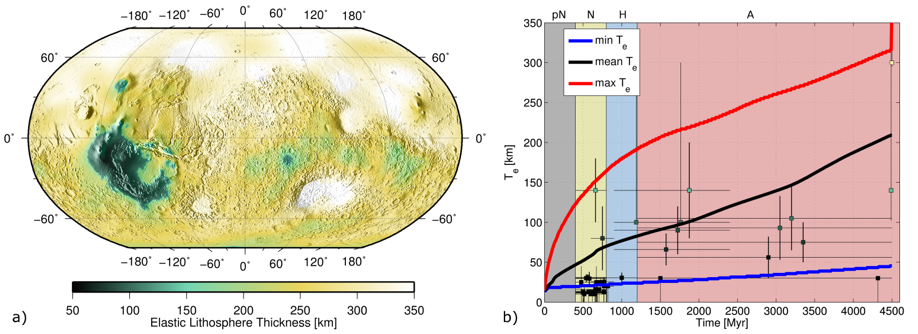
\includegraphics[width=\textwidth]
{figures/Fig3.png}
\caption{Elastic lithosphere thickness: a) Spatial distribution of the present-day elastic lithosphere thickness calculated using a strain rate of $10^{-14}$ s$^{-1}$ which is characteristic for the timescale associated with the polar cap deposition at the north pole of Mars; b) Evolution of the elastic lithosphere thickness that was computed assuming a strain rate of $10^{-17}$ s$^{-1}$, which is representative for convection timescales, for the entire evolution apart from the maximum value today. The latter has been calculated using the strain rate value of $10^{-14}$ s$^{-1}$. The colored boxes represent the elastic lithosphere thickness estimates with their corresponding error bars.}
\label{fig:Fig3.png} 
\end{center}
\end{figure}

The average surface heat flow is an important quantity which can be directly related to the bulk abundance of HPE in the silicate part of the planet (mantle and crust) by using the so-called Urey ratio, which is defined as the ratio between the heat produced by radioactive elements in the silicate part and the heat loss over the surface. Numerical simulations show that as long as the mantle of Mars is efficiently convecting, the Urey ratio converges towards a similar present-day value independent of mantle parameters such as e.g., initial mantle temperature and the distribution of heat sources between crust and mantle \citep{Grott2012a, Plesa2015}. Thus by using the average surface heat flow, which will be derived from the InSight measurement, together with the Urey ratio, that is calculated from thermal evolution models, one can estimate the bulk abundance of HPE in the interior of Mars and answer the fundamental question as to whether the amount of heat producing elements in the interior of the planet is \revision{similar to previously proposed geochemical models \citep{Wanke1994,Lodders1997,Treiman1986} or lower \citep{Phillips2008}.}

\subsubsection{Reference Temperature Profile -- A Geotherm }
\label{ref_temp}
In this section we will present a reference thermal model for the interior of Mars based on the mantle convection calculations discussed above. The 3D calculations have been introduced elsewhere in greater detail \citep[e.g.,][]{Plesa2016} and will therefore only be briefly described here. The calculations are based on the extended Boussinesq assumption \citep[e.g.,][]{Schubert2001} for which the temperature and pressure dependencies of material parameters are accounted for in the buoyancy term and for which adiabatic and viscous heating are included. In addition, the models use a pressure- and temperature-dependent rheology, with a reference viscosity evaluated at 3 GPa and 1600 K. The calculations assume a crust that has been differentiated from the mantle. We use the \citet{Neumann2004} crustal thickness model as well as other models as discussed in section 2.3 derived from MGS gravity measurements. The crust is enriched in radiogenic elements as compared to the mantle. The enrichment factor is 10 with respect to the bulk value and is consistent with the surface concentrations measured by the gamma ray instrument on board Mars Odyssey \citep{Taylor2007, Hahn2011}. The concentration of the radiogenic elements is considered constant for simplicity although it has long been argued that it may vary with depth \citep[e.g.,][]{Newsom2007}. In addition to the 3D temperature in the mantle and crust, the model provides maps of the elastic thickness of the lithosphere and the surface heat flow. Table 3 summarizes parameter choices made for the model. Note that we do not include a detailed model of the core. The likely low viscosity of the core precludes the use of a code tailored for mantle convection to model core flow. Rather, we solve an energy balance for the core in which the time rate of change of the core internal energy is balanced by the heat flow into the mantle integrated over the core surface and we extend the temperature from the core-mantle-boundary (CMB) into the core assuming a heat conduction profile discussed below. 
%

\begin{table}[h!]
\caption{Parameters used for the end-member models and the reference model. All models assume a core size of 1700 km and hence include only the exothermic phase transitions from $\alpha$ to $\beta$-spinel and $\beta$ to $\gamma$-spinel but no endothermic phase transition from $\gamma$-spinel to perovskite. \revision{All models use an activation energy of 300 kJ/mol. }For additional parameters we refer the reader to \citep{Plesa2016, Plesa2015} and \citep{Breuer1998}.}
\label{table:end_member_ref_models}

\begin{tabular}{ p{11em} p{2.5cm} p{2.5cm} p{2.5cm} }
\hline
\multirow{3}{12em} & Hot end-member model & Cold end-member model & Reference model \\
\hline 
Planetary radius {[}km{]} & 3400     & 3400    & 3400\\
Core radius {[}km{]} & 1700 & 1700 & 1700  \\
Reference viscosity {[}Pa s{]} & 1021 & 1020 & 1021 \\
Activation\_volume {[}cm$^3$/mol{]} & 0 & 10 & 10 \\
Crustal thickness model & {[}Neumann et al., 2004{]} & 3200\_1\_DWTh2Ref1 & 3100\_1\_DWTh2Ref1 \\
Depth of $\alpha$ to $\beta$-spinel 
phase transition {[}km{]}  & 1020 & 1020 & 1020 \\
Depth of $\beta$ to $\gamma$-spinel
phase transition {[}km{]} & 1360 & 1360 & 1360   
\end{tabular}
\end{table}

\revision{
The thermal models discussed below do not self-consistently account for Tharsis formation. The latter could have been formed by a low degree convection pattern \citep[e.g.,][]{Zhong2001,Roberts2006,Zhong2009,Sramek2010} or a large-scale impact onto the southern hemisphere followed by a degree-1 convection pattern \citep[e.g.,][]{Golabek2011,Golabek2018}. Whether the amount and distribution of crust produced in such scenarios would be compatible with the range of crustal thicknesses derived from gravity and topography data is still not clear. Since most of the martian crust has formed during the first 500-700 Myr of evolution \citep[e.g.,][]{Greeley1991}, the crustal thickness pattern and the crustal enrichment in heat producing elements could have influenced the underlying temperature distribution over several Gyr. By combining crustal thickness variations derived from gravity and topography data with thermal evolution models of interior dynamics and taking into account a number of observational data sets, we discuss a range of temperature variations that could be representative for the present-day interior of Mars.}

The crustal thickness pattern and the crust radioactivity cause spatial temperature variations in the shallowest layers, while deeper in the mantle thermal anomalies reflect the mantle flow pattern, which -- in turn -- is sensitive to the pressure and temperature dependence of the viscosity. \revision{The temperature and pressure dependence of the viscosity are determined by the activation energy and activation volume, respectively, and uncertainties of the activation parameters lead to uncertainties of temperature variations in the mantle. In particular, the large range of values obtained from deformation experiments of upper mantle rocks for the activation volume, i.e., 0--10 cm$^3$/mol for diffusion creep and even larger for dislocation creep \citep{Hirth2003}, indicate an increase of viscosity with pressure ranging from 0 to several orders of magnitude for Earth's upper mantle \citep{King2016} and would lead to significantly different convection planforms}. A strong increase of viscosity with pressure induces a long wavelength convection pattern with prominent mantle plumes that can considerably affect the temperature distribution and locally vary the thickness of the thermal boundary layer \citep[e.g.,][]{Yoshida2006, Roberts2006, Bunge1996}. 

On the other hand, a comparatively mild increase of viscosity with pressure, leads to weaker thermal anomalies in the mantle and smaller perturbations of the thickness of the thermal boundary layer and hence smaller overall temperature variations (compare Figs. 8 and 10 below). Temperature variations are strongest at the base of the upper thermal boundary layer, where cold thermal instabilities originate and hot mantle plumes, rising from the core-mantle boundary, locally penetrate and erode the stagnant lid. Even for the weakest thermal anomalies, temperature variations in the lithosphere are around 200 K. Recent deformation experiments conducted at pressure and temperature conditions relevant to the mantle of Mars seem to favor an increase of the viscosity with pressure through the mantle of more than two orders of magnitude \citep{Raterron2017}, thus suggesting strong mantle plumes and variations of the lithosphere temperature by several hundred Kelvin.

In Figure 8, we present two end-member models showing the smallest and largest temperature variations as well as a reference model, to be discussed further below. Figure 8 gives slices of the temperature field for the reference and end-member models using a Robinson projection at depths of 50 km (in the upper lithosphere) to 1400 km (roughly 300 km above the CMB). The models have been selected from a large number of study cases discussed in \citet{Plesa2016}. The model with the smallest temperature variations (case 8 of \citet{Plesa2016}) has no pressure dependence of the viscosity and uses the crust thickness model of \citet{Neumann2004} (Fig. 8a). The crust density is 2900 kg/m$^3$ and the minimum thickness is 5 km in the Isidis basin while the average crust thickness is 45 km. In contrast, the largest temperature variations (Figure 8b) are obtained for a model (case 27 of \citet{Plesa2016} with a strong pressure dependence of the viscosity and using the crustal thickness model 3200\_1\_DWTh2Ref1 of \citet{Plesa2016}. The crust density is 3200 kg/m$^3$, the minimum crustal thickness is 1 km in Isidis, and the  average crustal thickness is 87 km for this model. 
%
\begin{figure}[h!]
\begin{center}
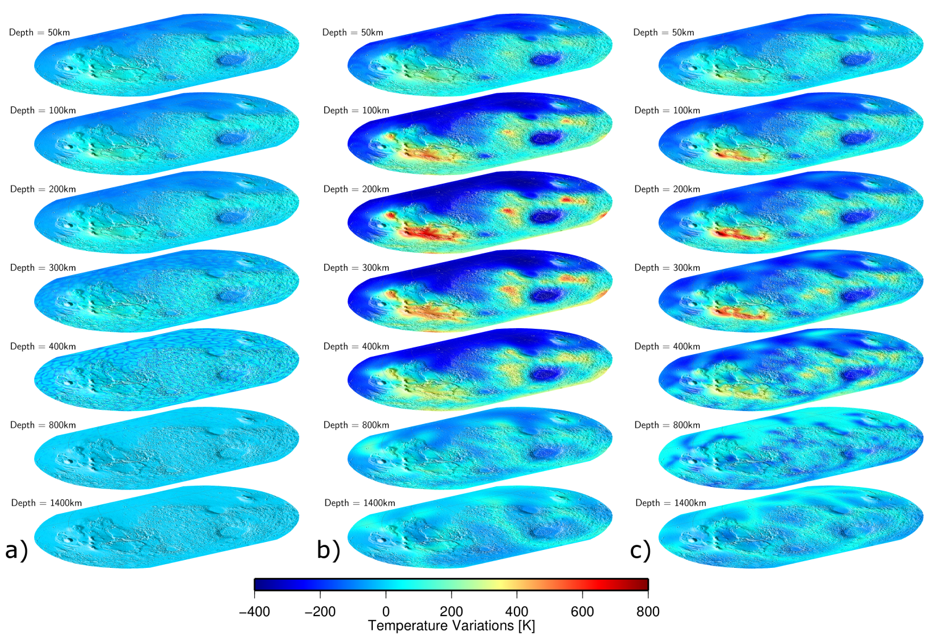
\includegraphics[width=\textwidth]
{figures/Fig4.png}
\caption{Present-day temperature variations in the Martian mantle: a) An end-member case showing the smallest variations (case 8 of \citet{Plesa2016}); b) An end-member case showing the largest variations (case 27 of \citet{Plesa2016}); c) The reference case (see text for details).}
\label{fig:Fig4.png} 
\end{center}
\end{figure}
%
The reference model has been selected by comparing our model results to a number of constraints from the Martian geologic record. As constraints we use the following observations: 
\begin{itemize}
\item	The present-day elastic thicknesses of the north and south polar lithosphere of more than 300 km and 110 km, respectively, as discussed above. In addition, the model is required to satisfy a Noachian elastic lithosphere thickness of 20 km \citep[][and references therein]{Grott2013} 
\item	Evidence for recent magmatic activity. Thus temperatures in the upper mantle must at least locally allow for partial melting. For the solidus of the mantle we use a recent compilation based on mineralogical models of the Martian mantle and available laboratory solidus temperatures \citep{Ruedas2017}.
\item	Petrological investigation of shergottites require potential temperatures in the mantle between 1480 and 1550°C around 180 -- 472 Myr ago \citep{Filiberto2015}. This observation constrains the mantle temperature to allow for at least local values in excess of the solidus temperature at the indicated times. 
\item	The potential of a model to relate the prominent topography features such as Tharsis and Hellas to mantle up- and downwellings

\end{itemize}

The model that best fits the constraints above, employs a large pressure dependence of the viscosity and a relatively thick crust. Other model parameters are taken from case 25 of \citet{Plesa2016}. The crust thickness model is 3100\_1\_DWTh2Ref1, with a crustal density of 3100 kg/m$^3$, a minimum crustal thickness of 1 km in the Isidis basin, and an average crustal thickness of about 62 km (Section 2.3). 

It can be seen that the maximum positive thermal anomalies are associated with Tharsis in both the reference and the end-member model with the largest temperature variations \revision{(Fig. 8)}. The particular thick and warm crust there that will attract mantle plumes causes this. Similarly, thin and cold regions of the crust, in particular Hellas, attract cold downwellings of mantle flow. Mantle plumes underneath Tharsis and Elysium are, of course, reasonable given the volcanic activity there that has lasted until recently \citep[e.g.,][]{Werner2009}. The figure also illustrates how the amplitudes of the thermal anomalies decrease with depth \revision{(Fig. 8)} to almost vanish near the CMB \revision{(Fig. 10)}.

\revision{In Figure 9 we show the present-day convection pattern obtained below Tharsis and Elysium in the reference model. }The model suggests that mantle plumes are present in the interior of Mars and are causing large spatial variations of the elastic thickness, surface heat flow and lithospheric temperatures (Figure 7 and 8). Large temperature variations may affect the seismic velocities in the shallowest layers of the planet up to 400 -- 500 km depth and hence may be detected by the SEIS instrument.
%
\begin{figure}[h!]
\begin{center}
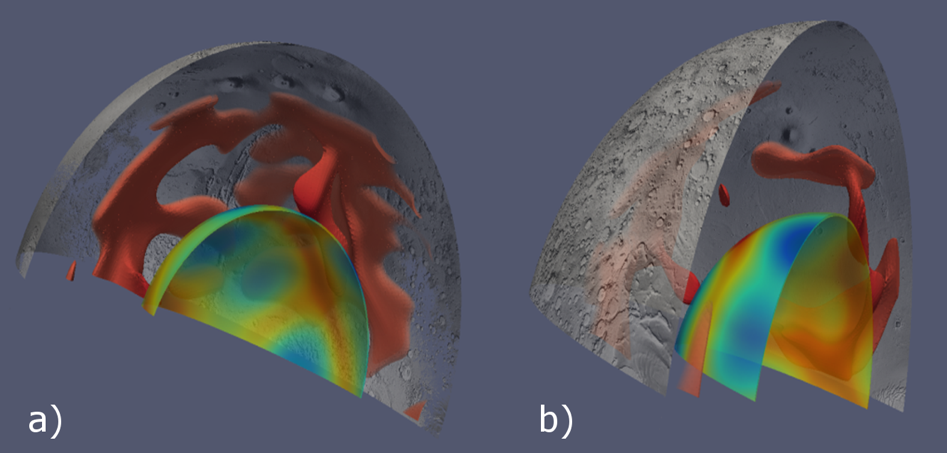
\includegraphics[width=\textwidth]
{figures/Fig5.png}
\caption{Present-day convection pattern in the interior of Mars: mantle plumes distribution below Tharsis (a) and Elysium (b) in the reference 3D thermal model.}
\label{fig:Fig5.png} 
\end{center}
\end{figure}
%

Figure 10a shows the reference temperature profile calculated from averaging over longitude and latitude at constant radial distance from the center in addition to profiles for the maximum and a minimum temperature anomaly cases introduced above. The models give the same surface heat flow value of about 24 mW/m$^2$ and a thermal lithosphere thickness of 450 to 600 km, respectively. In the thermal lithosphere, heat transfer is mostly by heat conduction and the temperature profile is comparatively steep. In the deeper mantle, the temperature profile bends over and is close to an adiabat at larger depth. For comparison, we present a mantle adiabat following \citet{Khan2018} that includes temperature jumps at mineralogical phase change boundaries. 

The deviations from the adiabat\revision{, which are observed in Figure 10a for temperature profiles obtained by 3D thermal evolution models,} are typical for convection cases with a relatively low Rayleigh number between 10$^4$ -- 10$^5$ (values computed using the average viscosity at the base of the stagnant lid \revision{at present day}) and for pressure dependent viscosity which results in a more sluggish convection in the lower mantle. \revision{We note that the initial Rayleigh numbers (i.e., calculated at the beginning of the thermal evolution) are of the order of 10$^7$ -- 10$^9$, but decrease as the interior cools and the mantle viscosity increases \citep[][Table 6]{Plesa2016}.} 

\revision{In Figure 10a,} the model with the largest temperature variations defining a cold end-member model \revision{shows} a thermal boundary layer at the CMB of about 150 km thickness with a temperature difference across of roughly 100 K and a core-mantle heat flow of 2.8 mW/m$^2$. Lower thermal boundary layers are lacking for the reference and the hot end-member models (with the smallest temperature anomalies). In both cases, the mantle has removed any initial super heat of the core during the thermal history. The heat flow from the core in both models is small (1.4 and 1.7 mW/m$^2$, respectively), certainly in all our models smaller than the heat flow along the core adiabat of at least 5 mW/m$^2$ \citep{Nimmo2000}. Thus, the models are consistent with a stably stratified core lacking a thermally driven dynamo. Finally, we note that our maximum temperature model is close to the model of \citet{Zharkov2009} in the lower mantle but has significantly lower temperatures in part of the upper mantle and a thicker thermal lithosphere. 
%
\begin{figure}[h!]
\begin{center}
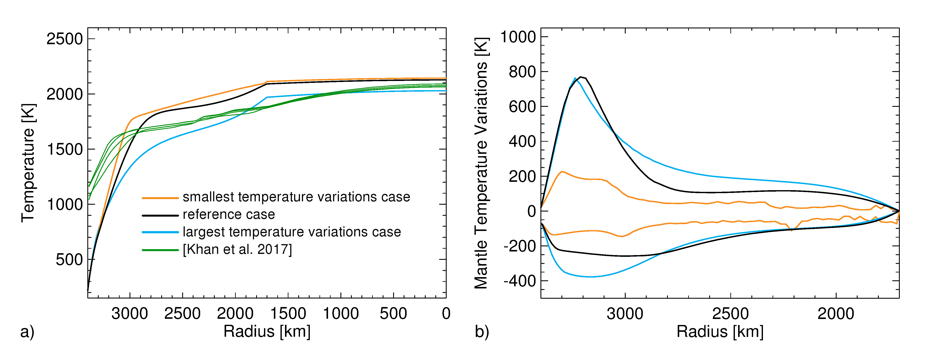
\includegraphics[width=\textwidth]
{figures/Fig4ab.png}
\caption{Panel a: temperature profiles in the mantle and core for the thermal evolution case showing the smallest temperature variations (case 8) shown in yellow color, for the thermal evolution case showing the largest temperature variations (case 27) shown in blue color and the reference case (shown in black). The temperature profiles from \citet{Khan2018} have been computed using various mantle compositions (DW, TAY, SAN and LF); Panel b: the corresponding temperature variations within the mantle as calculated from the 3D thermal evolution models by computing the difference to the average mantle temperature. Negative values indicate cold downwellings while positive values show the temperature anomaly introduced by mantle plumes.}
\label{fig:Fig4ab.png} 
\end{center}
\end{figure}
Figure 10b gives the temperature variations in the 3D calculations from the average as a function of radial distance from the CMB for the reference and the end-member models. It can be easily seen that the hot end-member model has the smallest lateral temperature variations. Upwelling and downwelling plumes are not particularly prominent. This is different for the reference model and also for the cold end-member model which both show qualitatively similar lateral variations in temperature that can reach up to 800 K at the maximum. The maxima occur partly within the thermal lithosphere. But it should be noted that the latter varies in thickness according to temperature and is comparatively thin where the temperature is large. The thermal lithosphere thickness of the reference model varies between 200 km above hot mantle plumes and up to 600 km above cold downwellings, and shows an average value of about 500 km thickness. 

The temperature of the core is little constrained. Previous models of the interior structure \citep[e.g.,][]{Sohl1997, Bertka1997, Hauck2002, Williams2004, Fei2005, Rivoldini2011, Khan2018} have assumed that the core is largely adiabatic. This would be true if the core would be vigorously convecting in which case the temperature increase in the core from the CMB to the center would amount to 200 – 300 K \citep[e.g.,][]{Sohl1997, Rivoldini2011}.  An adiabatic core will require the mantle to remove heat at a rate of at least equivalent to the heat flow conducted along the core adiabat of 5 to about 20 mW/m$^2$ \citep{Nimmo2000}. Alternatively, if the core is stably stratified, it will most likely be subadiabtic with a conductive temperature profile that matches the heat flow out of the core and the CMB temperature and has a zero heat flow in the center. We do not expect any core crystallization because core temperatures for all models are higher than the liquidus of the assumed core composition (see section 2.1).  

Our core temperature profiles assume the core to be stably stratified and are calculated to match the CMB heat flow from the detailed mantle convection calculations. In particular, 
%
\begin{equation}
T(r)=T_{CMB}+\frac{q_{CMB}}{2k_c}\left(R_c^2-r^2\right)
\end{equation} 
%    
where $T$ is temperature, $r$ radial distance from the center, $T_{CMB}$ the temperature at the CMB,  $q_{CMB}$ the heat flow there, $k_c$ the core thermal conductivity (40 W/m K) and $R_c$ the core radius. Equation (1) uses a stationary model with the cooling rate as a heat source and is a good approximation for slow secondary mantle cooling. The temperature in the core increases from the CMB to the center by some tens of Kelvin but less than 100 K. 

\newpage
\subsection{{Interior structure and composition\label{sec:interior}}}\subsubsection{Link between geophysical parameters and mineralogy and temperature}
\label{sec:geo_min_link}

In order to predict the seismic properties of Mars' mantle, equations of state must be formulated that describe the pressure- and temperature-dependence of the bulk modulus, shear modulus and density. The basis for most equations of state is a relationship between pressure and elastic constants at room temperature, for which a variety of high pressure formulations exist \citep[e.g.][]{Stacey2004}. One of the most popular is the Birch-Murnaghan (BM) finite-strain theory \citep{Murnaghan1944,Birch1952}, in which the Eulerian elastic strain energy is expanded as a Taylor series. A third-order expansion is reasonably accurate when pressures are a small fraction of the zero-pressure bulk modulus \citep{Stixrude2005}. Most endmembers of mantle minerals have bulk moduli greater than 100 GPa, and so a third-order BM expansion is reasonable up to 25 GPa, covering the entire pressure range of Mars mantle.

There are several different approximations which have been used to extend room temperature equations of state to high temperature $T$. \cite{Anderson1988} and \cite{Duffy1989} advocate extrapolating standard state properties to high temperature at 1 bar by fitting volume data to a thermal expansion model based on Gr\"uneisen theory, and making the assumptions that $\{M\}_P$ is constant and \{$\partial$$M$/$\partial$$P$\} = -1 (where $P$ is the pressure, \{[$\cdot$]\}=$\partial$$ln$[$\cdot$]/$\partial$$ln$$\rho$, and $M$ is either the isentropic incompressibility $K_S$ or shear modulus $\mu$). The resulting values of $\rho$, $K_S$ and $\partial$$K_S$/$\partial$$P$ are then substituted into the BM finite strain expressions to extrapolate to high pressure along an adiabat. This formulation has been used in studies of Mars by \cite{Mocquet1996}, \cite{Verhoeven2005}, and \cite{Rivoldini2011}. Using a slightly different approach, \cite{Bina&Helffrich1992} fitted 1 bar volume data to a polynomial, approximated $\{K_T\}_P$, $\partial$$\mu$/$\partial$$T$ and $\partial$$K_T$/$\partial$$P$ as constant at 1 bar, and then extrapolated to high pressure along an isotherm, again using the BM finite strain expressions. Finally, they derived $K_S$ from $K_T$ using Gr\"uneisen theory. This formulation has been used in studies of Mars by \cite{Sohl1997}, \cite{Bertka1998}, and \cite{Zharkov2005}.

While the above formulations allow the direct use of abundant 1 bar thermal expansion data \citep[e.g.][]{Saxena1992}, there are problems with equations of state that rely on integrating along 1 bar paths. Firstly, at low pressure, anharmonicity can contribute significantly to material properties, and many minerals become unstable before reaching mantle potential temperatures, such that extrapolations to high temperature are required. Secondly, the use of the BM expansions to calculate the elastic moduli at high pressure implicitly constrains other thermodynamic properties such as the heat capacity through Maxwell relations \citep[e.g.][]{Fegley2013}, but does not impose reasonable constraints on the functional forms of these properties. As a result, it is possible for equations of state to return unphysical properties, especially at high temperature. In the pressure-temperature range of Mars' mantle, the associated errors are usually small, but an improved approach is still warranted.

An alternative to the isobaric approaches above is to instead define a thermal equation of state based on isochoric (constant volume) extrapolations, in which high temperature properties are derived via a thermal pressure term. This term is typically derived from theoretical models of phonon contributions to the thermal energy, such as Debye or Einstein models \citep{Stixrude2005,Matas2007,Holland2011}, along with a description of the volume dependence of the thermal energy via a functional form for the Gr\"uneisen parameter. Such formulations have a more robust physical grounding, and therefore typically provide estimates of physical properties which are in better agreement with raw ab-initio calculations and shock experiments (Thompson, 1990). 

Once equations of state have been defined for the appropriate mineral end-members, it is necessary to describe how the physical properties of mantle minerals vary when they contain components of more than one end-member. For example, olivine in Mars mantle is believed to contain significant forsteritic (\ce{Mg2SiO4}) and fayalitic (\ce{Fe2SiO4}) components. Following the results of high pressure experiments performed at the laboratory, some studies make the assumption that density, bulk and shear modulus are linear functions of the iron content at standard state conditions \citep{Mocquet1996,Verhoeven2005,Rivoldini2011}. \cite{Khan2008} and \cite{Khan2018} instead used the ideal solution model approximation where the volume of the mineral is equal to the molar-weighted arithmetic average of the end-member volumes at constant pressure and temperature, and the bulk and shear moduli are the volume-weighted harmonic average at constant pressure and temperature \citep{Stixrude2005}. The ideal solution model is more easily incorporated into Gibbs minimization routines (see below), allowing for a self-consistent equilibrium description of Mars mantle. However, there is otherwise little practical difference between the choices, as the major end-members within mantle solid solutions tend to have quite similar properties (with a few notable exceptions, such as pyrope-grossular garnets).

Finally, the properties of each mineral are averaged to obtain an estimate of bulk properties. Voigt-Reuss-Hill \cite{Hill1952} averages usually produce reasonable estimates of seismic properties within untextured rocks, and \cite{Hashin&Shtrikman1963} bounds provide a useful range within which effective isotropic velocities should lie.

In most of the previously mentioned studies \citep{Mocquet1996, Sohl1997, Bertka1998, Zharkov2005, Verhoeven2005, Rivoldini2011}, the computations of the mineralogical composition of the mantle, and of its seismic properties, are performed separately. The mineralogical composition is generally computed from chemical oxide compositions derived from geochemical studies \citep[reviewed in, e.g.][]{McSween1994, Taylor2013}, possibly constrained by laboratory synthetic experiments \citep{Bertka1997}, at the pressure and temperature conditions that are subsequently used to compute the seismic parameters. In this approach, phase equilibria and physical properties are thus generally not mutually consistent from a thermodynamic point of view.

A self-consistent description of both mineralogical phase equilibria and physical properties is achieved by minimizing the Gibbs free energy subject to fixed bulk composition constraints (Connolly and Kerrick, 2002; Connolly, 2005; Stixrude and Lithgow-Bertelloni, 2005b, 2011). This technique was used by \cite{Khan2008} and \cite{Khan2018} to model Mars interior, and will be followed to invert for interior structure during the InSight Mission.

\subsubsection{Comparison and benchmark of the InSight Geophysics Mineralogical mappers}
%(Verhoeven, Khan, Rivoldini, Gudkova, Mocquet, Myhill)
%\textcolor{orange}{[50 lines for this sub-section, describing the softwares validated in the benchmark exercise. Details of each approach will be summarized and mostly linked to references. Descriptions of the models used for benchmark (e.g. mineralogy and temp??rature, table or figure) and results of the benchmark (vp, vs, rho, other benchmarked parameters). Total 1.5 page]}

Synthetic density, $\rho$, and seismic velocities $V_P$ and $V_S$ are computed for a given model of temperature and composition in Mars' mantle using the code Perple\_X \citep{Connolly2009} developed by James Connolly (http://www.perplex.ethz.ch) and used by \cite{Khan2018} to invert Martian geophysical data such as mean mass, moment of inertia and tidal response.

This method relies on Gibbs free-energy minimization to compute stable mantle mineralogy and physical properties along self-consistent mantle adiabats and uses the thermodynamic formulation of \cite{Stixrude2005} and parameters of \cite{Stixrude&Lithgow-Bertelloni2011} within the chemical system \ce{Na2O-CaO-FeO-MgO-Al2O3-SiO2} (NCFMAS).

A range of different compositions are chosen to sample the whole set of published models of the Martian internal structure \citep[see][]{Panning2016} and are associated with hot and cold end member temperature profiles computed from thermal evolution models \citep{Plesa2016}. An alternative to Perple\_X to compute density and seismic velocities at Martian conditions is to use a parameterized phase diagram approach along with experimentally derived thermodynamic and elastic parameters. Such an approach was used by \cite{Vacher1998} to highlight the role of the non-olivine components in the 660 km depth discontinuity in Earth mantle. The two methods have different strengths and weaknesses. The Gibbs minimization technique computes a thermodynamically self-consistent equilibrium planet, and therefore relies on accurate thermodynamic parameters, both for the endmember phases and for the solid solutions. The \cite{Vacher1998} algorithm is generally thermodynamically inconsistent, but provides additional flexibility to investigate non-equilibrium scenarios or the effects of chemical changes within individual mineral phases.

Figures \ref{fig:FigDWTh.png} and \ref{fig:FigDWThdiff.png} show a comparison between the outputs produced by the two methods for the Dreibus-W\"{a}nke composition \citep{Dreibus&Wanke1985} and the hot end-member temperature profile of \cite{Plesa2016}. As can be observed in Figure \ref{fig:FigDWThdiff.png}, spikes are present in both density and seismic wavespeed differences and correspond to small differences in the location of phase transitions estimated by the two codes. Aside from these spikes, though, the difference in density values computed with the two codes is less than 50 kg/m$^3$ and the wavespeed difference is less than 0.2 km/s. The origin of these differences is twofold. The first one is related to differences between the mineralogy computed by Perple\_X from NCFMAS oxide composition and the mineralogy from literature values used in the parameterized phase diagram approach. The second one is related to the values of the elastic and thermodynamic parameters used to extrapolate density and seismic wavespeeds from reference conditions to pressure and temperature conditions of the Martian mantle.

\begin{figure}[h!]
\begin{center}
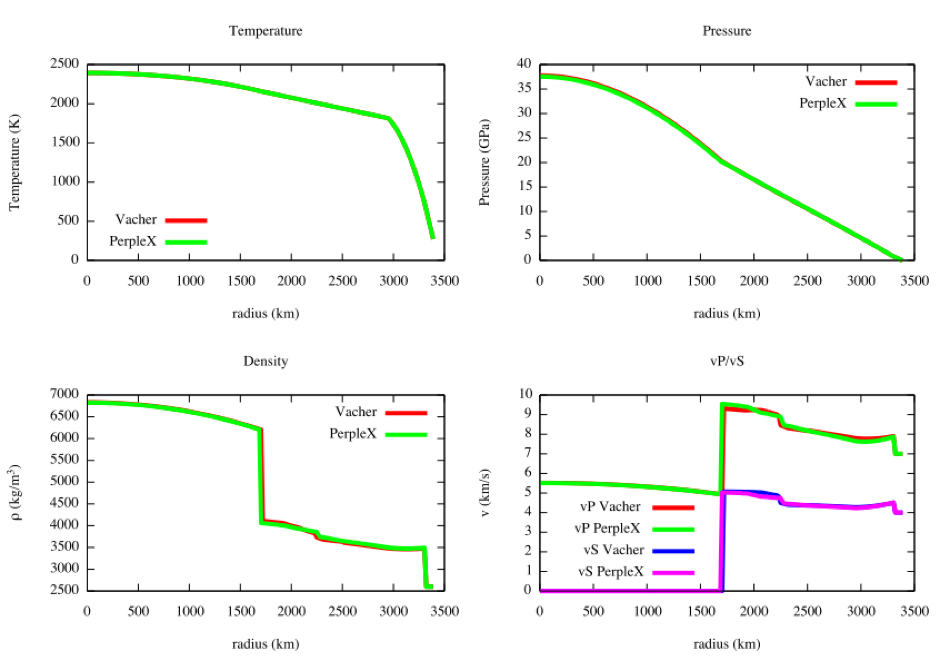
\includegraphics[width=0.85\textwidth]
{figures/FigDWTh.png}
\caption{Temperature, pressure, density and seismic velocities profiles in the Martian mantle for a Dreibus-W\"{a}nke composition \citep{Dreibus&Wanke1985} associated to the hot end-member temperature profile of \cite{Plesa2016} and computed with the two Geophysics Mineralogical codes (Vacher for \cite{Vacher1998} and Perple\_X for \cite{Connolly2005}).}
\label{fig:FigDWTh.png} 
\end{center}
\end{figure}

\begin{figure}[h!]
\begin{center}
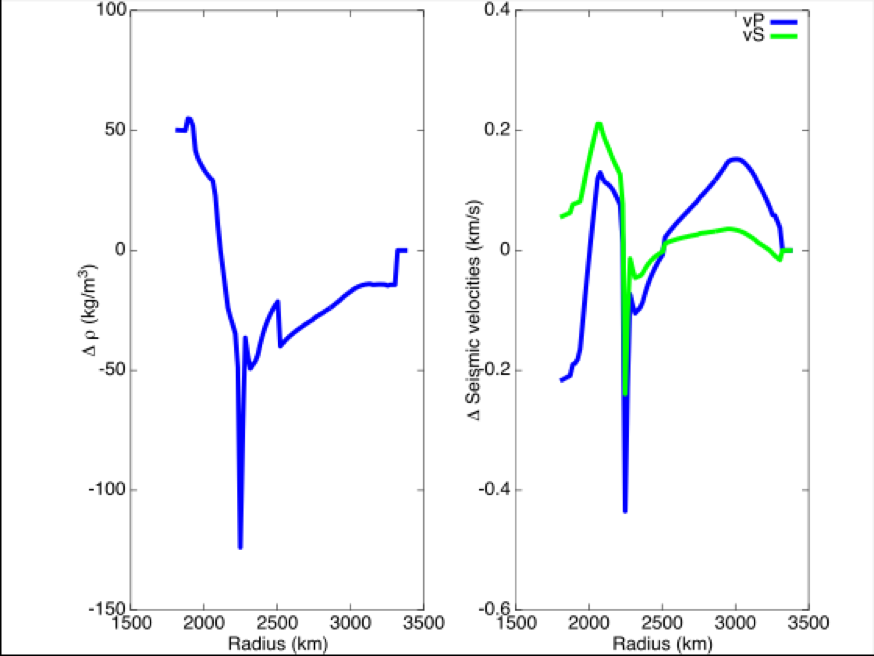
\includegraphics[width=0.65\textwidth]
{figures/FigDWThdiff.png}
\caption{Difference in density and seismic velocities values computed with the two Geophysics Mineralogical codes for a Dreibus-W\"{a}nke composition (Dreibus and W\"{a}nke, 1985) associated to the hot end-member temperature profile of Plesa et al (2016). The location of the phase transition at radius of approximately 2300 km differs by about 30 km between the two codes, leading to a large peak at that depth.}
\label{fig:FigDWThdiff.png} 
\end{center}
\end{figure}

\subsubsection{Discussion of the uncertainties of mineralogical modeling}
\label{discussionofuncertainties}
%\textcolor{orange}{(Rivoldini, Myhill, Verhoeven, Khan, Gudkova)
%thermodynamic equilibrium and introduction of oxygen and sulfur as independent components to the mantle.
%[30 lines. What is missing from the approach of the above section, estimations of the uncertainties. Maybe one Figure, but error bars will be added to the figures of 3.2.1.2 and of 3.3. Total 1 page]}

%In this subsection, we discuss the sources of uncertainty associated with forward modelling seismic velocities in Mars??? mantle. We will limit this discussion to uncertainties associated with modelling a homogeneous, texturally isotropic mantle in local thermodynamic equilibrium
While there are many possible sources of error associated with forward modeling of seismic velocities in Mars' mantle, we first consider here the uncertainties associated with modelling a homogeneous, texturally isotropic mantle in local thermodynamic equilibrium.
In the infinite-frequency limit and for a rock of a given composition at a given pressure and temperature, errors in modelled seismic velocities can arise from two sources: 1) inability of the equation of state, solution model and aggregate formulations to match real behaviour, and 2) incorrect thermodynamic and elastic parameter values for the endmember or solution models. 

For the majority of silicate and oxide minerals relevant to Mars' mantle, the quasiharmonic approximation of Stixrude and Lithgow-Bertelloni (2005; 2011) provides a reasonable estimate of elastic seismic velocities. Jacobs et al. (2017) show that thermodynamic models described using a single (volume-dependent) Einstein or Debye temperature can produce seismic wave velocities within 1\% of the measured velocities over a range of pressures and temperatures spanning much of Earth's upper mantle. 

The largest contributor to errors in seismic velocity calculations is probably uncertainty in laboratory measurements. Both the location of phase transitions and the seismic velocities of phases at high temperature and pressure can differ significantly between studies. For example, the pressure of the ringwoodite to bridgmanite + ferropericlase reaction varies by $\sim$2 GPa between different research groups (c.f. Ye et al., 2014). As another example, the aggregate $V_P$ and $V_S$ velocities of San Carlos olivine (fo90) derived from Brillouin spectroscopy can differ by as much as 2\% at high pressure (Zha et al., 1998; Mao et al., 2015), for reasons that are not yet clearly understood, but may be the result of nonhydrostatic stresses in the diamond anvil cell. Connolly and Khan (2016) recently made the first effort to quantify the seismic implications of experimental uncertainties. 

Aside from any updates and extensions to existing datasets, mineralogical mapping for the InSight Mission will be conducted with the thermodynamic dataset of Stixrude and Lithgow-Bertelloni (2011). This dataset contains minerals in the chemical system \ce{Na2O-CaO-FeO-MgO-Al$_2$O$_3$-SiO$_2$}. This system probably accounts for $>$97 wt\% of the bulk composition of Mars (Dreibus and W\"{a}nke, 1984), and therefore any additional components will have a small influence (probably <10 m/s) on seismic velocities. Nevertheless, it is worthwhile to consider the hosts for minor components in Mars' mantle. The most significant of these are probably MnO, Cr$_2$O$_3$ and S, which are all predicted to have abundances of $>$0.2 wt\% in Mars (Dreibus and W\"{a}nke, 1985; Tuff et al., 2013). At low oxygen fugacity, sulphur in Mars' mantle will be incorporated into iron sulfide. Manganese readily substitutes for magnesium or iron within olivine, pyroxene and garnet (Nishizawa et al., 1972; Balta et al., 2011), and is therefore unlikely to significantly affect phase proportions or stabilities in Mars' mantle. In contrast, chromium is preferentially incorporated into spinel at low pressures, stabilising it relative to other alumina-rich phases such as feldspar and garnet (Ziberna et al., 2013). Although chromium is not included in the Stixrude and Lithgow-Bertelloni dataset, it is included in the NCFMASCrO solution models of Jennings and Holland (2015). Using this dataset with the Dreibus and W\"{a}nke (1985) bulk composition, we investigate the effect of including Cr$_2$O$_3$ rather than replacing it with a mole-equivalent amount of Al$_2$O$_3$. Chromium expands the spinel stability field from a narrow wedge between the plagioclase and garnet-bearing fields restricted to $<$1000 K and $<$0.8 GPa to a field that extends up to the melting point at ~1.5 GPa. Bulk sound velocities increase by 0.2-1\% where spinel partially replaces plagioclase (at $<$1 GPa), and decrease by up to 1\% where spinel partially replaces garnet. The decrease in velocity due to adding chromium persists at higher pressure where spinel is not stable, but the perturbation is reduced to $\sim$0.25\%. This reduction is equivalent to a $\sim$50 K increase in temperature (for Vp $\approx$ 8 km/s and dVp/dT $\approx$ 0.4 m/s/K).

One additional independent component that is not included in the current modeling effort is oxygen. At low pressures, Mars is sufficiently reduced that iron is present almost exclusively as Fe$^{2+}$, either within silicate minerals or iron sulfide. At high pressures, however, iron undergoes an autoredox reaction, producing metallic iron and Fe$^{3+}$ (e.g. Frost and McCammon, 2004; Rohrbach et al., 2007). Although this reaction has not yet been documented in Mars-like compositions, it should take place regardless of the bulk composition. Near to the base of Mars' mantle, the main host for ferric iron is garnet, such that the key reaction will be

\ce{3Fe2SiO4} (ferroringwoodite) $\rightarrow$ \ce{Fe3Fe2Si3O12} (skiagitic garnet) + Fe (metallic iron/sulfide).

This reaction will reduce the amount of ringwoodite relative to calculations assuming all iron as Fe$^{2+}$. According to the model of Jennings and Holland (2015), skiagitic garnet has a bulk sound velocity 94\% that of ringwoodite at the P-T conditions of Mars' deep mantle. Ferric-ferrous iron ratios in majoritic garnets from laboratory experiments suggest that a skiagitic component may be the dominant iron-bearing endmember at $>$14 GPa (Rohrbach et al., 2007). The experiments of Bertka and Fei (1997) suggest that $\sim$40\% of Mars' lowermost mantle is garnet and that a skiagite component comprises $\sim$20\ mol \% of this garnet. In this case, one should expect a 0.5\% velocity reduction due to the autoredox reaction. Work is in progress to better understand the chemical and physical implications of these reactions on Mars' deep mantle.

\subsubsection{Pre-launch review of the geophysical parameters}
\label{sec:geophys}
%Review of the existing models for density, vp, vs, electrical conductivity, Qs, (Panning, Johnson, Khan, Giardini, van Driel, Staehler, Langlais, Gudkova, Mocquet, Dehant) [30 lines, May focus more on the historical evolution of the a priori models, from the mid 70th ( e.g. MARS AR, i.e. a PREM like model only corrected from pressure) to the modern a priori models and those defined as a priori model for InSight. Maybe add the Figure shown by V.Dehant on the Evolution of the core radius in the literature, with the most recent updates. Total 1 page]
\paragraph{Bulk structure constraints}
Prior to good constraints on Mars radius and oblateness from Mariners 4 and 9, the earliest estimates of Mars interior structure varied from estimates with a small dense core (Jeffreys, 1937) to a mostly undifferentiated body (Urey, 1952).  After the Mariner 4 flyby in 1965, and the Mariner 9 orbiter in 1971, improved estimates of the normalized polar moment of inertia (C/MR$^2$, where C is rotational moment of inertia, and M and R are the mass and radius of Mars) to $\sim$0.377, assuming hydrostatic equilibrium, allowed for improved models with either small Fe-Ni cores (Binder, 1969) or a range of larger core sizes with a mixture of Fe and FeS (Anderson, 1972; Johnston et al., 1974).  By the late 1970's, the estimate of the moment of inertia had been further revised to 0.3654 after taking into account isostatic compensation and the mass of Tharsis (Reasenberg, 1977), which is closer to refined estimates after the Pathfinder mission in the 1990's of 0.3662 (Folkner et al., 1997), although a broad range of values from 0.345 to 0.365 was still permitted by the data (e.g. Bills, 1990).  Improved models at this time matched this value and assumed simple layered models (crust, mantle with a phase transition corresponding to the olivine-spinel transition, and core), with linear gradients of elastic and density structure within these layers scaled from Earth models by the lower pressure gradient, e.g. model AR (Anderson et al., 1977; Okal and Anderson, 1978).  There have been many further refinements since this time, taking into account refined estimates of Martian chemical makeup and thermal structure, and improved mineral physics modeling to more accurately represent density, elastic and attenuation structure as discussed in more detail in section \ref{sec:geo_min_link} (Zharkov et al., 1991; Longhi et al., 1992; Kuskov and Panferov, 1993; Mocquet et al., 1996; Sohl and Spohn, 1997; Yoder and Standish, 1997. Bertka and Fei, 1998; Sanloup et al., 1999; Zharkov and Gudkova, 2000, 2005; Kavner et al., 2001; Yoder et al., 2003; Gudkova and Zharkov, 2004; Verhoeven et al., 2005; Sohl et al., 2005; Khan and Connolly, 2008; Zharkov et al., 2009; Rivoldini et al., 2011, Wang et al., 2013; Khan et al., 2017). 

\paragraph{Constraints on the core}
%(Weber, Rivoldini, Giardini, Garcia, Johnson, Dehant)
%[30 lines, focus on the a priori constraints for geophysical parameters (e.g. density, vp, vs if inner core, electrical conductivity, core ellipticity, etc., 2 Figures, Total 1 page]

After the moment of inertia number had finally been constrained after the Mars Pathfinder mission (Folkner et al., 1997), many new models were created using a variety of chemical models for Mars (e.g. Dreibus and W/"{a}nke, 1985; Morgan and Anders, 1979). Further progress can be associated with constraints on the tidal Love number k2 (Yoder et al., 2003), which showed Mars to have a liquid core. While the proposal of a liquid Martian core was made previously (e.g. Lognonne and Mosser, 1993; Zharkov and Gudkova, 1993, 1997), many earlier models had assumed a solid core due to the lack of a significant internal magnetic field.  Further model refinements were permitted by laboratory experiments on the compressibility and phase transformations of the predicted compositions of the Martian mantle using laboratory high-pressure facilities at high temperatures such as those performed by Kamaya et al. (1993) for the chemical model by Morgan and Anders (1979) and for the Dreibus and W\"{a}nke (1985) model by Bertka and Fei (1997, 1998).

Recent models of Mars are qualitatively similar, although modeling methods differ. The current best estimate of the radius of the Martian core ($\sim$1720-1810 km) (Khan et al., 2018) has increased substantially due to the increased value of k2 (Konopliv et al., 2006, 2011, 2016) in comparison with Yoder et al. (2003).  Overall, one of the biggest sources of uncertainty in a priori modeling of Martian structure remains the tradeoff between core density and size (figure \ref{fig:Figsulfur.png}).

\begin{figure}[h!]
\begin{center}
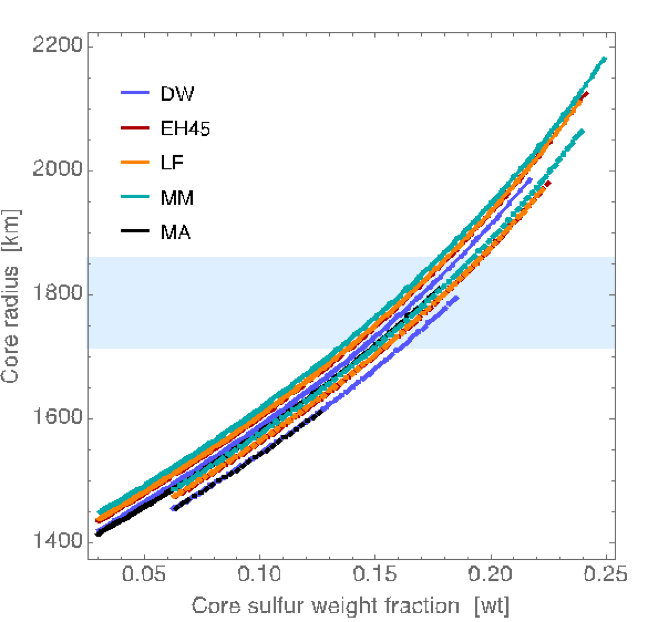
\includegraphics[width=0.65\textwidth]
{figures/Figsulfur.png}
\caption{Core radius as a function core sulfur concentration for the hot (solid curves) and cold (dashed curves) mantle temperature profile.  The blue shaded area represents the core radius range in agreement with the k2 value of Konopliv et al. 2016 and Genova et al. 2016. The acronyms stand for the different mantle mineralogy models (DW: Taylor [2013], EH45: Sanloup et al. [1999], LF: Lodders [2000], MM: Mohapatra and Murty [2003], MA: Morgan and Anders [1979]. Models agree at 1-sigma with the average moment of inertia of Mars (MOI=0.3639$\pm$0.0001) [Konopliv et al., 2016].}
\label{fig:Figsulfur.png} 
\end{center}
\end{figure}
All these models provide relatively large core rich in sulfur, implying that an inner core is quite unlikely today.

%\textcolor{purple}{Notes from Tilio:
%I am not aware of any publication showing vs profiles for the inner core. I have addressed the question of the presence of an inner core in dpi: 10.1016/j.icarus.2011.03.024.
%But in that publication I did not show the vs profiles in the inner core. Needless to say, the large core of Mars requires quite a lot of sulfur implying that an inner core is quite unlikely today.
%Moreover, because of the large amount of S, solid Fe crystallization if the core temperature would allow for it, would result in snow formation, possibly leading to top-down inner core formation if 
%the composition in sulfur is below the eutectic composition and to the formation of Fe-S compounds if the composition of the core is larger than the eutectic composition. Those compounds might sink or float up. But his has not been studied in detail yet. A discussion of this can be found here doi: 10.1186/s40645-017-0139-4. As you can see from that publication, for crystallization to happen at all a very low temperature is required, not at all in agreement with thermal evolution models. If required I can produce figures that show velocities in the core and inner core, but the core radii of those models are small and not in agreement with observed tides.}

\paragraph{Constraints on seismic attenuation}
The first discussion on seismic attenuation in the Martian interior was by Lognonn\'{e} and Mosser (1993) where the authors converted the shear attenuation, Q$_{\mu}$, distribution of the Earth model PREM (Dziewonski and Anderson, 1981) to the conditions of Mars, accounting for temperature differences and integrated from the Q estimated from the Phobos tide secular acceleration. More detailed investigation of anelasticity of the Martian interior and estimates of the dissipative factor were then considered in Zharkov and Gudkova (1997) and more recently by Zharkov et al. (2017). All these first studies were based on the extrapolation of an Anderson and Given (1982) attenuation model to Mars conditions, in which seismic Q is defined as a power law function of frequency with an exponent $\alpha=0.15$ in a seismic bandwidth between corner frequencies $f_1$ and $f_2$ and a steeper exponent of 1 or -1 below or above the bandwidth, respectively. More recently, Khan et al (2016, 2017) proposed to use a consistent model for the frequency dependency of both Q and seismic velocities based on a Burger derived model from the work of Jackson and Faul (2010). This model, however, essentially also predicts effectively a power law for Q (e.g. Bellis and Holtzman, 2014) with a larger exponent $\alpha \approx$ 0.2--0.3 in the seismic bandwidth, but a less steep slope ($1-\alpha$) for frequencies below the seismic band.  Although many experimental data support a relatively constant power law at frequencies less than 0.1 Hz and therefore a Q increase towards high frequencies, experimental data (e.g. Jackson and Faul, 2010, Fontaine et al., 2015) shows that such a constant power above 0.1Hz is not a robust assumption, as the Q might converge towards a plateau around 1 Hz and even decrease at higher frequencies.  In addition, large discrepancies are already found between Earth observations and laboratory data, as summarized by Lekic et al. (2009) and Romanowicz and Mitchell (2007, 2015). Understanding the frequency dependence of Q is essential in order to relate attenuation within the seismic band to constraints at the Phobos tidal period.  Using different estimated exponential slopes for the Q frequency dependence from the estimated Phobos Q (85 $\pm$ 5), which is mostly controlled by average Q$_{\mu}$ in Mars' mantle at tidal frequencies, could lead to Q increase by a factor of 2.1, 3.1 and 4.6 at 10 sec respectively for $\alpha$=0.1, 0.15, 0.2, and therefore to larger Q at 1 Hz. Proposed values range therefore from less than about 200 for Zharkov and Gudkova (2017) and Khan et al. (2018) who use $\alpha\leq 0.1$ to 250-300 for Lognonn\'{e} and Mosser (1993) and Zharkov and Gudkova (1997), who used 0.15.

%Nevertheless and to first order, the Phobos Q = 85 ? 5, as mostly related to the average shear Q in the Mars Mantle, could lead to Q increase by a factor of 2.1, 3.1 and 4.6 at 10 sec respectively for a=0.1, 0.15, 0.2, and therefore to large Q at 1 Hz (ranging from 250 to 300 for Lognonn? & Mosser, 1993, Zharkov and Gudkova, 1997 who used 0.15 but less and about 200 for ?and Zharkov and Gudkova, 2017).

Another approach to estimating seismic Q on Mars rather than the use of the Phobos tide Q might be based on scaling from Earth observations. This is based on the assumption that Q is given by (e.g. Jackson et al., 2002)
\begin{equation}
Q^{-1}=A\left[ { 1 \over f d}\exp\left(-{E+pV \over RT}\right)\right]^{\alpha},
\end{equation}
where $A$ is a constant, $a$ the power law slope, $f$ and $d$ the frequency and grain size, $E$ and $T$ the activation energy and thermodynamical temperature, while $p$ and $R$ are the pressure and ideal gas constant, and $V$ is the activation volume. By taking (2) for a given frequency, pressure and size grain but two different temperatures T and T$_0$, we then get :
%\textcolor{red}{Mark: Please check this equation, which was written as Q-1=A[f-1d-1exp(-E+pVRT)] in the original Word file by Philippe, which was hard to read and appeared to have the wrong frequency dependence. I've attempted to correct it, but I may have introduced new errors.  I also added a $b$ term to the equation below, which was missing from the original Word file but referenced in the following text, and changed it to a $\Delta T$ rather than T, which makes more sense, unless you define $Q_0$ at 0K.  I also called $V$ the activation volume... is this what you meant?} This leads to a temperature dependency of Q which can be written as
\begin{equation}
Q^{-1}(T) = Q_0^{-1}\exp\left(-b \ ({1 \over T} - {1 \over T_0})\right) ,
\end{equation}
where $Q_0$ is the observed quality coefficient at a reference temperature $T_0$ and Q the predicted one at T. Here, $b=\alpha \ {E+pV \over RT}$.
% originally written as Q-1 = Q0-1exp(-T), which didn't exactly make sense
 Large variations remains however in estimation of the $b$ parameter, which range from $\sim$13500 K for Jackson et al (2002) (for E=424kJ/mole, $\alpha$=0.26, p=0) to 3540 K for Fontaine et al. (2005). We use the value of Lognonn\'{e} \& Mosser (1993) of 4530 K as a mid range example (with E=251kJ/mole, $\alpha$=0.15), and extrapolate from the reference Q of 173 for the Earth's upper mantle (outside the Earth Low Velocity zone) based on the PREM model (Dziewonski and Anderson, 1981). This is shown for the difference a priori reference Mars models and associated temperature structures in Figure \ref{fig:FigshearQ.png}. For depth less than 300 km, all Mars models suggest a mantle colder than Earth at the same pressure, and likely larger Q. But deeper than 300 km, the Earth mantle could in contrast be colder than Mars for the same pressure, and temperature effects will reduce Q.

\begin{figure}[h!]
\begin{center}
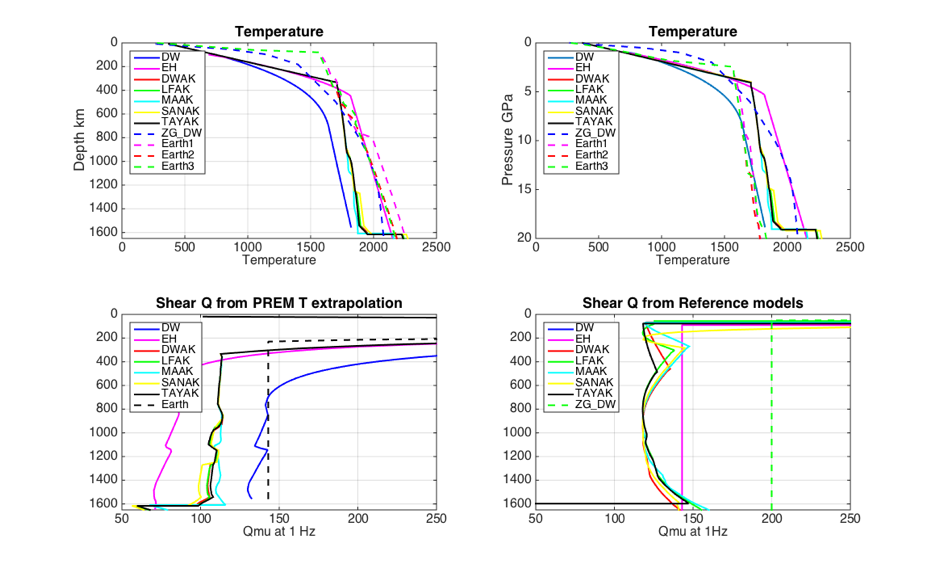
\includegraphics[width=1.1\textwidth]
{figures/FigshearQ.png}
\caption{On the top, Reference models temperature as function of depth (on the left) and Pressure (on the right) as compared to Earth Temperature models. See section 3.3 for more details on these reference models. On the bottom, comparison between on left, the shear Q as extrapolated from PREM with relation (3) and on right, the shear Q proposed for these reference models.The acronyms correspond to models listed in Table 4 or stand for the different mantle mineralogy models (DW: Taylor [2013], EH45: Sanloup et al. [1999], LF: Lodders [2000], MM: Mohapatra and Murty [2003], MA: Morgan and Anders [1979]).}
\label{fig:FigshearQ.png} 
\end{center}
\end{figure}

\subsection{Examples of multiparameter approaches and InSight payload complementarity}

As Insight will deploy a wide set of geophysical instruments, constraints will be made on the seismic velocities v$_p$ and v$_s$ by propagating waves recorded by SEIS, on the impact of density profile on the rotation as recorded by RISE and on the electrical conductivity, as recorded by the IFG magnetometer. This will allow multiparameter approches and is illustrated by a few example below.

\subsubsection{RISE/SEIS:  CMB density jump and Body waves reflection}


The density jump at the CMB (Core-Mantle Boundary) can be constrained by two different approaches: the FCN (Free Core Nutation) period to be determined by RISE and the reflection coefficients of seismic core phases from SEIS. In order to illustrate the dependence of these two observables on the CMB density jump, these parameters were estimated for a wide range of interior structure models, including the 14 a priori Mars models used in a recent blind test experiment for marsquake location (Clinton et al., 2017).

The FCN period is a good indicator of the density jump as illustrated in Fig \ref{fig:figabc}a (see also Van Hoolst et al. 2000). It increases almost linearly with decreasing density jump at the CMB with limited spread due to different mantle mineralogy, core composition and thermal state. As observed in figure \ref{fig:figabc}b, for epicentral distance smaller than 90$^{\circ}$, the seismic body wave reflection coefficients are significant only for ScSH, ScSV, ScP and PcP. The variability in these coefficients between various models is mainly controlled by the impedance ratio at CMB. A difficulty in the analysis of body wave amplitudes is the influence of source radiation on these parameters. In order to remove this influence, we suggest the use of ScP over ScSV amplitude ratios. These two phases experience approximately the same radiation at the source. As observed on figure \ref{fig:figabc}c, this ratio is dependent on the density jump at CMB, in particular for epicentral distances larger than 50$^{\circ}$.
Since the two methods are fully independent, combining the FCN frequency and body wave amplitude ratios can strongly constrain the CMB density jump.

\begin{figure}[hp!]
\begin{center}
\subfloat[]{
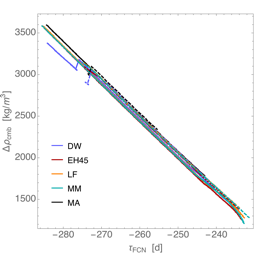
\includegraphics[width=0.50\textwidth]{figures/figa.png}
\label{fig:figa.png}}

\subfloat[]{
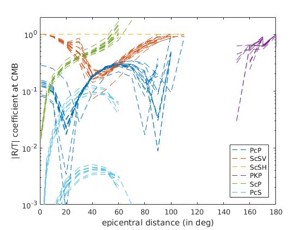
\includegraphics[width=0.50\textwidth]
{figures/figb.png}
\label{fig:figb.png}}

\subfloat[]{
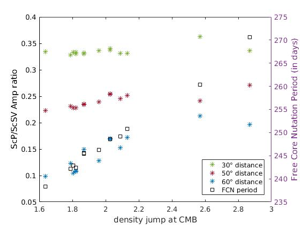
\includegraphics[width=0.50\textwidth]
{figures/figc.png}
\label{fig:figc.png}}
\caption{{a) Relation between density jump at the core-mantle boundary and FCN period for the hot (solid curves) and cold (dashed curves) mantle temperature profile. See Figure 14 and table 4 for legend explanation.
b) Reflexion/transmission coefficients at CMB for various core phases (color code) as a function of epicentral distance (in degrees). The various lines represent the estimates for the 14 a priori models.
c) ScP/ScSV amplitude ratio (stars) and FCN period (in days, open squares) as a function of the relative density jump at the CMB (varying with a priori model). Amplitude ratios are given for 3 different epicentral distance range (color code).}}
\label{fig:figabc}
\end{center}
\end{figure}

\subsubsection{Orbiters/SEIS: Sun k$_2$-ScS travel times}
As noted in Section 2.5, geodesy provides the best constraints on the core size and among those, the Love number k$_2$ is the most sensitive one. For a planet with a liquid core, the elastic deformation of the tide is distributed between the two free surfaces located at the planetary surface on one side and at the Core Mantle Boundary on the other side. A fundamental bias is however found between the shear modulus and the thickness of the mantle, and models with smaller shear modulus but larger mantle will lead to similar k$_2$. See Lognonn\'e \& Johnson (2011, 2015) for an example of this non-unicity of the k$_2$ constraints for the Moon. The 4.9\% error in the $k_2$ determination leave therefore a wide range of freedom in the core size.\\
For ScS travel times, the bias between S waves velocities and mantle depth is the opposite and smaller velocities request smaller depth for a given travel time. The joint inversion of both k$_2$ and ScS travel time will therefore improve greatly the determination of both the mantle structure and depth of the CMB.
Figure \ref{fig:FigureScS.png} shows the differences in core size of the Reference models, detailed in section 3.3 and listed in Table \ref{table:TableModel}. The core radius varies from 1520 km for model SAAK up to 1850 km for model EH45TC. SAAK model, which is has a marked shear waves low velocity zone in the mantle, illustrates well the bias between core depth and mantle shear wave velocity discussed above. If we do not consider such low velocity zone, all models without strong low velocity zone range therefore from 1685km to 1850 km, $\pm$ 82.5 km around the median core radius. As discussed above and already shown by Panning et al. (2017), the core reflected travel time of ScS will provide key new and robust constraints on the core size as illustrated on Earth and more recently on the Moon by Weber et al. (2011) and Garcia et al. (2011). This is also demonstrated by the 150 sec of travel times differences between the two extreme ScS travel times. These two data will therefore be crucial in determining the deep Mars structure and, together with RISE constraints, providing the core radius.
\begin{figure}[h!]
\begin{center}
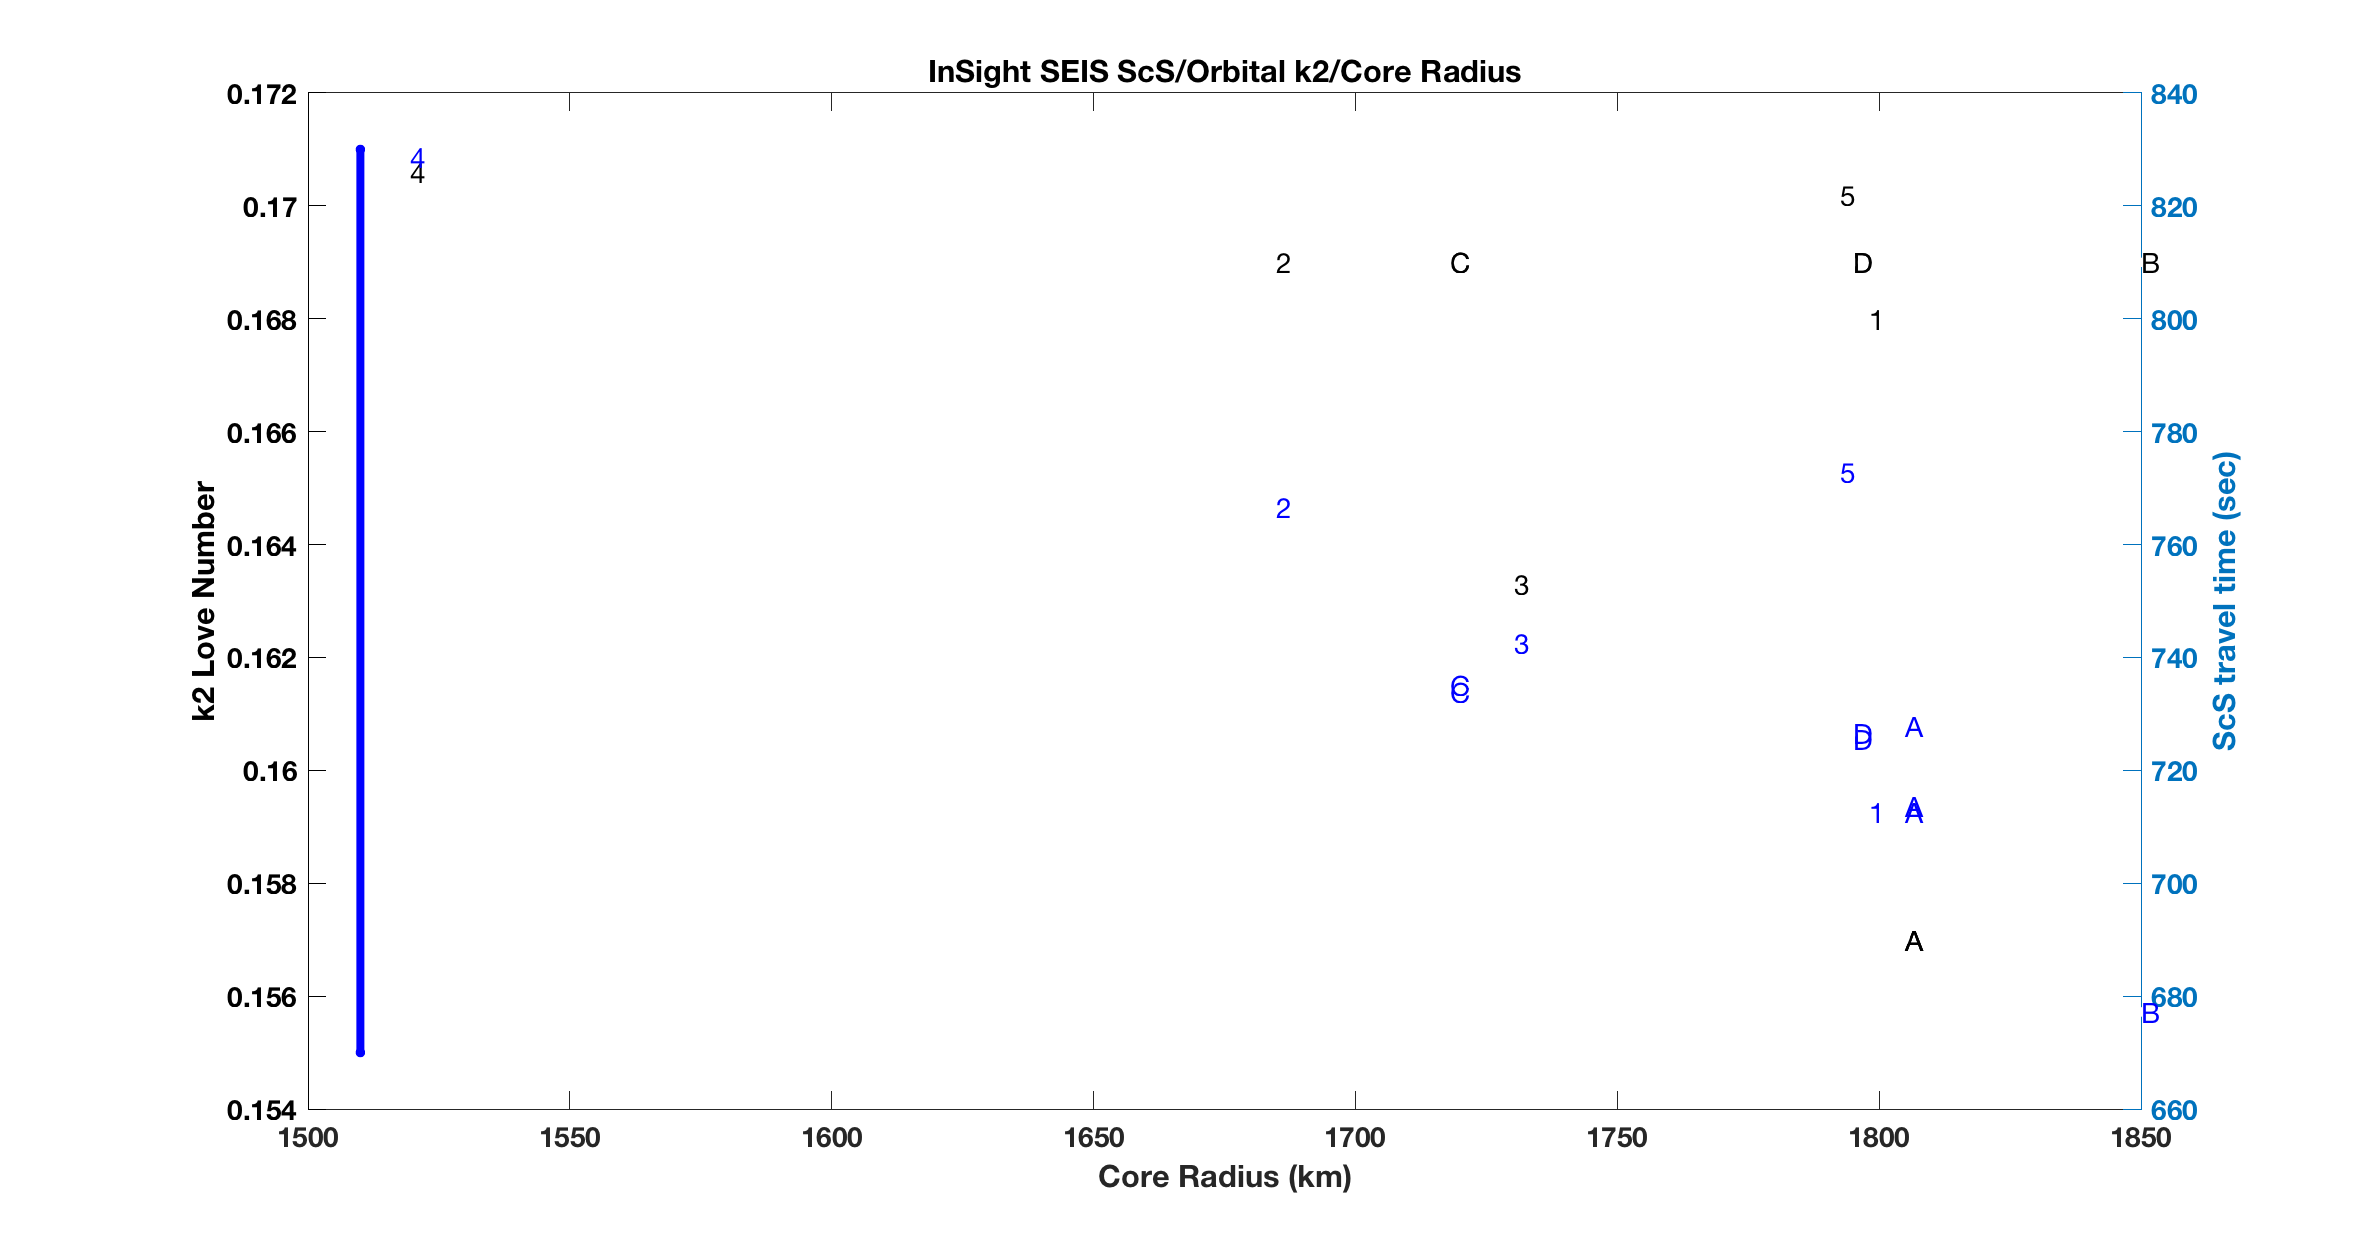
\includegraphics[width=1\textwidth]
{figures/FigureScS.png}
\caption{Values of the Love number k$_2$ (in black on the left) and of the ScS travel time (in blue on the right) for all Reference models described in section 3.3. See Table \ref{table:TableModel} for all values as well as model Letter.}
\label{fig:FigureScS.png} 
\end{center}
\end{figure}

\subsubsection{SEIS/IFG: Vs-Qs and electrical conductivity measurements}

Another important geophysical parameter which can be estimated in advance of the arrival of InSight is the electrical conductivity of the Martian mantle, which represents a signature of the interior which is complementary to seismic velocity (Khan et al., 2006a,b). Such complementarity of magnetic sounding and seismic studies has been demonstrated using Martian synthetic data \citep{Mocquet&Menvielle2000, Verhoeven2005}. The mantle of Mars is characterized by a high iron content \citep{McSween1994}. This result in an order of magnitude increase in the electrical conductivity profile compared to that for the Earth's mantle \citep{Vacher&Verhoeven2007}.

Laboratory measurements of the electrical conductivity of hydrogen-iron bearing mantle silicate minerals have shown that different conduction mechanisms, involving different charge carriers, occur at pressure and temperature conditions relevant to planetary mantles \citep[see e.g. the reviews of][]{Yoshino2010, Karato2011}. In a recent paper, \cite{Verhoeven&Vacher2016} have shown that the small polaron conduction, associated with charge transfer between ferrous and ferric ions, dominates the conductivity at iron and water contents relevant to the Martian mantle.

Figure \ref{fig:conduct.png} shows the electrical conductivity profiles computed using the modeling of \cite{Verhoeven&Vacher2016} for compositions and temperature profiles of the Martian mantle associated with the MSS models of \cite{Panning2016}. The electrical conductivity for the laboratory-based composition model of \cite{Bertka1997}, along with the data-based profile derived by \cite{Civet&Tarits2014} from MGS magnetic field measurements are shown for comparison. In the first thousand km depth, different composition models for the same temperature profile have almost the same electrical conductivity. In contrast, there is a difference of almost one order of magnitude between the electrical conductivity for the cold and hot temperature profiles for a given composition. This suggests that the electrical conductivity can be considered as a good proxy of the mantle temperature in this depth range. This conclusion does not hold below 1000 km depth, where high pressure phases lead to an increasing dependence of electrical conductivity on composition effect. Note that the \cite{Civet&Tarits2014} profile is characterized by 180 km layer thickness which induces some uncertainty in the location of the olivine transition around 1000 km depth.


\begin{figure}[h!]
\begin{center}
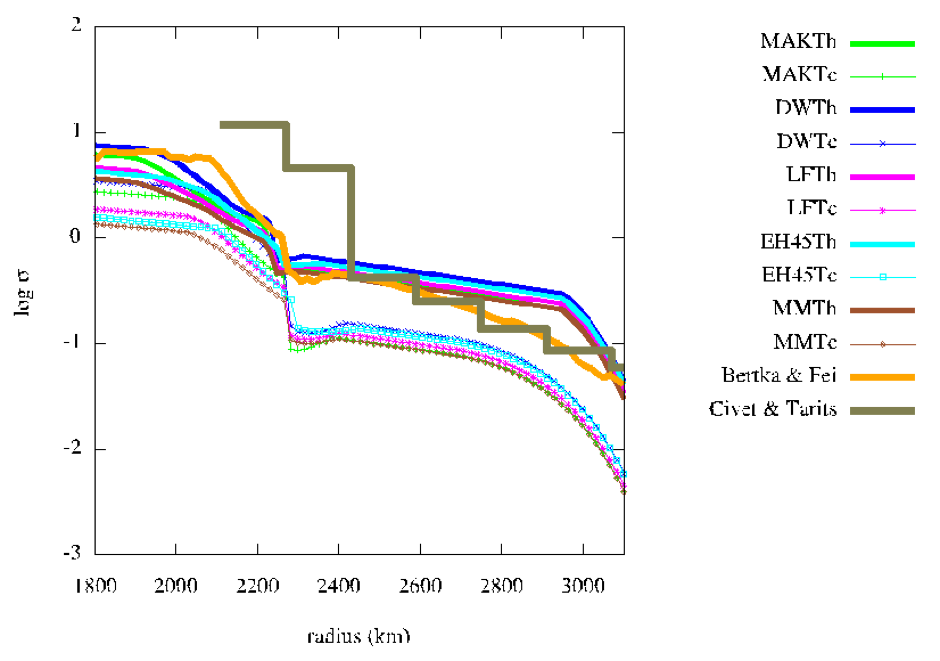
\includegraphics[width=0.75\textwidth]
{figures/Figconduct.png}
\caption{Electrical conductivity profiles corresponding to the composition and temperature profiles associated to the MSS models of Panning et al. (2017) and computed using the modeling of Verhoeven and Vacher (2016). MAK, DW, LF, EH45, MM represent the composition models of Morgan and Anders (1979), Dreibus and W\"{a}nke (1985), Lodders and Fegley (1997), Sanloup et al. (1999) and Mohapatra and Murty (2003), respectively whereas Th and Tc represent end- members temperature profiles from Plesa et al. (2016). The reference models of Bertka and Fei (1997) and Civet and Tarits (2014) are shown for comparison.}
\label{fig:conduct.png} 
\end{center}
\end{figure} 

\subsubsection{Velocity/density jump at the Moho}
Since the Martian surface is characterized by dipole topography, Mohorovicic discontinuity distribution will principally follow the topography anomaly in the opposite-sign manner due to the process of isostatic compensation. A combination of the topography measurement provided by Mars Orbiter Laser Altimeter (MOLA) and the Bouger anomalies estimated from MGS has enabled us to construct the models of Moho depth distributions (e.g. Neumann et al. 2004). The mean crustal thickness is believed to be 50-100 km with 600 kg/m$^3$ of density contrast. However, the ill-posedness of linear inversions hinders an unambiguous determination of crust-mantle density contrast and Mohorovicic depth. Chujkova et al. (2014) proposed to take into account the contribution of the quadratic terms of topographic masses and density contrast in the external gravity potential in order to tackle the problem, showing the feasibility in Earth’s case, but the spherical harmonic degree considered is very low (18). Furthermore, Mohorovicic estimation using potential data is hampered by a strong non-equilibrium due to the dichotomy (e.g. Gudkova et al. 2017) and the sharpness and lateral distribution of density around Moho discontinuity are really hard to look at. It is thus important to give a seismic constraint on seismic velocity and density jump and their depths from SEIS measurement. Since the velocity-density empirical relationship (e.g. Barton 1986) could sometimes encounter disagreements even in some places in Earth (e.g. Hsieh \& Yen 2016), it will be interesting to first investigate velocity by teleseismic refraction data independently from potential data, so that we be able to infer rock types.

Yet, seismological observations from refraction data might not be sufficient to constrain the Mohorovicic discontinuity due to its smoothed feature. In order to exploit the information on the structural effects beneath the seismic station embedded especially in high-frequency contents of SEIS teleseismic events, we will calculate receiver functions by removing the source-time function effects as well as the far deep mantle structure (e.g. Vinnik 1977; Kumar et al. 2010) and we will be also able to perform multi-parameter inversion using the receiver function (e.g. Bodin et al. 2014). Fig. 18 shows receiver functions for several given models with various epicentral distances.

\begin{figure}[h!]
\begin{center}
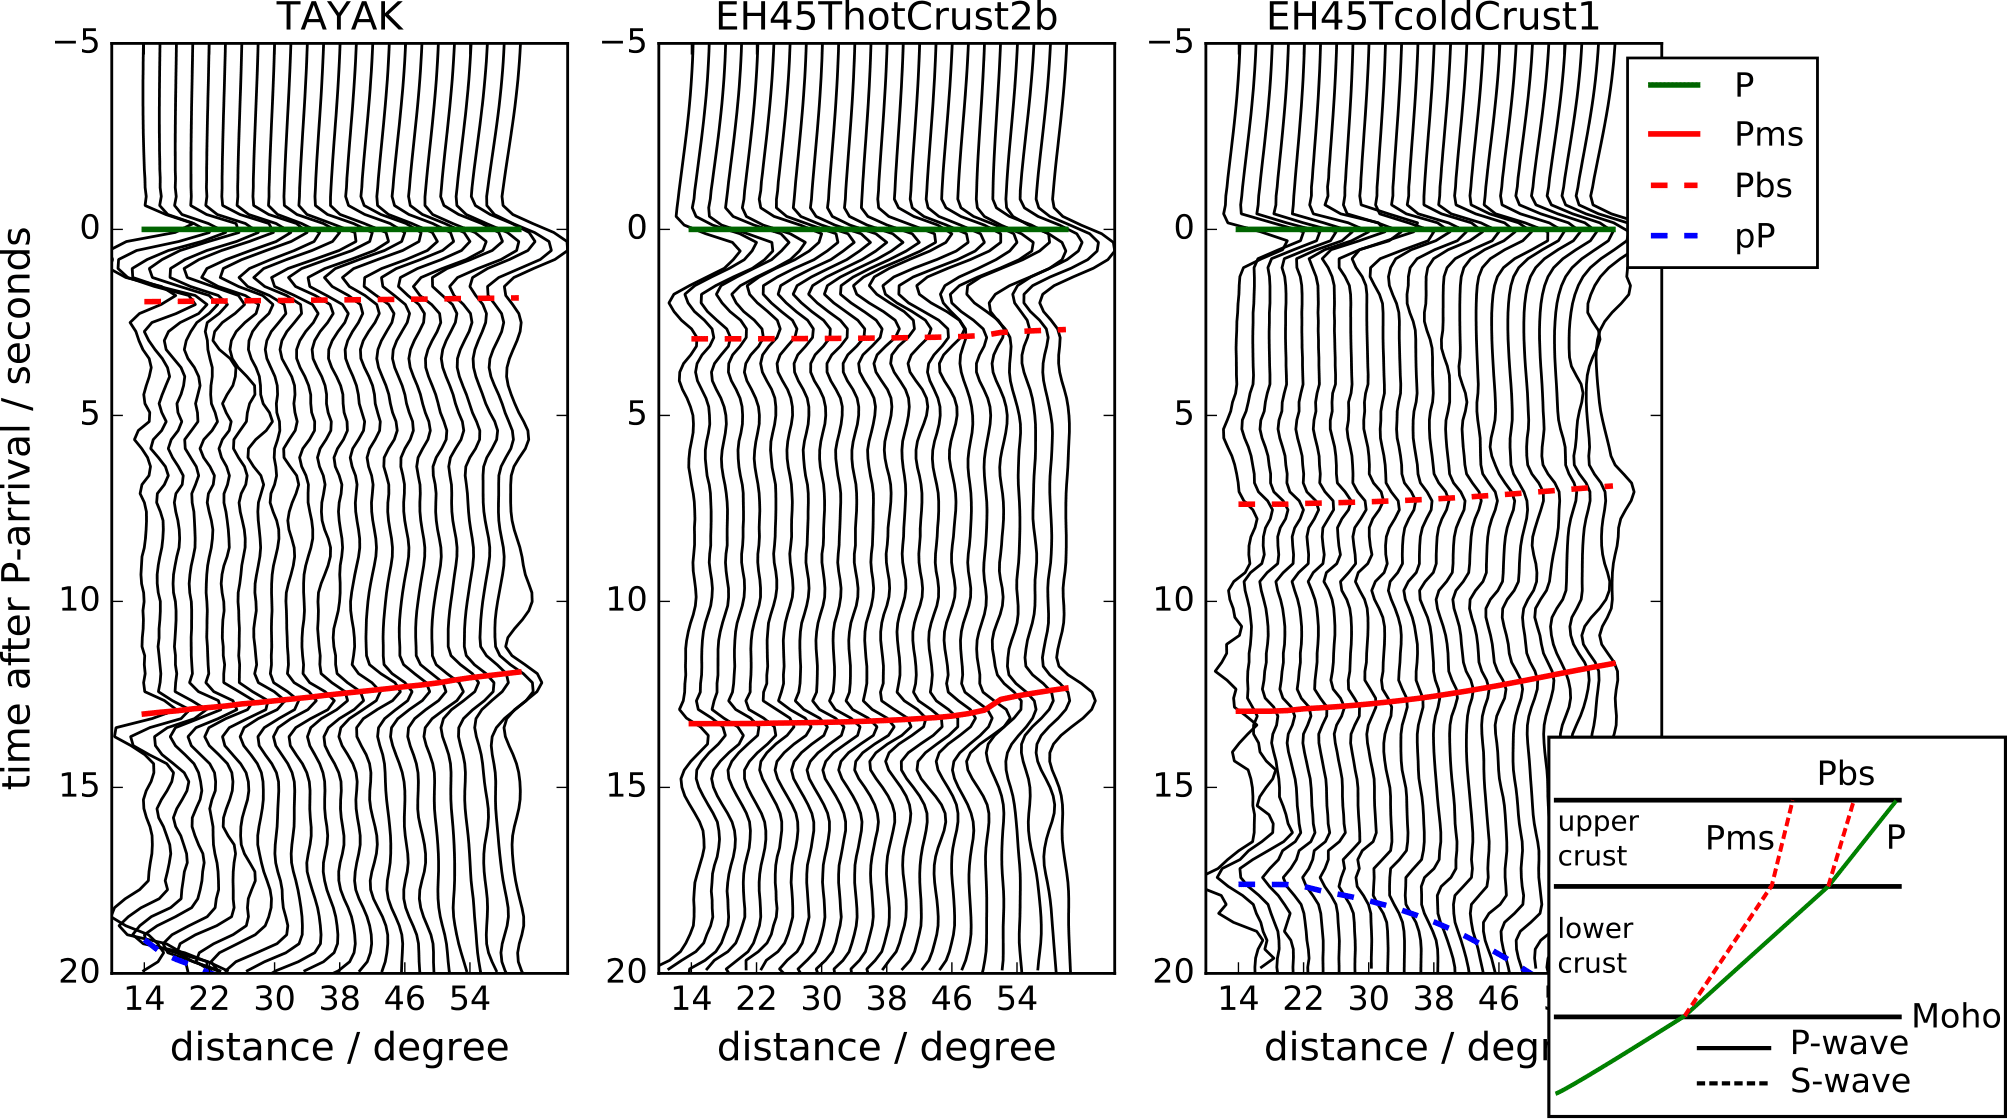
\includegraphics[width=1.0\textwidth]
{figures/Fig_waveforms.png}
\caption{Receiver function example for three models of the InSight Blindtestmodel suite \citep{Clinton2017}. The waveforms show the R-component of the P-wave coda of a 60 km deep event in various distances. Highlighted are the theoretical arrival times of P-S conversions at the Moho (Pms) or a mid-crust-discontinuity (Pbs). The converted waveforms are relatively low in amplitude, but especially Pms is clearly visible. The waveforms were calculated using AxiSEM and Instaseis \citep{Nissen-Meyer2014, VanDriel2015}}
\label{fig:waveform.png} 
\end{center}
\end{figure} 


Another factor to be considered is the existence/absence of an upper mantle low velocity zone due to a thick stagnant lid or local dissipation in the Martian mantle (Zheng et al. 2015), that can provoke a shadow zone for direct P- and S-waves. It will result in difficulty of receiver function analysis described above, although long-wavelength 1D imaging will not really affected by its existence or absence (e.g. Khan et al. 2016).



\newpage
\subsection{Reference Models \label{sec:models}}\subsubsection{1D Reference models}

As discussed in section~\ref{sec:geophys}, there is an extensive history of development of reference models for the Martian interior constrained by geodesy data and a range of geochemical and thermal models.  For the InSight mission, we have selected a range of reasonable models to serve as a representative range of models (figure~\ref{fig:Fig3_1_1.png} and table~\ref{table:TableModel}), similar to the range of models used for the recent blind test of Marsquake location methods (Clinton et al., 2017), modified to include models from Khan et al. (2017). The range is not meant to be an exhaustive distribution of all possible models, but rather to serve as a representative range of current modeling assumptions.  Eight of the models in the set (those with model names beginning with DWT or EH45T) are based on Rivoldini et al. (2011), and described in Panning et al. (2017).  The models beginning with DW are based on the bulk mantle composition defined by Dreibus and W\"{a}nke (1985), while those beginning with EH45 represent a bulk mantle composition created by a mixture of 45\% enstatite (EH) and 55\% ordinary (H) chondrites (Sanloup et al., 1999), using either hot or cold temperature profiles (Plesa et al., 2016), and a range of simplified crustal models.  The model labeled ZG\_DW is model M14\_3 of Zharkov et al. (2009), based on the Dreibus and W\"{a}nke (1985) chemical model. The top crustal layer is an averaged transition from regolith to consolidated rocks. The profiles of density and seismic velocities in the lower crust correspond to the mineralogical models constructed by numerical thermodynamical modeling (Babeiko and Zharkov, 2000), while the mantle model relies on the experimental data obtained by Bertka and Fei (1997). The core consists of iron-nickel with admixture of sulfur and hydrogen (Zharkov, 1996). The ZG\_DW model has been corrected for the larger k2 value in Zharkov et al. (2017).  The family of ``AK'' models are constructed assuming 4 different bulk mantle compositions (the preface to ``AK'' with DW, LF,  SAN, and TAY referring to Dreibus and W\"{a}nke (1985), Lodders and Fegley (1997), Sanloup et al. (1999), and Taylor (2013), respectively) and therefore mineralogy. These compositions derive from geochemical, cosmochemical, and isotopic analyses of Martian rocks and primitive solar-system material (e.g., Taylor, 2013). Based on these compositions, radial profiles of physical properties were computed using Gibbs free-energy minimization (for details the reader is referred to Khan et al. (2017)).  All models show a similar mantle velocity gradient, but show differences in the presence or absence of a low velocity zone in the upper mantle as well as the precise depth of phase transformations between 1000 and 1200 km depth.  Clear tradeoffs between core radius and density are also shown.

The shear attenuation models can be grouped into two categories: those models (``DW-,'' ``EH-,'' and ``ZG-'') that are scaled from the layers of the preliminary reference Earth model (PREM, Dziewonski and Anderson, 1981) or computed based on a specific viscoelastic model (extended Burgers rheology) (``AK-''). The latter models are temperature-, pressure-, and composition-dependent and vary continuously with depth, but generally produce lower Q estimates (higher seismic attenuation) within the mantle. Bulk attenuation is fixed to PREM and is relatively small (high Q) compared with shear attenuation. 

Major model properties are summarized in table~\ref{table:TableModel}. All models contain relatively large cores ($\sim$1700--1800 km in radius), in line with the inversion results of Khan et al. (2018) that indicate that only models with large cores are capable of fitting the currently available geophysical data (mean mass and moment of inertia and tidal response).

\begin{figure}[h!]
\begin{center}
\includegraphics[width=1.0\textwidth]
%\begin{enumerate}
%\item 
%\end{enumerate}
{figures/Fig3_1_1.png}
\caption{The set of 1D reference models defined as the reference set.  Panel A shows P velocity (solid line), S velocity (dashed line), and density (dotted line) for the set of reference 1D models with line color defined as in the legend in panel B. Panel B shows shear quality factor, while panel C zooms in on the mantle structure.}
\label{fig:Fig3_1_1.png} 
\end{center}
\end{figure}

\begin{table}
\centering
\caption{Summary of the models with respect to core radius, mean density, Normalized mean moment of Inertia, Sun Phobos and Secular attenuation of Phobos. The frequency attenuation power is also provided for link between the Sun and the Phobos tides frequencies, as well as the travel time of core reflected S waves. Models DWTH and EH45 have the k$_2$ values at Sun frequency and high (elastic) frequencies and have no further frequency dependency of elastic and anelastic  parameters.}
\label{table:TableModel}
\resizebox{\textwidth}{!}{
\begin{tabular}{|c|c|c|c|c|c|c|c|c|}
\hline
Model     & Letter  & Core radius & Mean density  & ${I \over Ma^2}$ & k$_2$ Sun & Q$_{Phobos}$ & $\alpha$ & ScS \\
Units     & & km          & kg/m$^3$      & none             & none      &  none         & none      & sec \\
\hline
DWTH      & A & 1805.0         & 3934.09      & 0.36398          & 0.170/1.57& 85           & N/A      & 727.8 \\
DWTHC1    & A & 1805.0         & 3934.09      & 0.36398          & 0.170/1.57& 85           & N/A      & 712.6 \\
DWTHC1b   & A & 1805.0         & 3934.09      & 0.36398          & 0.170/1.57& 85           & N/A      & 713.7 \\
EH45TC    & B & 1850.0         & 3934.09      & 0.36405          & 0.182/1.69& 93           & N/A      & 677.2 \\
EH45TCC1  & C & 1718.0         & 3934.09      & 0.36405          & 0.182/1.69& 93           & N/A      & 733.9 \\
EH45TCC1b & C & 1718.0         & 3934.09      & 0.36405          & 0.182/1.69& 93           & N/A      & 735.1 \\
EH45THC2  & D & 1795.0         & 3934.09      & 0.36405          & 0.182/1.69& 93           & N/A      & 725.6 \\
EH45THC2b & D & 1795.0         & 3934.09      & 0.36405          & 0.182/1.69& 93           & N/A      & 726.7 \\
ZGDW      & a & 1798.1         & 3935         & 0.3638           & 0.168     & 96.2         & 0.1      & 712.7 \\
DWAK      & b & 1780.1         & 3935.1       & 0.3638           & 0.169     & 88.1         & 0.26     & 766.7 \\
LFAK      & c & 1745.5         & 3935.1       & 0.3637           & 0.1633    & 95.5         & 0.31     & 742.5 \\
SAAK      & d & 1762.2         & 3934.7       & 0.3638           & 0.1706    & 89.6         & 0.29     & 828.7 \\
TAAK      & e & 1791.4         & 3934.7       & 0.3637           & 0.1702    & 109.7        & 0.34     & 772.8 \\
\hline
\end{tabular}
}
\end{table}

\subsubsection{1D Reference model sensitivities} \label{1D_ref_sensitiviies}

The elastic properties of planet forming materials are particularly sensitive to temperature variations and chemical composition. In the case of Mars, the FeO enrichment of the mantle and its possible content in volatiles, primarily \ce{H2O}, are particularly interesting to be considered, for they are intimately related to the accretion history of the planet and to its degassing and evolution. Temperature and chemical variations are mutually dependent and combine their effects on density and seismic velocity values. An example is the well-known phase diagram of the forsterite-fayalite \ce{[Mg_xFe_{(1-x)}]2SiO4} system, where the Clapeyron slopes of the exothermic olivine - wadsleyite - ringwoodite transitions and their locations at depth, depend both on temperature and on the Mg\# (Katsura and Ito, 1989). This dependence is particularly important inside Mars' mantle, where the iron content is suspected to be about twice the Earth's (see Section 2.2 above), and where the low gradient of pressure implies that a change of 1 GPa corresponds to a variation of about 85 km at depth (Mocquet et al., 1996). It also affects the non-olivine components of the mantle mineralogy, and enhances the capacity of mantle minerals to store water.
Zharkov and Gudkova (2014) emphasized that the partition coefficient for \ce{H2O} between wadsleyite and ilivine is larger than 2:1, and that the presence of a significant amount of water would lead to a noticeable widening of the olivine - wadsleyite phase transition zone (several tens of kilometers) that might be detectable by seismological methods. If we model the effect of the addition to olivine, wadsleyite and ringwoodite of 0.9, 1.93 and 1.1 wt\% of water, respectively, we predict an increase of compressional $V_P$ and shear $V_S$ velocities by 0.12 km/s and 0.11 km/s, or 1.4\% and 2.4\%, respectively, in the olivine zone,  at the olivine-wadsleyite phase transition. At the end of the olivine - wadsleyite transition range (at a pressure of 14.25 GPa), compressional $V_P$ and shear $V_S$ velocities for hydrous wadsleyite-80 are lowered by 0.2 km/s for $V_P$ and 0.1 km/s for $V_S$, compared to anhydrous wadsleyite-80. The drop of velocities is $\sim$2\% in both $V_P$ and $V_S$.

In a series of high pressure laboratory experiments, Mao et al. (2010, 2011, 2012) documented the elastic behavior of hydrated (1 - 2 wt\% \ce{H2O}) forsterite and of it high-pressure Fe-bearing hydrous polymorphs. They observed that the pressure derivatives of hydrous forsterite elastic moduli are larger than the pressure derivatives of the anhydrous phase. Consequently, while seismic velocities of hydrous forsterite are about 0.5\% slower than those of anhydrous forsterite at ambient pressure, velocity crossovers occur at 3 - 4 GPa (about 270 $\pm$ 45 km depth inside Mars) and result in higher hydrous forsterite velocities. Conversely, seismic velocities of hydrous wadsleyite and ringwoodite are found to be lower than those of anhydrous phases (about 4\% for hydrous Fe-bearing wadsleyite at pressures around 10 GPa). \citePMao et al. (2012) inferred from their experiment on hydrous ringwoodite that the observed seismic velocity anomalies at the base of the Earth's transition zone were compatible with the presence of about 0.1 wt\% \ce{H2O}. According to \cite{Karato2011} Karato (2011), this is the uppermost limit of water content supported by geochemical and geophysical observations. As discussed in section\,\ref{Crust formation}, the absence of recycling mechanisms within the deep interior of Mars, similar to subduction processes on Earth, eventually lead to a continuous loss of water by outgassing, and the present-day amount of water within Mars' mantle is estimated at most between one fifth and one third of this value (McCubbin et al., 2012; Breuer et al., 2016). For such small amounts, in spite of the capacity of Fe-bearing high pressure minerals to store water, the effect on seismic velocities is less than 0.1\% (Karato, 2011), i.e. within the expected error bars of the models.

Let us first determine the sensitivity of density and seismic velocities to perturbations in temperature (Figure~\ref{fig:Fig18_Interior.png}), assuming no variations in mineralogy. At the base of the lithosphere and pressure of 4.7 GPa (about 330 km depth), these sensitivity are about -7.2 10$^{-5}$ and -8.4 10$^{-5}$ respectively for ${dLn(v_p) \over dT}$ and ${dLn(v_s) \over dT}$. For the three different models of temperature lateral variations shown on Figure~\ref{fig:Fig4.png} which haves temperatures peak-to-peak variation of about 800K, 290K, 880K for the these will lead to significant lateral variations in the range of 6-7\% peak-to-peak for shear waves seismic velocities and the nominal model. The largest lateral variations anomalies will be concentrated below the volcanic or large impact craters, but the  North south dichotomy is also associated to a temperature variation of about 500K for the reference case (see Figure~\ref{fig:Fig4.png}), 150K and 700 K for the models with smallest and largest variations and 370K for model proposed by \citep{Thiriet2018}. This will lead to 4\% variations in Shear Wave velocities for the reference model proposed in this paper and 3\% for \citep{Thiriet2018}, variation high enough to impact travel times in noticeable way and even further Surface waves as these low seismic velocities in the mantle are correlated to larger crustal thickness with already lower velocities than for the mantle. See Section 3.4.3.2 and Lognonn\'e et al. (2018) for further discussion. Sensitivity are however weakly sensitive to the differences in reference models and all can fit within $\pm$ 7.5\% with respect to a simple representation of this sensitivity with a 2nd order polynomia of pressure (grey zone in Fig~\ref{fig:Fig20_Interior.png}), which express the relative variation of a given parameter X as:
\begin{equation}
{d Ln X \over dT } = B_0 + B_1 P + B_2 P^2 \ ,
\end{equation}
where $P$ is the pressure in GPa and the polynomia terms values are provided in Table ~\ref{table:TableEmp}.

\begin{table}
\centering
\begin{tabular}{|c|c|c|c|}
\hline
Parameter & B$_0$ (x 10$^{-4}$ ) & B$_1$  (x 10$^{-4}$ GPa$^{-1}$) & B$_2$  ( x 10$^{-4}$ GPa$^{-2}$ ) \\
\hline
Density & -0.3647 & 0.0121 & -0.0002 \\
\hline
V$_p$ & -0.9112 & 0.0411   & -0.0007 \\
\hline
V$_s$ & -0.9145 & 0.0137   &  0.0004 \\
\hline
\end{tabular}
\caption{ Values of the 2nd order polynomia fitting the temperature sensitivity of all reference models within $\pm$ 7.5 \% for density and seismic velocities.}
\label{table:TableEmp}
\end{table}

% Panel a) 1016.4 K ; 1119.7 K; 1316.2 K =>
% Panel b) 628.7 K; 985.8 K ; 1699.9 K
% Panel c) shows the reference case; 791.2 K; 1016.6 K; 1794.9 K
  %\textcolor{red}{Shouldn't these reference figures 18 and 19 instead?  It looks like 24 and 25 are just for some of Tilio's models.} FIXED-PL

The perturbations to FeO content are shown on Figure~\ref{fig:Fig3-3-3.png}. These are documenting: (i) the depth shift of the seismic discontinuities associated with the mineralogical transformations translate into sharp peaks, narrower than 0.5 - 1 GPa, and (ii) the perturbations of density and seismic velocity within the stability field of minerals. 
%In the latter case, the effects of temperature and FeO content are different. An increase of temperature translates into a decrease of both density and seismic velocities, while 
An increase of FeO content increases the density and decreases the velocities.
%\textcolor{red}{Tilio, Tamara, Amir: Provide here a rational for the large differences between results of Tilio/Tamara and those of Amir.
%Amir: The thermal lithosphere is not expected to be a chemical discontinuity, so provide rational for the discontinuity in sensitivity at 4 GPa. FIXED-PL

\begin{figure}[h!]
\begin{center}
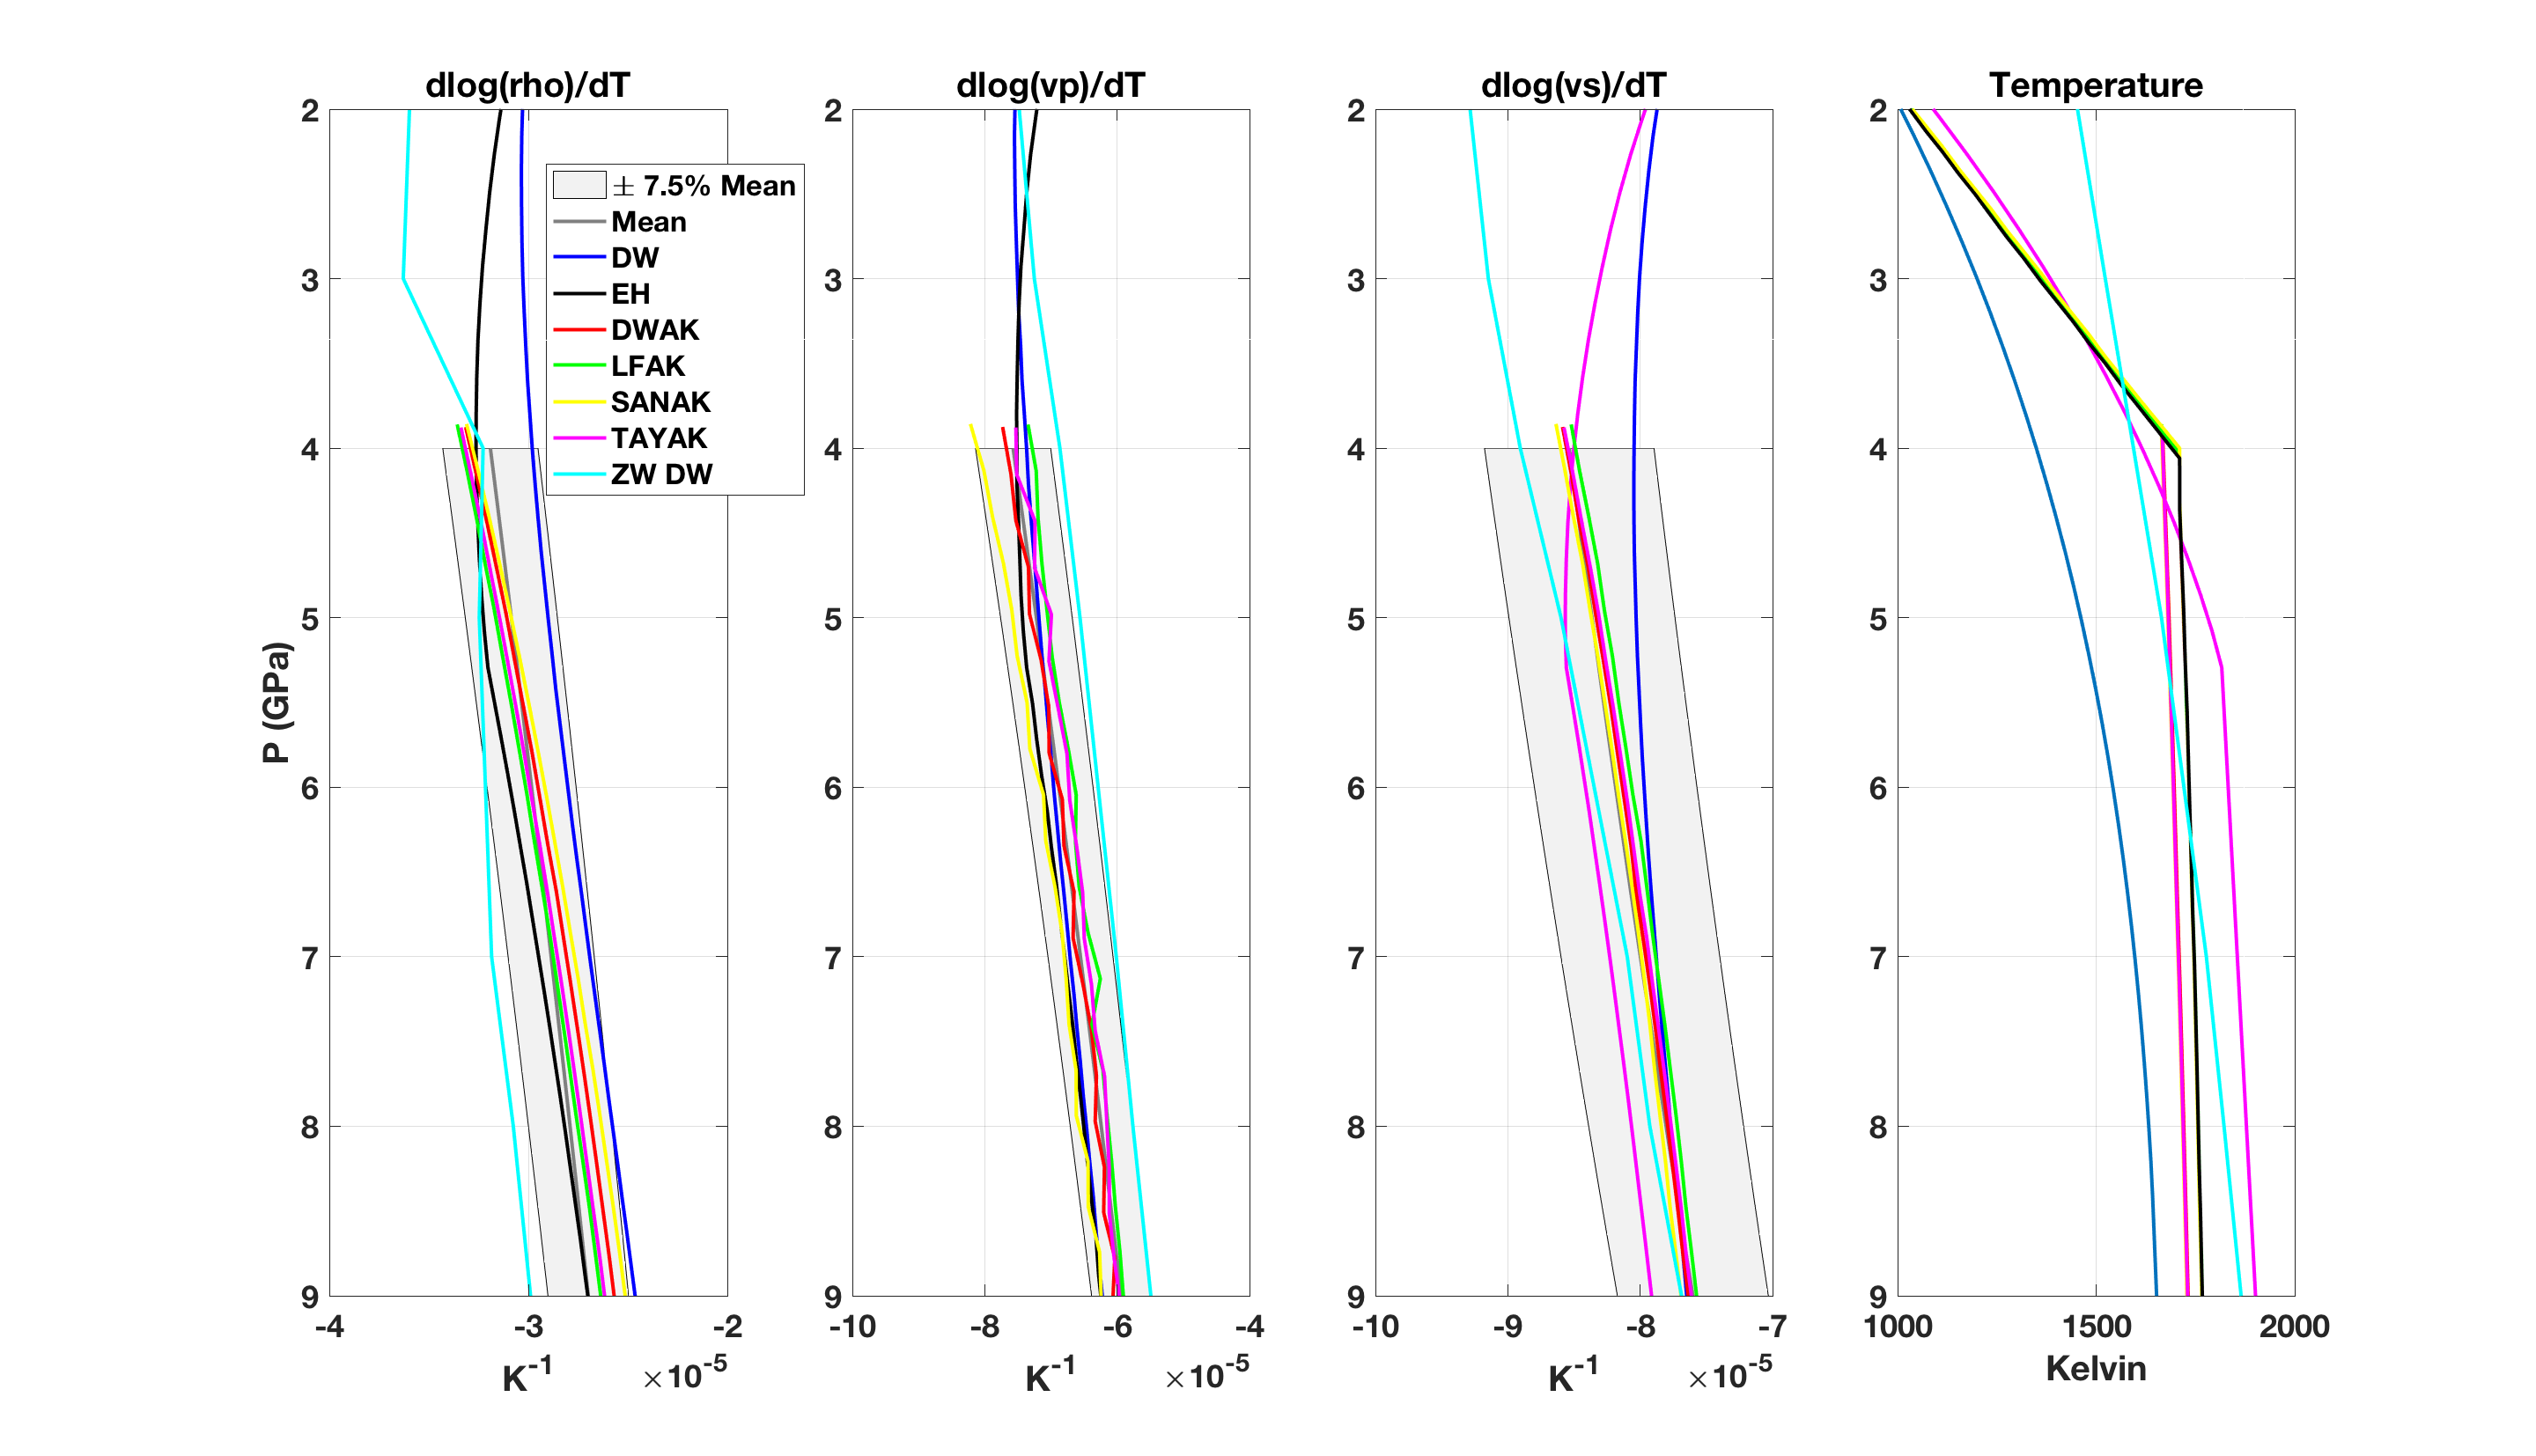
\includegraphics[width=1.0\textwidth]
{figures/Fig20_Interior_updated}
\caption{Temperature dependence of the reference models density and seismic velocities, together with mantle temperature of these models up to 8 MPa (about 600 km depth). These temperature dependencies are computed with a fixed mineralogy, which may be the case in the martian lithosphere. From left to right, the relative density, vp and vs sensitivities and the mantle temperature, at constant pressure. Grey zone is the $\pm$ 7.5\% area with respect to the mean sensitivity models, as defined in text and in Table ~\ref{table:TableEmp}.}
\label{fig:Fig20_Interior.png} 
\end{center}
\end{figure}

\begin{figure}[h!]
\begin{center}
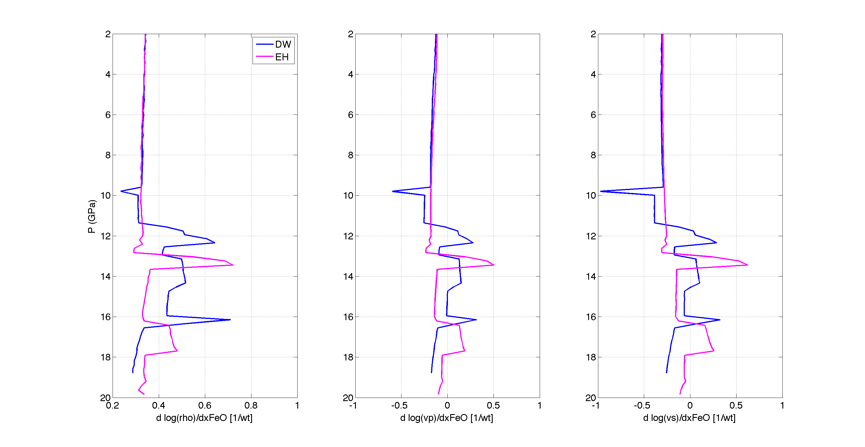
\includegraphics[width=1.0\textwidth]
{figures/Fig3-3-3.png}
\caption{Dependence of DW and EH45 models to FeO content.}
\label{fig:Fig3-3-3.png} 
\end{center}
\end{figure}

As shown in Section 3.1, large temperature variation are expected in the Martian lithosphere, mostly due to the large crustal heating lateral variations and to the large elastic lithosphere thickness, which allows such temperature lateral variation to be maintained over geological times. At 200 km depth, these temperature variations can be $\pm$150$^{\circ}$C for the models with the smallest variations, but can be up to $\pm$535$^{\circ}$C for those with the largest.
As seen above, the temperature sensitivities of both seismic velocities and densities are not strongly dependent on the type of models. We show furthermore that a simple linearized model can therefore parameterize these temperature variations. Figure~\ref{fig:Fig3-3-4.png} shows, for model TAY, the case of the largest temperature differences, i.e. 500$^{\circ}$C at the base of lithosphere for the and compare the non-linear $V_S$ computation $V_S$(T+DT) with the linearized one, $V_S$(T)+$\Delta$T $\times$ d$V_S$/dT. This error is about 10\% of the relative velocity change in the upper mantle, which is less than 0.4\% of the absolute Vs velocity. This error is also 10 times less than the L2 InSight/SEIS mission requirement for the determination of the mantle velocity ($\pm$0.25km/s and therefore about $\pm$6\%) and will therefore be much less than the capability of the mantle structure determination with a single station.

\begin{figure}[h!]
\begin{center}
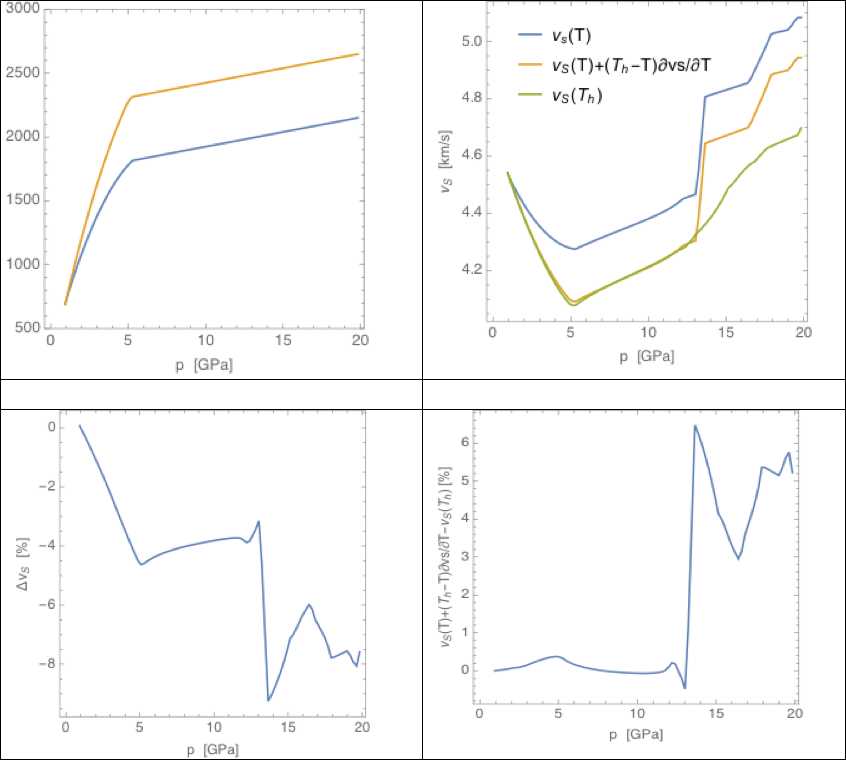
\includegraphics[width=0.8\textwidth]
{figures/Fig3-3-4_v2.png}
\caption{Temperature linearization error. From top left to top right. The two temperature model used and the obtained seismic velocity models, compared with the linearized model. Bottom left to bottom right: relative Vs variation between the two models and the error between the non-linear and linear case, in \%.}
\label{fig:Fig3-3-4.png} 
\end{center}
\end{figure}

\subsubsection{Vp,Vs, density 3D lateral variation}

In the following, we review the present-day possible density and body waves velocity anomalies due to lateral thermal and compositional heterogenetities present within Mars' silicate envelopes. In performing this exercise, one should stress that the presence of that lateral anomalies, even of significant amplitude, does not necessarily imply their unambiguous detection and characterization. This aspect will also be discussed in this section.  

\paragraph{Crustal Heterogenities}

Mars silicate envelope exhibits a variety of ranges for lateral variations in density ($\rho$) and body wave speeds ($v_p$, $v_s$) along its planetary radius, $r$. While the shallow crustal region appears to be characterized by the largest lateral variations, deeper regions are nonetheless also associated with important variations in $\rho$, $v_p$, and $v_s$.

At the surface, the crust can be roughly divided into two/three main domains (e.g., \citep{Solomon1982,Zuber2000,McSween2003}):
\begin{itemize}
  \item The northern lowlands, having a uniformly thin crust ($\sim$30 km on average) mostly composed of andesitic rocks and/or altered basalts.
  \item The southern highlands, consisting of a thick crust ($\sim$60 km on average) mostly composed of basaltic rocks. 
  \item The Tharsis Rise, located at the boundary between these two domains, where intense plume activity formed a thick ($\sim$100 km) basaltic crust.
\end{itemize}


At depth, one can expect these domains to be subdivided into different units, characterized by the following ranges, whose values are mostly inspired by \citet{Mavko2009}: 
\begin{itemize}
	\item Between 0 and 5 km depth, a heterogeneous superficial crust where various types of rocks coexist (sedimentary and igneous), leading to a wide range of densities and seismic velocities, from altered basalts ($\rho$=2700-3100 kg/m$^3$; $v_p$=5-6 km/s; $v_s$=2.8-3.4 km/s) to mudstones, shales, clays, sands and loess ($\rho$=1500-2500 kg/m$^3$; $v_p$=0.5-3.5 km/s; $v_s$=0.2-1.7 km/s). Moreover, different types of anisotropy could further affect the seismic velocities, such as sedimentary or lava flow layering (12-15\% variation), and the presence of wide damage zones surrounding long-term fault networks. Indeed, many studies have shown that damage zones could reduce seismic velocities from 10\% to 50\% depending on the structural maturity of the fault and regardless the geological context (see a compilation on Earth in \citet{Perrin2016}, their table S5). \citet{Cochran2009} also documented seismic velocities reduced by 40-50\% across a fault zone of 1.5 km wide in the Mojave Desert, which can be considered as a good geological analog for Mars (e.g., \citep{Golombek1997,Marlow2008}).
    \item The lithostatic pressure increase could result in a 10-12\% increase in velocities for sandstones between 0 and 50 MPa due to porosity reduction \citep{Han1986}.
    \item Between 5 and 15-20 km depth, an upper crust mostly formed by more differentiated volcanic materials, such as andesite, or altered basaltic rocks ($\rho$=2400-2800 kg/m$^3$; $v_p$=4.5-6 km/s; $v_s$=2.5-3.3 km/s). The variation of seismic velocity can still be affected by the layering of lava flows. However, below 5 km depth, fault damage zones become considerably reduced (e.g., \citep{Ben-Zion2003,Finzi2009,Allam2014} for studies on Earth), therefore limiting the lateral effect on seismic velocities. The gravity being smaller on Mars than on Earth, this depth may be larger than the aforementioned value.
    \item Between 15-20 and 30-100 km depth, a lower crust mainly composed of compacted basalts ($\rho$=2700-3100 kg/m$^3$; $v_p$=5-7.2 km/s; $v_s$=2.8-4 km/s), where various types of seismic anisotropy (lithological, structural, or stress-induced) can possibly occur (yielding an anisotropy up to 15-30\% on Earth, e.g., \citep{Crampin1991,Weiss1999}.
\end{itemize}


Figure~\ref{fig:lateral_lithosphere_anomalies}a-c summarizes the aforementioned plausible ranges of lateral crustal variations in density and body wave speeds.
Note that Mars' deep crustal density range has recently been questioned on the basis of in-situ chemical composition analyses, GRS maps, and SNC meteorites analysis \citep{Baratoux2014}. This has led to a higher range for crustal densities ($\sim$ 3100-3600kg/m$^3$), which may imply a deeper extent of Mars' crust in order to satisfy constraints on the moment of inertia. Although a deep eclogitic root would be gravitationally unstable and more easily prone to delamination, the larger crustal viscosities at such colder depths may efficiently delay in parts delamination processes, depending on the activation energy of the crustal material. For now, we will restrict our expectations to the more conservative estimates displayed in  Figure~\ref{fig:lateral_lithosphere_anomalies}a, however InSight's expected seismic record and heat flux measurements would allow the possibility of a deep ($\sim$ 100-200 km thick) eclogitic root to be tested.

\begin{figure}[h!]
\begin{center}
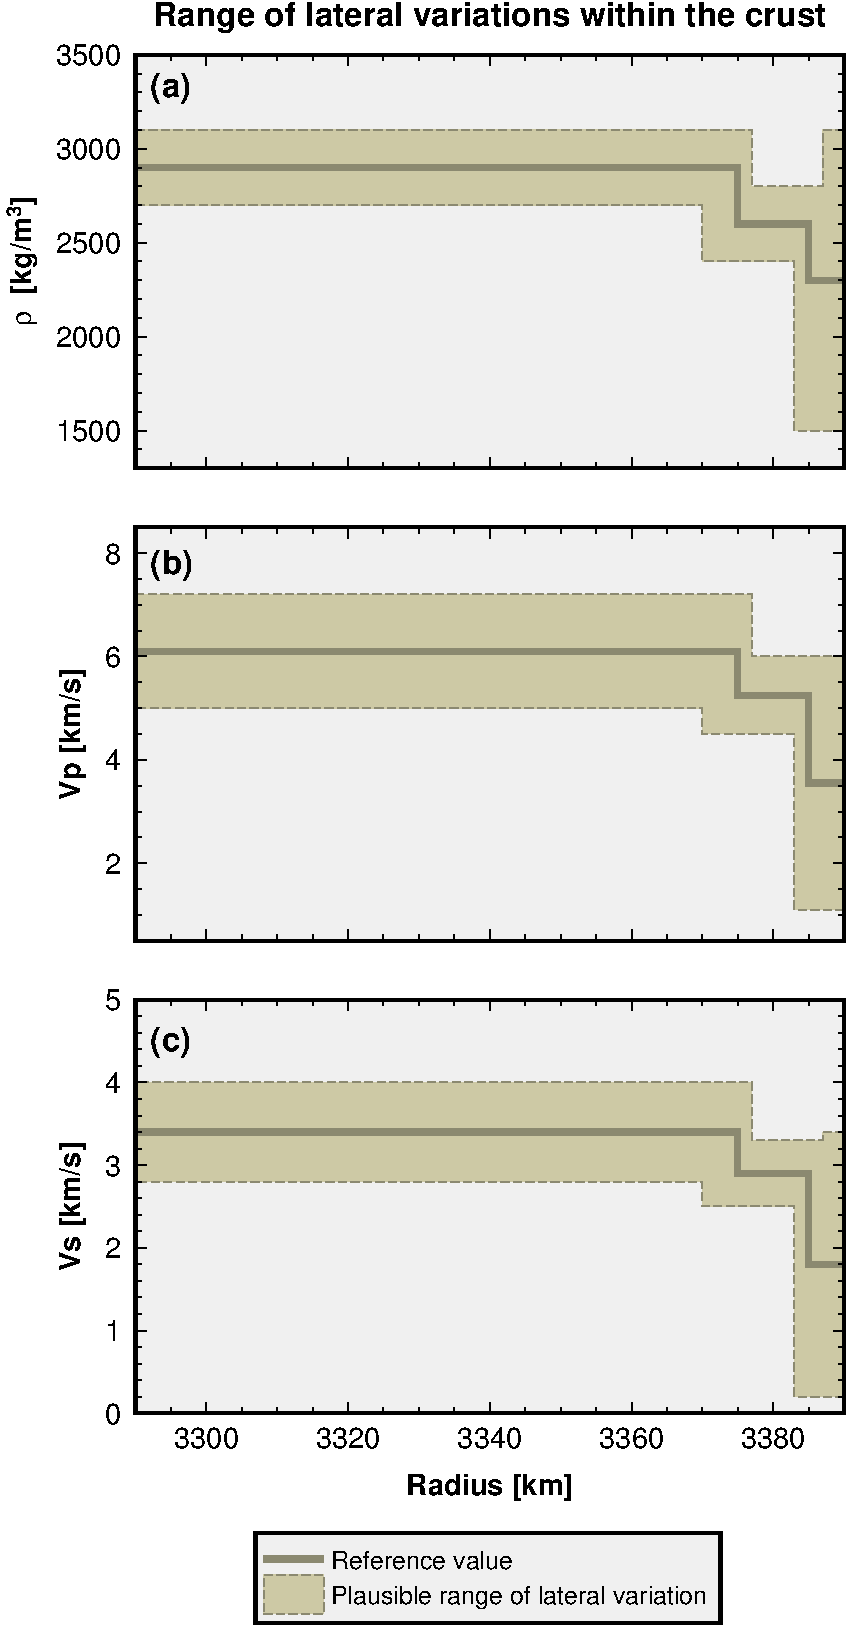
\includegraphics[scale=0.5]
{figures/Lateral_het_crust.pdf}
\caption{Plausible range of lateral crustal variations in density (a), P-wave (b) and S-wave (c) velocities within Martian crust region. See text for further details.}
\label{fig:lateral_lithosphere_anomalies}  
\end{center}
\end{figure}

In addition to lithological/petrological differences, the highlands and the lowlands are also expected 
to exhibit a distinct temperature structure. The southern hemisphere could be more than 300K hotter than the northern hemisphere over depths greater than 250 km, as a result of their different thicknesses and heat-producing element contents, as further discussed below.


\paragraph{Lithosphere and Mantle Heterogeneities}
In the deeper lithospheric region, changes in composition and (P,T) conditions lead to different ranges of lateral variations. The likely convective style of present-day Mars mantle corresponds to a stagnant-lid regime, in which a thick cold and highly viscous lithosphere (i.e., the lid) overlays a convective mantle. Lateral heterogeneities in the lithospheric region may result from variations in the thickness of the crust and the stagnant lid. The latter are mainly controlled by the interplay between rheology, heterogeneous internal heating due to variable enrichment in heat producing elements, and convective processes (e.g., \citep{Plesa2016} and references therein; \citep{Thiriet2018}). These constraints can be incorporated into numerical models of solid-state convection with temperature-dependent viscosity, conducted in spherical geometry. In this context, we have considered two end-member cases. 
One reference model discussed in section~\ref{ref_temp}, having a strong pressure-dependence of viscosity, with an activation volume of 10 cm$^3$/mol, and matching a number of observational constraints (past and present elastic thicknesses, volcanism etc., see section 3.1). 
We also considered a second case, which only differs from the reference model by the fact that  viscosity does not depend on pressure. This model produces small temperature variations in the convecting mantle, comparable to the cold end-member case considered in section ~\ref{ref_temp} and Table~\ref{table:end_member_ref_models}.
Lateral anomalies in density and body-waves speeds can then be estimated along the planetary radius using conversion coefficients $\partial \ln\rho/\partial T$, $\partial \ln v_p/\partial T$, $\partial \ln  v_s/\partial T$ derived from Gibbs free-energy minimization, and the latter are described in section 3.2. Variations in crustal and lithosphere thickness yield important peak-to-peak temperature anomalies. Their plausible range are shown in Figure~\ref{fig:Fig4.png} and summarized in Table~\ref{table:T_induced_variations} for two extreme temperature models (high and  low $\delta T$) and for the reference model described in section~\ref{ref_temp} (Table~\ref{table:end_member_ref_models}). 

\begin{table}[h!]
\centering
\caption{Plausible ranges of lateral variations in temperature, and temperature-induced density and seismic velocity variations. Sensitivities range are set to -2.5/-3.5 10$^{-4}$ K$^{-1}$, -6.5/-7.5 10$^{-4}$ K$^{-1}$, -8/-9 10$^{-4}$ K$^{-1}$ for density, $v_p$ and $v_s$ respectively. The three temperature models are those of section~\ref{ref_temp} .}
\begin{tabular}{l|lllll}
                            & Min. T& Max. T & $\delta\rho/\rho$   & $\delta v_p$/$v_p$ & $\delta v_s$/$v_s$        \\ \hline
Low $\delta T$ Model        & 1016  & 1316   & 0.8/1.1\%      & 2/2.3\%       & 2.4/2.7\% \\
Reference $\delta T$ Model  & 791   & 1795   & 2.5/3.5\%      & 6.5/7.5\%     & 8/9\%     \\
High $\delta T$ Model       & 629   & 1700   & 2.7/3.7\%      & 7/8\%         & 8.6/9.6\%
\end{tabular}
\label{table:T_induced_variations}

\end{table}

Such variations in crustal and lithospheric thicknesses yield important peak-to-peak anomalies $\delta \rho$=2-3.5\%, $\delta  v_p$=6-8\%, $\delta  v_s$=8-10\% for the reference and high $\delta$T models.  These are also imaged in Figures~\ref{fig:lateral_mantle_anomalies}a-c, which show that lateral variations in density and body wave speeds are more pronounced for the case with pressure-dependent viscosity, as it generates larger temperature variations that erode the cold lid more efficiently.

\begin{figure}[hp!]
\begin{center}
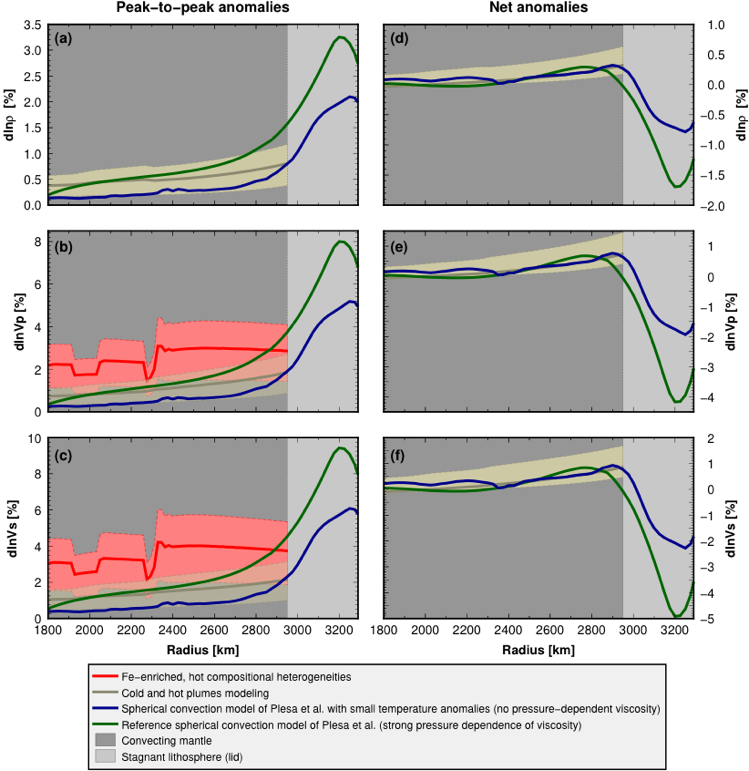
\includegraphics[width=1.0\textwidth]
{figures/Fig3-3-3-3.png}
\caption{ Left (a-c): peak-to-peak lateral anomaly profiles for density (top), P-wave speed (middle), and S-wave speed (bottom) as a function of Mars radius, $r$. The beige colored area corresponds to the contribution of cold and hot axisymmetric plume conduits, obtained from numerical modeling. This area is bounded by two extreme cases (dashed brown curves). The lower bound corresponds to the following governing parameters: $Ra=10^5$, $E$=540 kJ/mol, and temperature contrast across the lower thermal boundary layer $\delta_{\rm TBL}$=50 K. The upper bound corresponds to $Ra=10^7$, $E$=200 kJ/mol, $\delta_{\rm TBL}$=100 K. An intermediate case is shown (thick brown curve) for $Ra=10^6$, $E$=300 kJ/mol, $\delta_{\rm TBL}$=100 K. The anomalies derived from the thermal structure of two spherical thermal convection models are also shown: a case with no pressure dependence of viscosity (blue curves), and yielding the smallest temperature anomalies, and a case with strong pressure-dependent viscosity (green curves). The latter model, described in section 3.1, explains best observational constraints. Anomalies associated with the presence of purely hotter and denser (Fe-enriched) compositional heterogeneities for a range of compositional density contrasts 0.5-1.5\% (light red area bounded by dashed red curves for $\delta \rho_c$/$\rho$=0.5\% and $\delta \rho_c$/$\rho$=1.5\%). The case for $\delta \rho_c$/$\rho$=1\% is illustrated with the thick red curve. Right (d-f): net anomalies resulting from summing the anomalies associated with cold and hot material, which are of opposite sign. These correspond to the same models considered in (a-c), with the exception of the anomalies associated with compositional heterogeneities. See text for further details.}
\label{fig:lateral_mantle_anomalies} 
\end{center}
\end{figure}

The largest shallow temperature variations are however expected to be localized beneath Tharsis and Hellas, and will be detected only for rays passing through. Figure~\ref{fig:Fig3-3-3-2.png} provides, for the three proposed temperature models shown in Table~\ref{table:end_member_ref_models}, the cumulative curve of area percentage at a given temperature at 200km depth.  For the reference model, temperature varies by somewhat less than 300K across 80\% of the surface for the nominal case, reducing the  $v_s$ seismic velocity lateral variations to less than 3\% peak-to-peak, which is  about half the L2 InSight/SEIS mission requirement for the determination of the mantle velocity ($\pm$0.25km/s, therefore, about $\pm$6\%).

\begin{figure}[h!]
\begin{center}
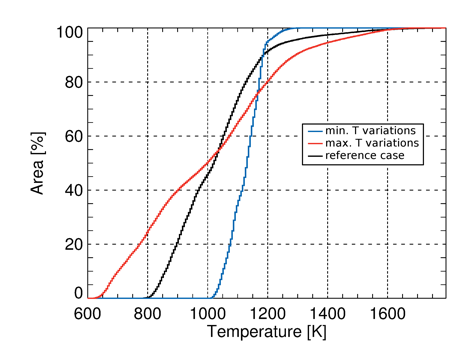
\includegraphics[scale=0.95]
{figures/Fig3-3-3-2.png}
\caption{Cumulative histogram showing the fraction of the surface of Mars at 200km depth where the temperature lies below a given value. The three lines correspond to the three models described in section~\ref{ref_temp}.}
\label{fig:Fig3-3-3-2.png} 
\end{center}
\end{figure}

At greater depths, lateral heterogeneities in present-day Mars mantle most likely result from solid-state convective processes. In the simplest case of purely thermal convection, temperature anomalies, $\delta T$, result from hot upwelling and cold downwelling plume conduits originating from core-mantle, and surface thermal boundary layers (TBL), respectively. To first-order, plumes are axially symmetric objects whose radius $R_p$ broadens with the plume height, $h_p$, as a result of thermal diffusion. The temperature anomaly is maximum along the plume centerline, and decreases away from it. Plume broadening also results in a progressive decrease of the amplitude of thermal anomalies between the plume and its surroundings. These characteristics were predicted by theory \citep{Batchelor1954,Whittaker2006} and were confirmed by laboratory and numerical experiments (\citep{Davaille2011,VanKeken2013}, and references therein). These studies have shown that $R_p \sim (h_p-h')^{1/2} Ra^{-\beta}$, and that the plume centerline temperature $T_c \sim 1/(h^*+h_p) \sim \delta T$, where $Ra$ is the effective Rayleigh number expressing the convective vigor of the mantle, and $\beta \cong $0.2 \citep{Lithgow-Bertelloni2001} . The functions $h^*$ and $h'$ depend on $Ra$, and on the viscosity contrast across active (i.e., mobile) parts of the TBLs, $\Delta \eta$. The latter differ in cold and hot TBLs due to the temperature dependence of viscosity through an activation energy, $E$ (e.g., \citep{Karato1993}), and due to the different amplitudes of temperature variations, $\delta_{\rm TBL}$, across the cold and hot TBL, implying that cold and hot Martian plumes have likely different strengths. The above relationships indicate that the main governing parameters for the temperature anomalies associated with plumes are $Ra$ and $E$, $\delta_{\rm TBL}$ (or equivalently $\Delta \eta$), whom values remain poorly constrained. We computed temperature anomalies associated with cold and hot plumes using high-resolution finite-volume discretization of the Navier-Stokes and the conservation of internal energy equations in axi-symmetric geometry, with temperature-dependent viscosity, under the infinite Prandtl number and Boussinesq approximations \citep{Samuel2012}. 

With the knowledge of plume thermal structure, lateral anomalies in density, $v_p$, and $v_s$ can be estimated along the planetary radius using conversion coefficients, as previously explained. The obtained values for $v_p$ and $v_s$ anomalies are averaged over spherical regions with a radius of 15 km and 10 km corresponding to typical sizes of Fresnel zones for P and S waves, respectively.

It should be noted that phase transitions occurring within Mars' mantle (e.g., olivine-wadsleyite and wadsleyite-ringwoodite) could produce peak values in relevant derivatives of thermoelastic properties \citep{Stixrude2007}. The details  depend on the details of the specifics of the compositional models Figure~\ref{fig:Fig_dT.png} and the iron content Figure~\ref{fig:Fig_dFeO.png}. These would result in possibly large amplitude peaks in $d\ln \rho$, $d\ln v_p$, $d\ln v_s$. However, the amplitude of such peaks depends on poorly constrained values of physical parameters such as the Clapeyron slope and the pressure range over which the phase transitions occur. In addition, these peaks are likely to be very narrow. For these reasons, the conversion coefficients $\partial \ln\rho/\partial T$, $\partial \ln v_p/\partial T$, and $\partial \ln v_s/\partial T$ we used to infer the anomalies displayed in Figure~\ref{fig:lateral_mantle_anomalies} correspond to isomorphic contributions. 



Figure~\ref{fig:lateral_mantle_anomalies}a-c shows the plausible range of peak-to-peak (i.e., from hot to cold plumes) lateral anomaly profiles along $r$ (inferred from the plausible ranges for $Ra=10^5-10^7$, $\delta_{\rm TBL}$=50-100 K for the bottom TBL, $\delta_{\rm TBL}$=100-200 K for the (mobile) part of the upper TBL, and $E$=200-540 kJ/mol). Upper and lower TBLs were not included since purely lateral thermal anomalies would vanish in these regions. The median values range between 0.5\% and 1\% $\pm$ 1\%. $v_s$ anomalies are more pronounced than $v_p$, due to the higher sensitivity to temperature of the shear modulus compared to that of the bulk modulus. The increase of lateral anomalies with increasing $r$ primarily results from the pressure-dependence of physical properties (bulk and shear moduli, $\rho$, and their temperature dependence), and secondarily from the asymmetry between stronger cold and weaker hot plumes at a given $Ra$ value, leading to an increase in peak-to-peak temperature anomalies with increasing $r$. 

This simple plume modeling approach does not account for additional potential complexities of Martian mantle dynamics such as plume interactions, pressure-dependent viscosity \citep{Leng&zhong2008}, the presence of a heterogeneous crust of variable thickness, phase changes, or sphericity. Such complexities may in particular enhance the top-bottom asymmetry between upwellings and downwellings or could affect the thermal structure of plume conduits. To assess such influences we have considered the thermal structure derived from the two models in spherical geometry mentioned above (the blue and green curves in Figure~\ref{fig:lateral_mantle_anomalies}). The model with no pressure dependence of viscosity (blue curves in Figure~\ref{fig:lateral_mantle_anomalies}a-c) agrees well with the lowest end of lateral anomalies inferred from the plume modeling. The second model with strong pressure-dependence of the viscosity exhibits peak-to-peak anomalies in the lowermost mantle that are smaller than the plausible range covered by the plume model (green curves in Figure~\ref{fig:lateral_mantle_anomalies}a-c). However, the more pronounced top-bottom asymmetry (enhanced by pressure-dependent viscosity) leads to an increase in anomalies with $r$, to values larger than the plume models at shallower depths. 

The possibility of thermo-chemical convection suggested by the identification of geochemical reservoirs within Mars mantle through the analysis of the SNC meteorites \citep{Debaille2007} should also be considered. In this case, the survival of compositional heterogeneities in a convective mantle most likely occurs through the presence of denser (possibly Fe-enriched) material, which gradually heats up, as it does not participate in convection \citep{Samuel2003}. Such a hot and denser material must remain sufficiently stable to prevent convective mixing, and sufficiently buoyant to be sampled and brought to the surface by upwelling plumes, as suggested by the analysis of the SNC meteorites. This can occur provided that the compositional density contrasts and thermal density contrasts remain comparable: $\delta \rho_c/\rho \sim \alpha(r)\delta T(r)$ \citep{LeBars2004}. This constraint yields a rough estimate for $\delta T(r)$, assuming that the other parameters are reasonably well known. We used $\alpha(r)$ from DW, see section 3.4.2. Numerical experiments \citep{Tosi2013} have suggested that a plausible range for  $\delta \rho_c/\rho$ would be about 0.5\%-1.5\%. Such a range is considered in Figure~\ref{fig:lateral_mantle_anomalies}a-c, and yields the largest peak-to-peak anomalies in the convective mantle, despite the fact that cold plume contributions were not even considered for this case. Note that $v_p$ and $v_s$ anomalies also account for the Fe-enrichment assumed for the denser material, but this influence is minor compared to the temperature effect. Although their size, shape and volume are largely unconstrained, such hypothetical compositional heterogeneities could significantly contribute to lateral heterogeneities within the deep Martian mantle.

Finally, as pointed out earlier, the presence of lateral anomalies within Mars' mantle can be clouded in a number of ways. 
A good example of the difficulty in detecting and characterizing lateral seismic anomalies is the Earth's mantle, where density and seismic velocity anomalies of comparable or larger amplitudes than those discussed in this section remain difficult to image. Indeed, despite an obviously much denser seismic array, and vast amounts of high-quality data, the seismic detection of mantle plume anomalies on Earth remains debated (\citep{Montelli2004,VanderHilst2006} and references therein), and in the best case is prone to trade-offs between the size of the anomalies and their amplitude \citep{French2014}. 
The difficulty in detecting lateral anomalies could result from a number of processes, such as the sampling of anomalies of smaller size than the wavelength of the seismic waves, the presence of sharp velocity gradients along interfaces with a possibly complex topology triggering multiple reflections, the development of shadow  zones associated with slow velocity anomalies, etc.

In addition, the opposite signs of $\partial \ln\rho / \partial T$, $\partial \ln v_p / \partial T$, $\partial \ln v_s/ \partial T$ associated with cold and hot anomalies may, to some extent, cancel out each other, as seismic waves integrate positive and negative anomalies along their paths. This last possibility is illustrated in Figure~\ref{fig:lateral_mantle_anomalies}d-f where the resulting net sum of hot and cold anomalies shown are two to four times smaller than peak-to-peak anomalies (Figure~\ref{fig:lateral_mantle_anomalies}a-c). While this outcome depends on a number of unknown parameters such as the distribution of hot and cold anomalies, or source locations, it underlines the fact that canceling lateral anomalies may hinder the presence of heterogeneities of much larger amplitude.
More generally, it is likely that the SEIS experiment would only detect a smaller fraction of the anomalies predicted in Figures~\ref{fig:lateral_lithosphere_anomalies} and Figures~\ref{fig:lateral_mantle_anomalies}a-c.
However, the expected important temperature differences over a significant lithospheric depth range between the southern and the northern hemisphere would be sufficiently large to allow for a seismic detection by surface waves, provided a favorable location of the seismic sources \citep{Panning2016}.
The seismic detection of the north-south dichotomy (or even its non-detection) by SEIS would provide important information regarding the present-day thermal state or Mars, and/or the rheological properties of its silicate envelope. Additionally, the IFG will provide magnetic field measurements at the Martian surface. If separable from fluctuations due to the lander, periodic variations in the Martian magnetic field will be monitored and recorded. Such variations have already been observed in orbit (Langlais et al., 2017; Mittelholz et al., 2017). The analysis of these measurements may provide more robust constraints on the electrical conductivity profile at depth, which, when combined with velocity profiles derived from SEIS, should improve models of the interior of Mars.


\begin{figure}[h!]
\begin{center}
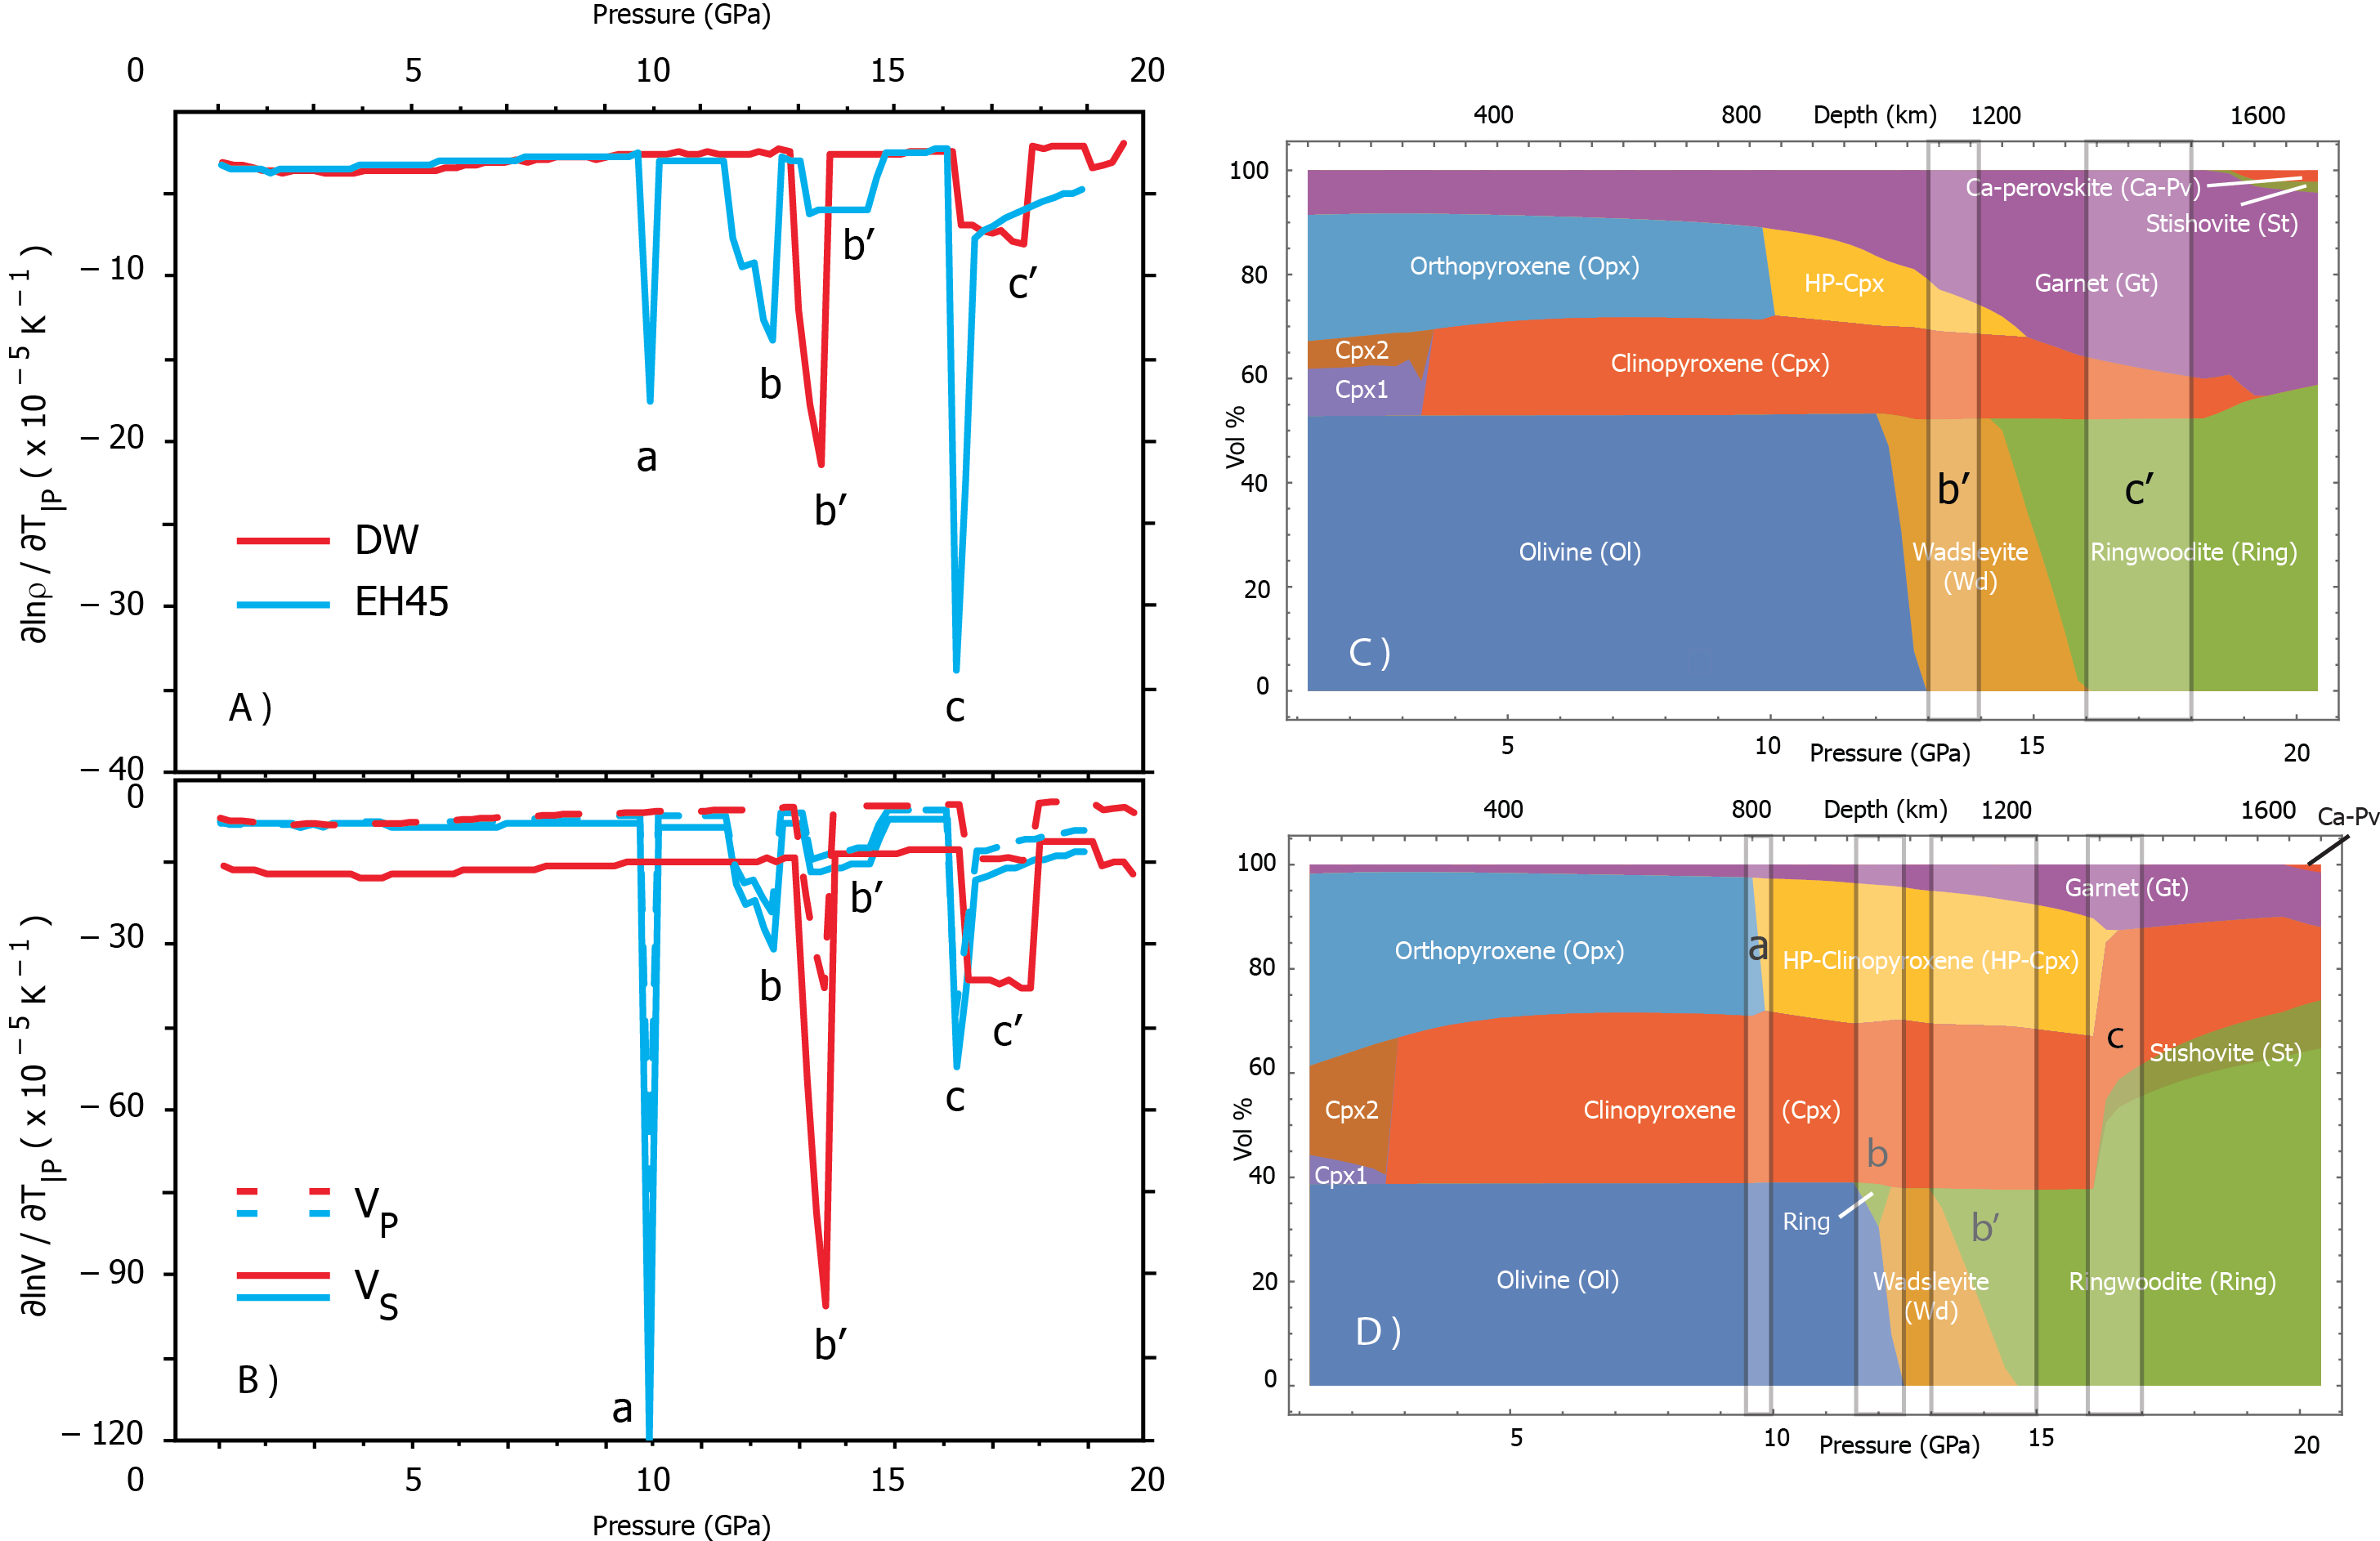
\includegraphics[width=1.0\textwidth]
{figures/Fig_dT.png}
\caption{Two examples of the temperature dependence of Mars' mantle models. DW : olivine-rich composition of \citet{Dreibus1984} revised in \citep{Taylor2013}; EH45 : pyroxene-rich composition of \citet{Sanloup1999}. In the left panels the sensitivity of the density (A) and seismic velocities (B) to temperature perturbations are plotted as a function of pressure. The labeled peaks are induced by the mineralogical transformations displayed in the right panels for the DW (C), and EH45 (D) compositions.}
\label{fig:Fig_dT.png} 
\end{center}
\end{figure}

\newpage
\begin{figure}[!h]
\begin{center}
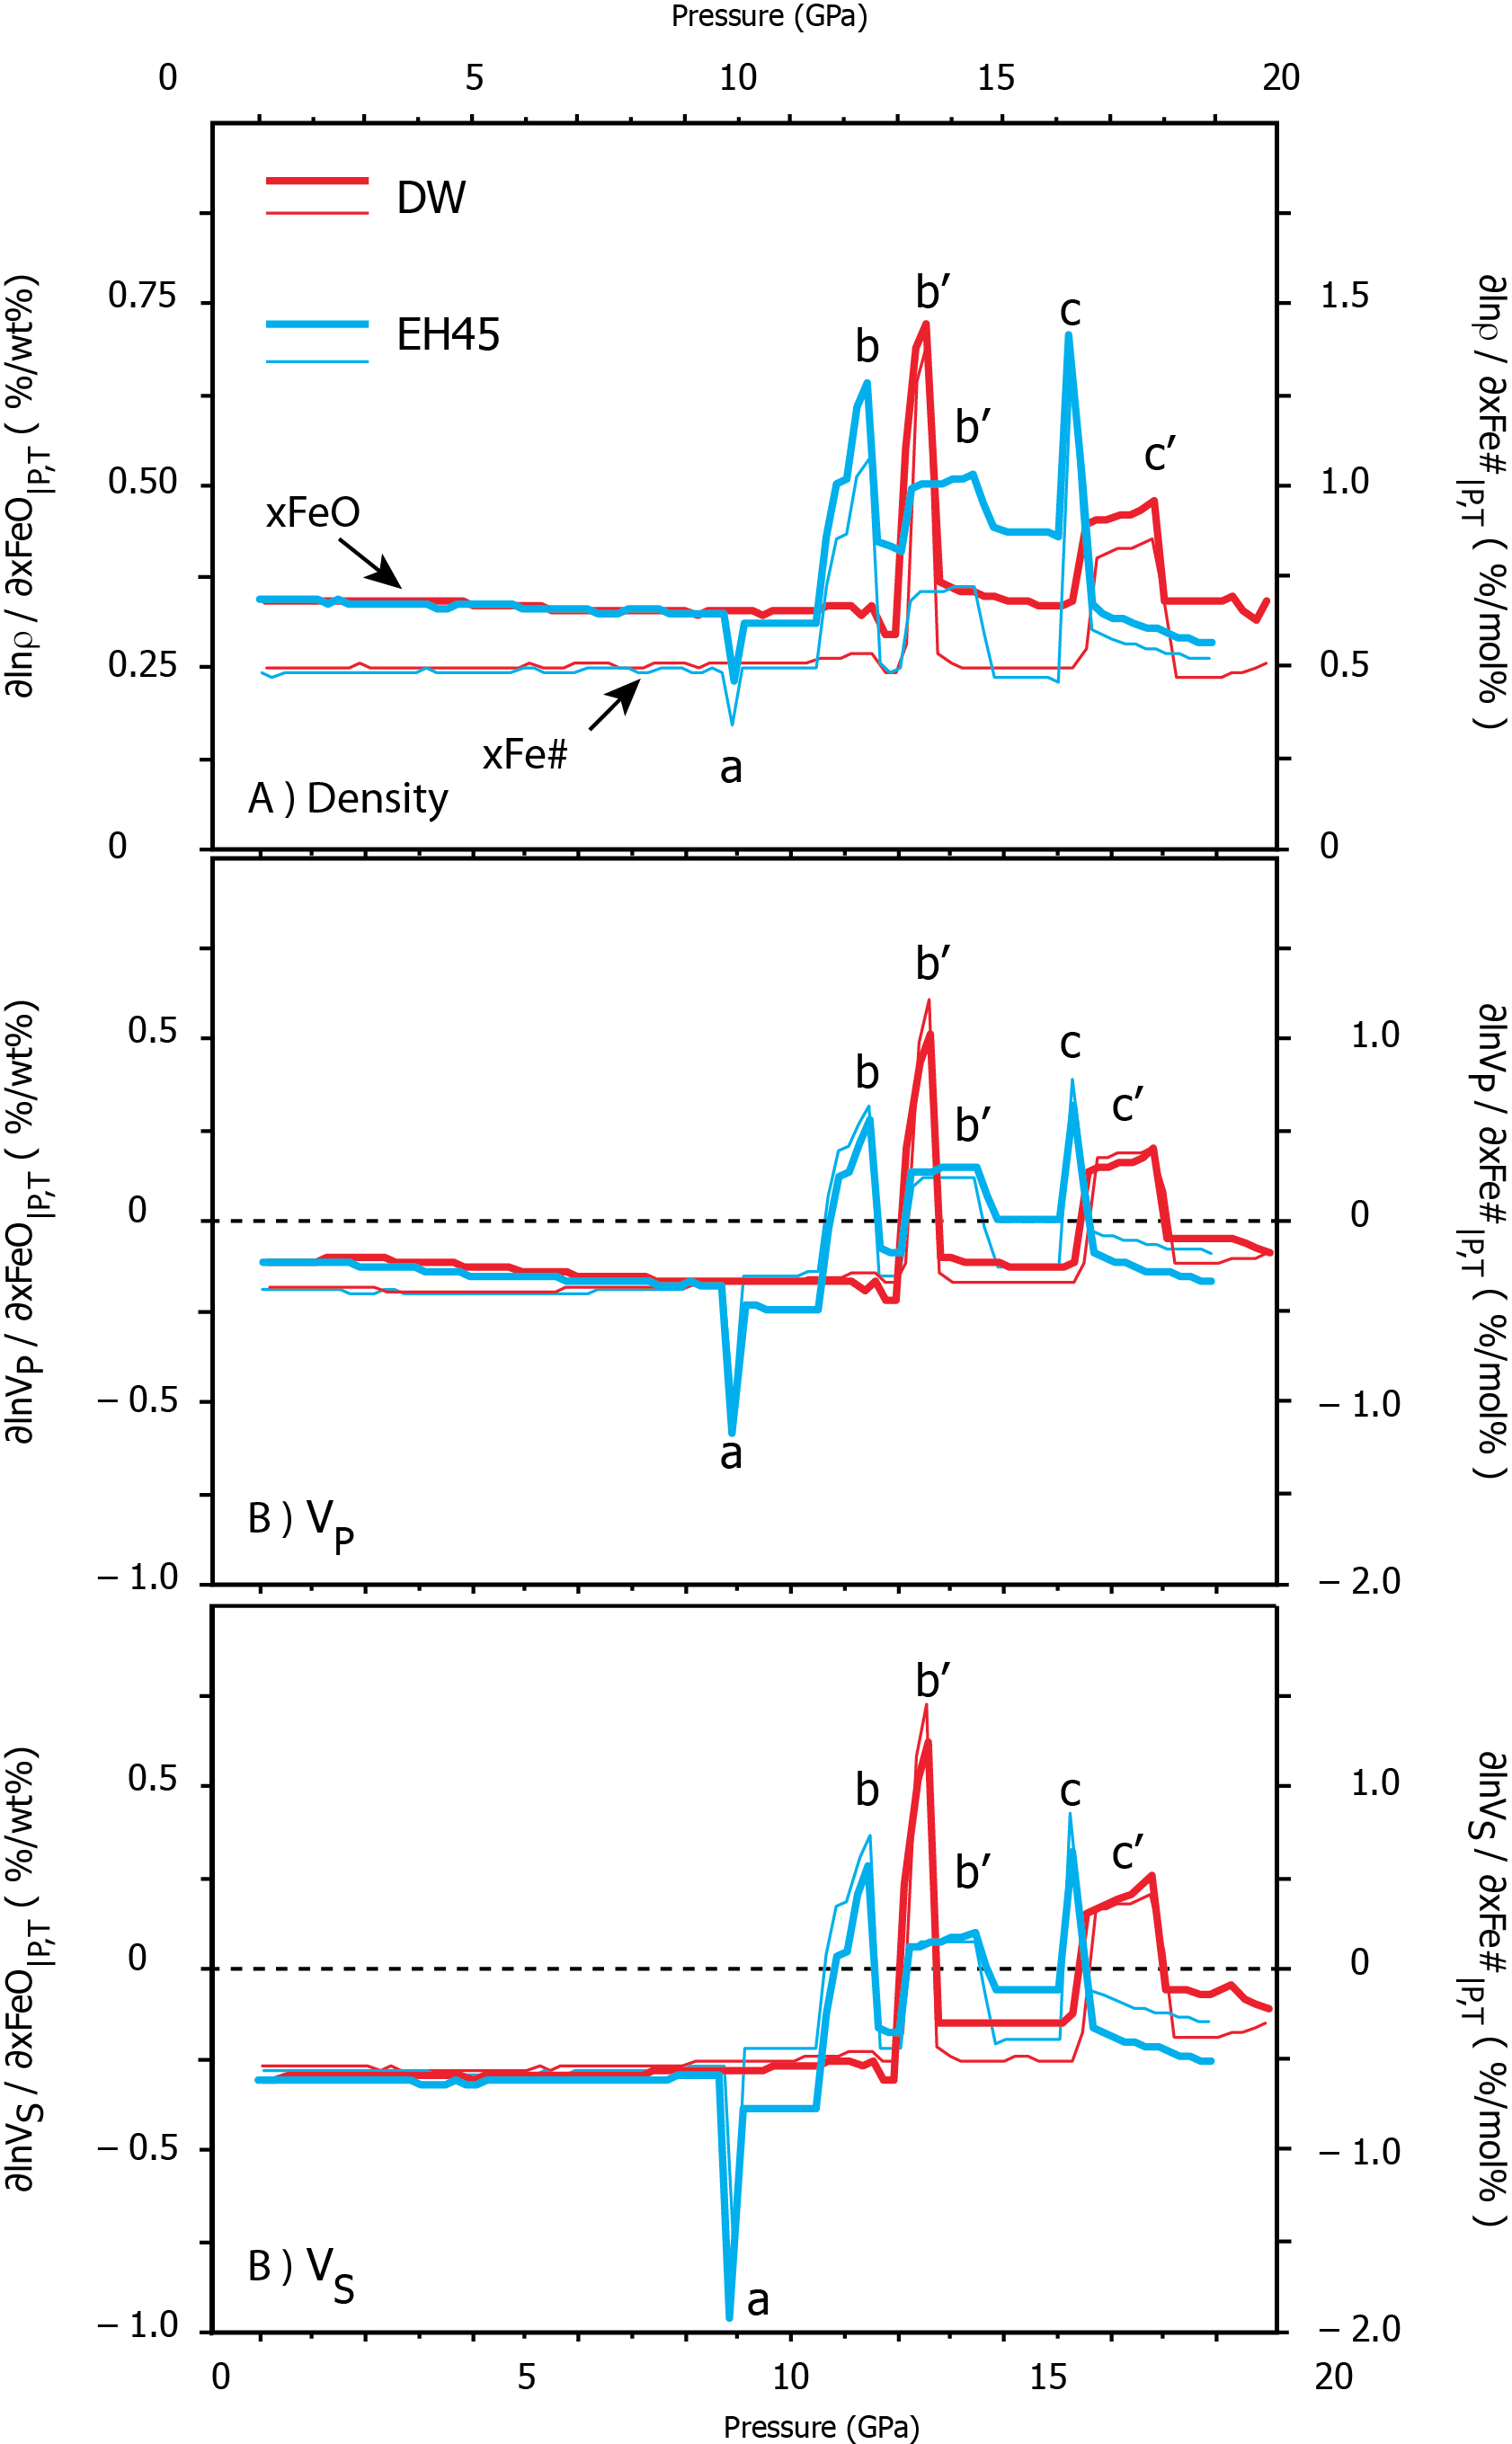
\includegraphics[width=1.0\textwidth]
{figures/Fig_dFeO.png}
\caption{Same as Figure~\ref{fig:Fig_dT.png} for the dependence on the FeO content. Heavy curves and left y-axis refer to a bulk variation of the FeO content. Thin curves and right y-axis refer to a molar Fe\# variation within the \ce{[Mg_xFe_{(1-x)}]O} compound. The labeled peaks refer to the mineralogical transformations illustrated in Figure~\ref{fig:Fig_dT.png}C and D.}
\label{fig:Fig_dFeO.png} 
\end{center}
\end{figure}

\newpage
\section{Summary\label{sec:summary}}This paper summarizes the state of knowledge of the interior structure and composition of Mars.  Our understanding of Mars’ evolution is highly dependent on estimates of key parameters.  InSight will determine Mars’ interior layering, core state, heat flux, and level of tectonic activity and meteorite impact rates Table~\ref{tab:uncertainty}. Uncertainty requirements are specified to levels necessary to both enable comparative planetology studies and to vastly improve the input parameters for models of thermal and chemical evolution of the interior.  At present, many of these parameters are very loosely constrained via indirect measurements Table~\ref{tab:uncertainty}. InSight will vastly decrease uncertainties, in some cases to ranges approaching those estimated for Earth.  Since the InSight proposal was written in 2010, only the estimate of core size has substantially improved.  As discussed above, new data for the planetary gravity field and rover tracking data have provided better k2 constraints, decreasing the uncertainty in core radius to approximately ± 100 km.  Core density is still poorly constrained and will be significantly aided by InSight measurements of core size and state.

Each individual measurement is an important key to Mars’ past evolution and current state. Collectively these data will yield a tremendous leap forward for understanding the tightly coupled processes of planetary thermal and chemical evolution.  For example, both seismic measurements and heat flow constrain present day temperature.   The mantle temperature is function of the concentration of radiogenic elements, any phase transitions, and heat coming from the core.  Seismic velocity helps constrain mantle temperature and water content.  The heat flux measured at the surface is the sum of mantle and core heat flux, with the dominant contribution from radiogenic elements in the crust.  By measuring crustal thickness, it becomes possible to constrain the relative contributions of the crustal and mantle contributions.  Similarly, these parameters are all interconnected with respect to Mars’ bulk composition.

The availability of meteorites and datasets from dozens of missions make Mars the best studied rocky planet beyond our own.  The data from InSight are necessary to make a huge leap forward in understanding Martian history, from its earliest formation, to differentiation, to formation of its atmosphere.  Many fundamental questions remain for Mars, such as: Is the interior composition chondritic? What phase transitions exist in the mantle?  Is the core fully liquid? Does the crust have layers? Are layers preserved from a magma ocean? What kinds of geologically processes are active today?  At what depth should water be liquid today, if present?  

Knowledge of rocky planetary interior structure and evolution is primarily based upon the abundant datasets available for the Earth, and secondarily from much more limited data for the Moon.  Our understanding of magma ocean processes and planetary differentiation is dominated by these two bodies with very different sizes and geologic histories.   The InSight data set will provide a window into a rocky planet that is large enough to have enough heat production to have an extended geologic history, but arguably small enough such that heat loss from the interior does not appear to have driven plate tectonics.  Unlike the Moon, Mars has an atmosphere and hydrosphere (now a cryosphere) a result of its larger size and extended volcanic activity.  Unlike Earth, stable surface water on Mars was short-lived.  In these and many other regards, Mars is substantially different from Earth and the Moon.  Data from InSight will enable a better understanding of the continuum of rocky bodies.




\begin{table}[h!]
\centering
\caption{Current state of knowledge of the interior of Mars and expected levels of uncertainty at the end of the InSight mission.}
\begin{tabular}{|l|l|l|}
\hline
\multicolumn{1}{|c|}{\textbf{Quantity}} & \multicolumn{1}{c|}{\textbf{Current Uncertainty}} & \multicolumn{1}{c|}{\textbf{Science Requirement}} \\ \hline
Crust Thickness                & ±35 km (inferred)                        & ±10 km                                   \\ \hline
Crust Layering                 & No knowledge                             & 0.5 km/s contrasts                       \\ \hline
Mantle Seismic Velocity        & ±1 km/s (inferred)                       & ±0.25 km/s                               \\ \hline
Core Radius                    & ±450 km                                  & ±200 km                                  \\ \hline
Core Density                   & ±1000 kg/m3                              & ±450 kg/m3                               \\ \hline
Core State                     & Likely liquid                            & Positive det.                            \\ \hline
Heat Flux                      & ±25 mW/m2 (inferred)                     & ±5 mW/m2                                 \\ \hline
Level of Activity              & Factor of 10 (inferred)                  & Factor of 2                              \\ \hline
Location of Activity           & No knowledge                             & ±25\% of distance                        \\ \hline
Impact Rate                    & Factor of 6                              & Factor of 2                              \\ \hline
\end{tabular}
\label{tab:uncertainty}
\end{table}




\textbf{Acknowledgements}
 
A portion of the work was supported by the InSight Project at the Jet Propulsion Laboratory, California Institute of Technology, under a contract with the National Aeronautics and Space Administration

\bibliographystyle{aps-nameyear}
\bibliography{InSight_Refs}



%\section{Introduction}
%\label{intro}
%Your text comes here. Separate text sections with
%\section{Section title}
%\label{sec:1}
%Text with citations \cite{RefB} and \cite{RefJ}.
%\subsection{Subsection title}
%\label{sec:2}
%as required. Don't forget to give each section
%and subsection a unique label (see Sect.~\ref{sec:1}).
%\paragraph{Paragraph headings} Use paragraph headings as needed.
%\begin{equation}
%a^2+b^2=c^2
%\end{equation}
%
%% For one-column wide figures use
%\begin{figure}
%% Use the relevant command to insert your figure file.
%% For example, with the graphicx package use
%  \includegraphics{example.eps}
%% figure caption is below the figure
%\caption{Please write your figure caption here}
%\label{fig:1}       % Give a unique label
%\end{figure}
%%
%% For two-column wide figures use
%\begin{figure*}
%% Use the relevant command to insert your figure file.
%% For example, with the graphicx package use
%  \includegraphics[width=0.75\textwidth]{example.eps}
%% figure caption is below the figure
%\caption{Please write your figure caption here}
%\label{fig:2}       % Give a unique label
%\end{figure*}
%%
%% For tables use
%\begin{table}
%% table caption is above the table
%\caption{Please write your table caption here}
%\label{tab:1}       % Give a unique label
%% For LaTeX tables use
%\begin{tabular}{lll}
%\hline\noalign{\smallskip}
%first & second & third  \\
%\noalign{\smallskip}\hline\noalign{\smallskip}
%number & number & number \\
%number & number & number \\
%\noalign{\smallskip}\hline
%\end{tabular}
%\end{table}

%\begin{figure}\sidecaption
%\resizebox{0.3\hsize}{!}{\includegraphics*{figure.eps}}
%\caption{A figure}
%\end{figure}

%\begin{acknowledgements}
%If you'd like to thank anyone,place your comments here
%and remove the percent signs.
%\end{acknowledgements}






\end{document}


